    % Para utilizar este template siga o tutorial disponível em http://www.biblioteca.ufc.br/images/arquivos/instrucoes_modelos/tutorial_sharelatex.pdf

%%%%%%%%%%%%%%%%%%%%%%%%%%%%%%%%%%%%%%%%%%%%%%%%%%%%%%%
%% Você deve criar uma conta no ShareLatex. Depois,  %%
%% vá nas opções no canto esquerdo superior da tela  %%
%% e clique em "Copiar Projeto". Dê um novo nome pa- %%
%% ra o projeto.                                     %%
%%                                                   %%
%% Os principais desenvolvedores deste template são: %%
%%                                                   %%
%%            Ednardo Moreira Rodrigues              %%
%%     (Doutorando em Engenharia Elétrica - UFC)     %%
%%                      &                            %%
%%            Alan Batista de Oliveira               %%
%%     (Graduando em Engenharia Elétrica - UFC)      %%
%%                                                   %%
%% Revisão:                                          %%
%%                                                   %%
%% - Eliene Maria Vieira de Moura;                   %%
%% - Francisco Edvander Pires Santos;                %%
%% - Izabel Lima dos Santos;                         %%
%% - Juliana Soares Lima;                            %%
%% - Kalline Yasmin Soares Feitosa.                  %%
%%                                                   %%
%% Colaboradores                                     %%
%%                                                   %%
%% -Andrei Bosco Bezerra Torres                      %% 
%% (Professor - Sistemas e Mídias Digitais -         %%
%% Instituto Universidade Virtual - UFC)             %%
%% Tiago ALves Lima                                  %% 
%% (Aluno de Mestrado em Eng. Elétrica)              %%
%%                                                   %%
%% Grande parte do trabalho foi adaptado do template %%
%% da UECE elaborado por:                            %%
%% Thiago Nascimento  (UECE)                         %%
%% Project available on:                             %%
%% https://github.com/thiagodnf/uecetex2             %%
%%                                                   %%
%% "Dúvidas, esclarecimentos ou sugestões podem ser  %%
%% enviadas para o e-mail da Comissão de Serviços da %%
%% Biblioteca Universitária:                         %%
%%          bu@ufc.br ou bchleitor@ufc.br"           %%
%%                                                   %%
%% As últimas atualizações estão descritas no inicio %%
%% do arquivo "README.md".                           %%
%%                                                   %%
%%%%%%%%%%%%%%%%%%%%%%%%%%%%%%%%%%%%%%%%%%%%%%%%%%%%%%%

\documentclass[        
    a4paper,          % Tamanho da folha A4
    12pt,             % Tamanho da fonte 12pt
    chapter=TITLE,    % Todos os capitulos devem ter caixa alta
    section=Title,    % Todas as secoes devem ter caixa alta somente na primeira letra
    subsection=Title, % Todas as subsecoes devem ter caixa alta somente na primeira letra
    oneside,          % Usada para impressao em apenas uma face do papel
    english,          % Hifenizacoes em ingles
    %spanish,          % Hifenizacoes em espanhol
    english,           % Ultimo idioma eh o idioma padrao do documento
    fleqn             % Coloca as equações alinhadas a esquerda
]{abntex2}


% Para utilizar este template siga o tutorial disponível em http://www.biblioteca.ufc.br/images/arquivos/instrucoes_modelos/tutorial_sharelatex.pdf

%%%%%%%%%%%%%%%%%%%%%%%%%%%%%%%%%%%%%%%%%%%%%%%%%%%%%%%
%% Você deve criar uma conta no ShareLatex. Depois,  %%
%% vá nas opções no canto esquerdo superior da tela  %%
%% e clique em "Copiar Projeto". Dê um novo nome pa- %%
%% ra o projeto.                                     %%
%%                                                   %%
%% Os principais desenvolvedores deste template são: %%
%%                                                   %%
%%            Ednardo Moreira Rodrigues              %%
%%     (Doutorando em Engenharia Elétrica - UFC)     %%
%%                      &                            %%
%%            Alan Batista de Oliveira               %%
%%     (Graduando em Engenharia Elétrica - UFC)      %%
%%                                                   %%
%% Revisão:                                          %%
%%                                                   %%
%% - Eliene Maria Vieira de Moura;                   %%
%% - Francisco Edvander Pires Santos;                %%
%% - Izabel Lima dos Santos;                         %%
%% - Juliana Soares Lima;                            %%
%% - Kalline Yasmin Soares Feitosa.                  %%
%%                                                   %%
%% Colaboradores                                     %%
%%                                                   %%
%% -Andrei Bosco Bezerra Torres                      %% 
%% (Professor - Sistemas e Mídias Digitais -         %%
%% Instituto Universidade Virtual - UFC)             %%
%% Tiago ALves Lima                                  %% 
%% (Aluno de Mestrado em Eng. Elétrica)              %%
%%                                                   %%
%% Grande parte do trabalho foi adaptado do template %%
%% da UECE elaborado por:                            %%
%% Thiago Nascimento  (UECE)                         %%
%% Project available on:                             %%
%% https://github.com/thiagodnf/uecetex2             %%
%%                                                   %%
%% "Dúvidas, esclarecimentos ou sugestões podem ser  %%
%% enviadas para o e-mail da Comissão de Serviços da %%
%% Biblioteca Universitária:                         %%
%%          bu@ufc.br ou bchleitor@ufc.br"           %%
%%                                                   %%
%% As últimas atualizações estão descritas no inicio %%
%% do arquivo "README.md".                           %%
%%                                                   %%
%%%%%%%%%%%%%%%%%%%%%%%%%%%%%%%%%%%%%%%%%%%%%%%%%%%%%%%

% Importações de pacotes
\usepackage[utf8]{inputenc}                         % Acentuação direta
\usepackage[T1]{fontenc}                            % Codificação da fonte em 8 bits
\usepackage{graphicx}                               % Inserir figuras
\usepackage{amsfonts, amssymb, amsmath}             % Fonte e símbolos matemáticos
\usepackage{booktabs}                               % Comandos para tabelas
\usepackage{verbatim}                               % Texto é interpretado como escrito no documento
\usepackage{multirow, array}                        % Múltiplas linhas e colunas em tabelas
\usepackage{indentfirst}                            % Endenta o primeiro parágrafo de cada seção.
\usepackage{listings}                               % Utilizar codigo fonte no documento
\usepackage{xcolor}
\usepackage{microtype}                              % Para melhorias de justificação?
\usepackage[portuguese,ruled,lined]{algorithm2e}    % Escrever algoritmos
\usepackage{algorithmic}                            % Criar Algoritmos  
%\usepackage{float}                                 % Utilizado para criação de floats
\usepackage{amsgen}
\usepackage{lipsum}                                 % Usar a simulação de texto Lorem Ipsum
%\usepackage{titlesec}                              % Permite alterar os títulos do documento
\usepackage{tocloft}                                % Permite alterar a formatação do Sumário
\usepackage{etoolbox}                               % Usado para alterar a fonte da Section no Sumário
\usepackage[nogroupskip,nonumberlist]{glossaries}   % Permite fazer o glossario

\usepackage[font=singlespacing,format=plain,justification=justified,skip=0pt,singlelinecheck = false]{caption}            % Altera o comportamento da tag caption

\usepackage[alf, abnt-emphasize=bf, recuo=0cm, abnt-etal-cite=2, abnt-etal-list=0, abnt-etal-text=it]{abntex2cite}  % Citações padrão ABNT
%\usepackage[bottom]{footmisc}                      % Mantém as notas de rodapé sempre na mesma posição
%\usepackage{times}                                 % Usa a fonte Times
\usepackage{mathptmx}                               % Usa a fonte Times New Roman										
%\usepackage{lmodern}                               % Usa a fonte Latin Modern
%\usepackage{subfig}                                % Posicionamento de figuras
%\usepackage{scalefnt}                              % Permite redimensionar tamanho da fonte
\usepackage{color, colortbl}                       % Comandos de cores
%\usepackage{lscape}                                % Permite páginas em modo "paisagem"
%\usepackage{ae, aecompl}                           % Fontes de alta qualidade
%\usepackage{picinpar}                              % Dispor imagens em parágrafos
%\usepackage{latexsym}                              % Símbolos matemáticos
%\usepackage{upgreek}                               % Fonte letras gregas
\usepackage{appendix}                               % Gerar o apendice no final do documento
\usepackage{paracol}                                % Criar paragrafos sem identacao
\usepackage{lib/ufctex}		                        % Biblioteca com as normas da UFC para trabalhos academicos
\usepackage{pdfpages}                               % Incluir pdf no documento
\usepackage{amsmath}                                % Usar equacoes matematicas
\usepackage{array,longtable}                        % Usar tabelas longas
\usepackage{lscape}                                 % Girar figura em 90 graus

% Organiza e gera a lista de abreviaturas, simbolos e glossario
\makeglossaries

% Gera o Indice do documento
\makeindex

\setlength{\mathindent}{0pt} %Complementa o alinhamento de equações para totalmente a esquerda.

\usepackage{todonotes}
\usepackage{nameref} % troca as referências numéricas por nome usando \nameref

%%%%%%%%%%%%%%%%%%%%%%%%%%%%%%%%%%%%%%%%%%%%%%%%%%%%%
%%                     ATENCAO                     %%
%%%%%%%%%%%%%%%%%%%%%%%%%%%%%%%%%%%%%%%%%%%%%%%%%%%%%
%  Qual e o nivel do trabalho academico que voce esta 
% escrevendo? Retire o simbolo "%" apenas de um dos 
% quatro topicos abaixo refente ao nível do seu traba
% -lho.

%\trabalhoacademico{tccgraduacao}
%\trabalhoacademico{tccespecializacao}
\trabalhoacademico{dissertacao}
%\trabalhoacademico{tese}

%%%%%%%%%%%%%%%%%%%%%%%%%%%%%%%%%%%%%%%%%%%%%%%%%%%%%

% Define se o trabalho e uma qualificacao
% Coloque 'nao' para versao final do trabalho

\ehqualificacao{nao}

% Remove as bordas vermelhas e verdes do PDF gerado
% Coloque 'sim' pare remover

\removerbordasdohyperlink{sim} 

% Adiciona a cor Azul a todos os hyperlinks

\cordohyperlink{nao}

%%%%%%%%%%%%%%%%%%%%%%%%%%%%%%%%%%%%%%%%%%%%%%%%%%%%%
%%         Informacao sobre a instituicao          %%
%%%%%%%%%%%%%%%%%%%%%%%%%%%%%%%%%%%%%%%%%%%%%%%%%%%%%

\ies{Universidade Federal do Ceará}
\iessigla{UFC}
\centro{Centro de Ciências}
\departamento{Departamento de Computação}

%%%%%%%%%%%%%%%%%%%%%%%%%%%%%%%%%%%%%%%%%%%%%%%%%%%%%
%%        Informacao para TCC de Graduacao         %%
%%%%%%%%%%%%%%%%%%%%%%%%%%%%%%%%%%%%%%%%%%%%%%%%%%%%%

\graduacaoem{}
\habilitacao{bacharel} % Ou licenciado(a)

% AVISO: Caso necessario alterar o texto de apresenta-
% cao da Especializacao ir a pasta "lib", arquivo 
% "ufctex.sty" na linha 502.


%%%%%%%%%%%%%%%%%%%%%%%%%%%%%%%%%%%%%%%%%%%%%%%%%%%%%
%%     Informacao para TCC de Especializacao       %%
%%%%%%%%%%%%%%%%%%%%%%%%%%%%%%%%%%%%%%%%%%%%%%%%%%%%%

\especializacaoem{Yyyyyyyyy}

% AVISO: Caso necessario alterar o texto de apresenta-
% cao da Especializacao, ir a pasta "lib", arquivo 
% "ufctex.sty" na linha 507.

%%%%%%%%%%%%%%%%%%%%%%%%%%%%%%%%%%%%%%%%%%%%%%%%%%%%%
%%         Informacao para Dissertacao             %%
%%%%%%%%%%%%%%%%%%%%%%%%%%%%%%%%%%%%%%%%%%%%%%%%%%%%%

\programamestrado{Programa de Pós-Graduação em Ciência da Computação}
%\nomedomestrado{}
\mestreem{Ciências da Computação}
\areadeconcentracaomestrado{Engenharia de Software}

% AVISO: Caso necessario alterar o texto de apresenta-
% cao da dissertacao, ir a pasta "lib", arquivo 
% "ufctex.sty" na linha 511.

%%%%%%%%%%%%%%%%%%%%%%%%%%%%%%%%%%%%%%%%%%%%%%%%%%%%%
%%               Informação para Tese              %%
%%%%%%%%%%%%%%%%%%%%%%%%%%%%%%%%%%%%%%%%%%%%%%%%%%%%%

\programadoutorado{Programa de Pós-Graduação em Xxxxxx}
\nomedodoutorado{Doutorado em Xxxxxxx}
\doutorem{Engenharia Xxxxxx}
\areadeconcentracaodoutorado{Engenharia Xxxxxxx}

% AVISO: Caso necessario alterar o texto de apresenta-
% cao da tese, ir a pasta "lib", arquivo "ufctex.sty" 
% na linha 515.

%%%%%%%%%%%%%%%%%%%%%%%%%%%%%%%%%%%%%%%%%%%%%%%%%%%%%
%%      Informacoes relacionadas ao trabalho       %%
%%%%%%%%%%%%%%%%%%%%%%%%%%%%%%%%%%%%%%%%%%%%%%%%%%%%%

\autor{Lana Beatriz Medeiros de Mesquita}
\titulo{Cognitive Impact Evaluation of Multimodal Interfaces for People Who Are Blind: Quali-Quantitative Review and Guidelines}
\data{2018}
\local{Fortaleza}

% Exemplo: \dataaprovacao{01 de Janeiro de 2012}
\dataaprovacao{}

%%%%%%%%%%%%%%%%%%%%%%%%%%%%%%%%%%%%%%%%%%%%%%%%%%%%%
%%           Informação sobre o Orientador         %%
%%%%%%%%%%%%%%%%%%%%%%%%%%%%%%%%%%%%%%%%%%%%%%%%%%%%%

\orientador{Prof. Dr. José Antônio Macêdo}
\orientadories{Universidade Federal do Ceará (UFC)}
\orientadorcentro{Centro de Ciências (CC)}
\orientadorfeminino{nao} % Coloque 'sim' se for do sexo feminino

%%%%%%%%%%%%%%%%%%%%%%%%%%%%%%%%%%%%%%%%%%%%%%%%%%%%%
%%          Informação sobre o Coorientador        %%
%%%%%%%%%%%%%%%%%%%%%%%%%%%%%%%%%%%%%%%%%%%%%%%%%%%%%

% Deixe o nome do coorientador em branco para remover do documento

\coorientador{Prof. Dr. Jaime Sánchez}
\coorientadories{Universidad de Chile (UChile)}
\coorientadorcentro{Departamento de Ciencias de la Computación (DCC)}
\coorientadorfeminino{nao} % Coloque 'sim' se for do sexo feminino

%%%%%%%%%%%%%%%%%%%%%%%%%%%%%%%%%%%%%%%%%%%%%%%%%%%%%
%%              Informação sobre a banca           %%
%%%%%%%%%%%%%%%%%%%%%%%%%%%%%%%%%%%%%%%%%%%%%%%%%%%%%

% Atenção! Deixe em branco o nome do membro da banca para remover da folha de aprovacao

% Exemplo de uso:
% \membrodabancadois{Prof. Dr. Fulano de Tal}
% \membrodabancadoisies{Universidade Federal do Ceará - UFC}


\membrodabancadois{Prof. Dr. Francisco Carlos de Mattos Brito Oliveira}
\membrodabancadoiscentro{Tecnologia e Inovação em Enfermagem da Universidade de Fortaleza}
\membrodabancadoisies{Universidade de Fortaleza (Unifor)}

% \membrodabancadois{Prof. Dr. Débora Conforto}
% \membrodabancadoiscentro{Programa de Pós-Graduação em Educação (PPGEDU)}
% \membrodabancadoisies{Pontifícia Universidade Católica do Rio Grande do Sul (PUCRS)}

 \membrodabancatres{Prof. Dr. Windson Viana de Carvalho}
 \membrodabancatrescentro{Mestrado e Doutorado em Ciência da Computação (MDCC)}
 \membrodabancatresies{Universidade Federal do Ceará (UFC)}

 %\membrodabancaquatro{Prof. Dr. Ticianne Darin}
 %\membrodabancaquatrocentro{Sistema e Mídias Digitais (SMD)}
 %\membrodabancaquatroies{Universidade Federal do Ceará (UFC)}


\begin{document}

	% Elementos pré-textuais
	\imprimircapa
	\imprimirfolhaderosto{}
	\imprimirfichacatalografica{1-pre-textuais/ficha-catalografica}
	%\imprimirerrata{elementos-pre-textuais/errata}
	\imprimirfolhadeaprovacao
	\imprimirdedicatoria{1-pre-textuais/dedicatoria}
	\imprimiragradecimentos{1-pre-textuais/agradecimentos}
	\imprimirepigrafe{1-pre-textuais/epigrafe}
	\imprimirresumo{1-pre-textuais/resumo}
	\imprimirabstract{1-pre-textuais/abstract}
	\renewcommand*\listfigurename{Figures List} %Se você comentar esta linha o título da lista fica: LISTA DE ILUSTRAÇÕES
	\imprimirlistadeilustracoes
	\imprimirlistadetabelas
	%\imprimirlistadequadros
	%\imprimirlistadealgoritmos
	%\imprimirlistadecodigosfonte
	\imprimirlistadeabreviaturasesiglas
	%\imprimirlistadesimbolos{1-pre-textuais/lista-de-simbolos}   
	\imprimirsumario
	
	\setcounter{table}{0}% Deixe este comando antes da primeira tabela.
	
	%Elementos textuais
	\textual
	\chapter{Introduction}
\label{cap:introduction}

This master’s thesis comprises the research on cognitive impact evaluation of multimodal interfaces for people who are blind. The present chapter introduces the work, presenting the motivation and the problem addressed, as well the objectives. Moreover, it summarizes the approach followed to investigate and answers the research questions raised. The following sections present the contextualization of this study (Section \ref{sec:introduction-context}), the motivation behind the research (Section \ref{sec:introduction-motivation}), the objective and main questions that guided this research (Section \ref{sec:introduction-objective}), the methodology (Section \ref{sec:introduction-methodology}), and, finally, the structure of the sections of this document report (Section \ref{sec:introduction-organization}).

\section{Context}
\label{sec:introduction-context}
According to the ``Disability Overview'' of the World Bank \cite{TheWorldBank2016}, one billion people, or about 15\% of the world's population, experience some form of disability. In 2018, the ``World Health Organization'' \cite{WHO2018Blindness} informs that 1.3 billion people are estimated to have visual disabilities worldwide, of which 36 million are blind.

In face of this huge amount, visual disability has a significant impact on the quality of life of people, including their ability to study, work and to develop personal relationships \cite{Bamac2004}. In this aspect, technologies, such as serious games \cite{Sanchez2015}, have been designed to assist people who are blind to support daily life activities. These technologies work as aids to facilitate their independence, autonomy, and safety. Thus, such technologies help to improve the quality of life of people with visual disabilities and could stimulate and develop several skills, such as cognitive skills \cite{Darin2015}.

Even though there is technology specialized for people who are blind (e.g., serious game \cite{Darin2015}), they are still using applications that are similar to older applications for the sighted population. For example, Battleship was one of the earliest games to be produced as a computer game with its release in 1979 \cite{Hinebaugh2009}. AudioBattleShip, a version for both blind children and sighted playing together came in 2004 \cite{Sanchez2004}. In general, the people who are blind have particular human-computer interaction needs, and the user interface should be suitable for them \cite{Sanchez2015}.

Considering these aspects, there are many efforts to develop accessible multimodal interfaces for people with visual disabilities, especially in multimodal games \cite{Buaud2002}\cite{Grammenos2006}. Despite this effort and in contrast to the visual interface evolution of games and applications for sighted people, interfaces for people who are blind explore other ways to interact with the user. In general, technologies for people with visual disabilities combine different sources of perceptual inputs and outputs. The modes (sources of perceptual inputs and outputs) combined, typically audio and haptics \cite{Sanchez2014a}, and provide multimodal interfaces that enable multimode channels for the combination of different user senses \cite{Sanchez2015}. Although multimodal interfaces could help to improve the learning skills of people with visual disabilities, most of these technologies have been not wholly validated. Mostly, they remain in the prototype phase without being integrated into the people's everyday life \cite{Goria2016}.

Some institutes and laws lay down rules to guarantee the quality of applications that improve the skills of people with disabilities. For children who are blind, there are several applications regarding the specific characteristics for this user \cite{Sanchez2007science}\cite{Sanchez2005c}\cite{Sancheza}\cite{Sanchez2010b}. The \gls{NCLB} Act\footnote{The \gls{NCLB} was a U.S. Act of Congress that supports standards-based education reform based on the premise that setting high standards and establishing measurable goals could improve individual outcomes in education. \acrshort{NCLB} includes incentives to reward schools showing progress for students with disabilities and other measures to fix or provide students with alternative options than schools not meeting the needs of the disabled population \cite{AlicynFerrell2006}.} defines that research in inclusive education must \textit{(a)} utilize the scientific method, \textit{(b)} be replicated in more than one set by more than one investigator, and, \textit{(c)} result in findings that converge to a clear conclusion \cite{AlicynFerrell2006}. These concepts are closely linked to the use of \gls{EBSE} practice, which has a goal:
% TODO contextualizar melhor parágrafo acima


\begin{quotation}
To provide the means by which current best evidence from research can be integrated with practical experience and human values in the decision making process regarding the development and maintenance of software \cite{Kitchenham2004a}.
\end{quotation} 

The \gls{EBSE} could provide a means by which industry practitioners can make rational decisions about technology adoption and a means to increase the acceptability of software-intensive systems that interface with individual users \cite{Kitchenham2004a}. It also provides an input to certification processes of the technology used \cite{Kitchenham2004a}. From this concept, some studies in the area of multimodal applications for people who are blind use Evidence-Based Practice to validate their applications \cite{Sanchez2004,Sancheza} which meets prescribed criteria related to the research design, like quality, quantity, and effect size of supporting research \cite{Dalton2015AssistiveNeeds}\cite{Weber1998}. The cognitive impact evaluation, which has been used as evidence-based in other domains, should, therefore, be able to assess precisely the mechanisms by which people with visual disabilities are developing or enhancing cognitive skills \cite{Darin2015}.

The literature informs that researchers use several methods to describe particular cognitive phenomena. Among them, the controlled experiments, which are formal, rigorous and controlled \cite{Wohlin2000}, are an appropriate solution to measure the cognitive impact \cite{Sternberg2011}. In this point, it is required experiments to verify if the multimodal interfaces of this technologies \cite{Dumas2009} thought for them are effective and how they impact users in cognitive dimensions.

\section{Motivation}
\label{sec:introduction-motivation}

Although essential to ensure safety and real cognitive impact of use, experimentation is not simple. It implies to prepare, conduct and analyze experiments properly \cite{Wohlin2000}. In addition to the inherent challenges of evaluating cognitive impact on multimodal systems, there is a gap of studies proposing instruments and methods for evaluating the cognitive impact in the context of multimodal video games for cognitive enhancement of people who are blind \cite{Darin2015}. Critical issues are frequently neglected during the cognitive evaluation of multimodal video games for people who are blind, such as variables not well defined, poor use of statistical methods, or lacking of treatment in relation to resources and ethical concepts \cite{Mesquita2018CognitiveReview}.

%Furthermore, researchers do not evaluate the cognitive impact, instead they prefer to evaluate system functionality \cite{Mesquita2018CognitiveReview}. As a result, it opens space to contribution in quality of the technology interaction with respect to the cognitive objective.
%\todo[inline]{RETIRADO -- Furthermore, researchers do not evaluate the cognitive impact, instead they prefer to evaluate system functionality \cite{Mesquita2018CognitiveReview}. As a result, it opens space to contribution in quality of the technology interaction with respect to the cognitive objective.}

Frequently, the role of the applications for people who are blind or visually impaired is to help the user cognitive activity. The cognitive purpose assessment is an essential part of software construction for people who are blind \cite{DARIN2018}. To do this, it is necessary a process supporting the objectives in doing experiments correctly \cite{Wohlin2000}, that has a worthy plan and report of experiments in the context.

\citeonline{Kitchenham2004a} presents the scientific known guidelines for evaluating the quality of evidence. They consider:
\begin{itemize}
    \item The strength of the evidence. This has three elements: Level, Quality, and Statistical Precision. Level relates to the choice of study design and is used as an indicator to which bias has been eliminated by design. Quality refers to the methods used by the investigators to minimize bias within the study design. Statistical Precision refers to the P- value or the confidence interval.
    \item Size of effect. The distance of the estimated treatment effect from the null value and the inclusion of clinically important effects in the confidence interval.
    \item Relevance of evidence. The usefulness of the evidence in clinical practice, particularly the appropriateness of the outcome measures used.
\end{itemize}

In addition, the experiment report represents the content that is available to the academic community, and mostly it is the only document by which it is possible to conclude about an experiment and define its quality. The empirical study cannot be distinguished from its reporting \cite{Wohlin2000}. Beyond this, ``published guidelines state the importance of clarifying how the work to be reported relates to existing work (\ldots) , it facilitates drawing a landscape of alternative approaches and relations between different experiments'' \cite{Jedlitschka2007}. Proper actions formulated by the experiment process could be taken to ensure a successful experiment \cite{Wohlin2000}. The patterns to be followed in software engineering are widely used and accepted by community \cite{Freeman2004HeadPatterns}. Thus, having a process, as also guidelines, provides support in setting up and conducting an experiment \cite{Wohlin2000}.


\section{Objective}
\label{sec:introduction-objective}

% objetivo antigo
%{\textbf{to propose an instrument to support the multimodal interfaces impact evaluation for cognitive development and enhancement in people who are blind or visually impaired}}

Besides our motivation, the goal of this research work is \emph{\textbf{to develop a complete review literature to allow the construction of guidelines for multimodal interfaces impact evaluation for cognitive development and enhancement in people who are blind}}. The target audience are IT professionals within the software or hardware environment, as well as encompassing researchers in this area.

Although other software quality characteristics are important, the choice of cognitive impact evaluation results from a gap encountered in the literature. We chose for Guidelines based on the analysis of papers (that we consider reports) from Systematic Literature Review and Grounded Theory process of cognitive impact experiments. Published guidelines state the importance of clarifying how the work to be reported relates to existing work \cite{Jedlitschka2007}. 

As identified by \citeonline{Kitchenham2002PreliminaryEngineering} and \citeonline{Kitchenham2004a}, reporting guidelines are necessary for all relevant kinds of empirical work. The guidelines have to address the needs of different stakeholders (i.e., researchers and practitioners). Moreover, most of the existing guidelines are not explicitly tailored to the specific needs of certain types of empirical studies, e.g., controlled experiments a comprehensive classification of empirical studies \cite{Vinson2008AHumans}. 

To achieve this goal, the state of the art explores the comprehensiveness of cognitive impact experiments and how it is applied in the context . Therefore, the main question of the Systematic Literature Review was \emph{``How is the cognitive impact evaluated on multimodal interfaces for people who are blind?''} For a better understanding, the second goal question was ``What are the challenges regarding impact evaluation on this scenario?'' For this research, we consider assistive technologies that include mobile application, computer software, IoT systems, virtual environments, a video game with multimodal interfaces, or mobile devices.

The Grounded Theory complements the findings in the Systematic Literature Review by doing a qualitative analysis of some points of interest on experiments of cognitive evaluation.

%We found the scenario where the lack of a proper and trustable evaluation is a recurrent situation in the cognitive evaluation process. 
%\todo[inline]{RETIRADO - We found the scenario where the lack of a proper and trustable evaluation is a recurrent situation in the cognitive evaluation process.}

We aim to follow the place requirements on researchers to do an evidence-based empirical \citeonline{Wohlin2000} to a proper cognitive evaluation process, as items described below.

\begin{itemize}
    \item To improve the standard of individual empirical studies and systematic literature reviews of such studies.
    \item To identify outcome measures that are meaningful to practitioners.
    \item To report their results in a manner that is accessible to practitioners.
    \item To perform and report replication studies.
\end{itemize}

In the related literature, some works also propose guidelines for other concepts in the context of accessibility. As an example, the study \cite{Ossmann2006} defines games accessibility guidelines helping developers to design their products with the interface and the parameters adapted to the needs of users with disabilities.

This master's thesis study is part of a research on Human-Computer Interaction focused on interfaces for people who are blind which have been developed for more than 20 years at the University of Chile by the research group on multimodal interfaces for developing cognition in people who are blind. In the timeline of this research, the year 1998 is a milestone due to the paper of \citeonline{Lumbreras1998} which presents a work with 3D acoustic interfaces for the blind.

\section{Methodology}
\label{sec:introduction-methodology}
Our work presents the following methodology to study the cognitive impact evaluation of multimodal interfaces for people who are blind. Each step is summarized to provide the reader with an overview of the research methodology. Hence, the following steps led to the accomplishment of this thesis goal (Figure \ref{fig:methodology}).

\begin{itemize}
\item Step 1: State-of-the-art. A systematic literature review approach \cite{Kitchenham2007} was conducted to review existing primary studies in-depth, describing their results according to the following research questions. The study selection  criteria for the systematic literature review include the papers which present technology with a multimodal interface for people who are blind and that use a method to evaluate the cognitive impact of this interface.
\item Step 2: Qualitative Analysis: A secondary study undertaken to characterize the cognitive impact experiments. The strategy used is to analyze some data retrieved from the systematic literature review and follow the theory \cite{Wuetherick2010}.
\item Step 3: Guidelines Design: the design of guidelines for evaluating the cognitive impact development and enhancement in multimodal interfaces for people who are blind based on results from initial steps and literature of Cognitive Psychology \cite{Sternberg2011,Norman1986a} and \gls{EBSE} \cite{Wohlin2000,Jedlitschka2007,Shepperd2012,AlicynFerrell2006,Shull2008GuideEngineering}. The methodology used to reach the Guidelines is based on evidence by using Systematic Literature Review and Grounded Theory results.
\end{itemize}

 	\begin{figure}[h] 
   	    \captionsetup{width=15cm}%Da mesma largura que a figura
		\Caption{\label{fig:methodology} Research Methodology}
		\UFCfig{}{
			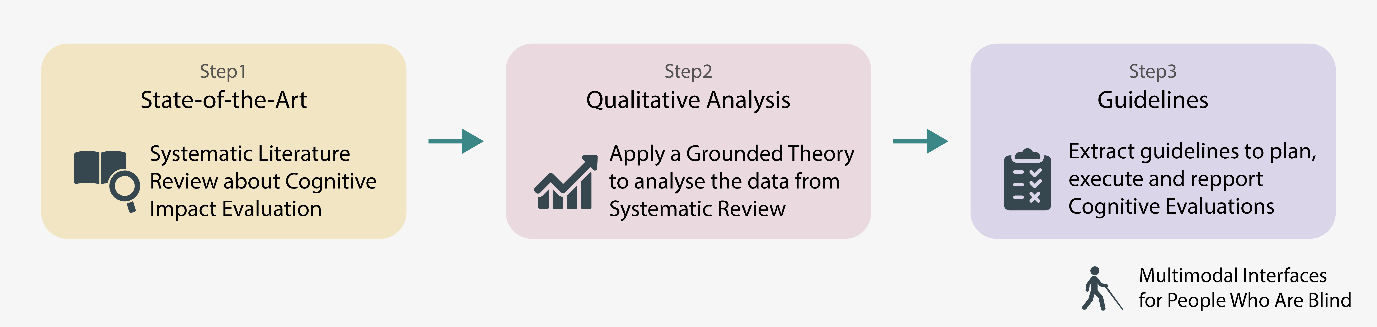
\includegraphics[width=16cm]{figuras/methodology.png}
		}{
			\Fonte{Produced by the author.}
		}	
	\end{figure}


\section{Document Organization}
\label{sec:introduction-organization}

The remainder of the document is organized as follows:
\begin{itemize}
    \item Chapter \ref{cap:background} – Theoretical Background: this chapter describes the bibliography used during the development of this research. This chapter presents the theoretical basis of assistive technology for people who are blind, multimodal interfaces, and \gls{EBSE}.
    \item Chapter \ref{chap:metodologia} – Methodology: this chapter presents the whole process proposed and applied to achieve our objective which is composed of two main steps: The Systematic Literature Review and the Grounded Theory process.
    \item Chapter \ref{chap:resultados} – Results: this chapter presents the results of each step of the methodology that answer the research questions and drives this work. The findings of the literature review and grounded theory process turned into guidelines after the analysis performed. 
    \item Chapter \ref{chap:guidelines} – Guidelines: the findings of the literature review and grounded theory process turned into guidelines after the analysis performed, which  supports cognitive impact evaluation in the context of this study.
    \item Chapter \ref{chap:conclusion} – Conclusion: this chapter presents the conclusion and outlines the main contributions of this research. Moreover, it presents some limitations and some possible paths for future work to continue the research herein presented.
\end{itemize}
	\chapter{Background}
\label{cap:background}

In this chapter, we present the main definitions and theoretical background based on the literature review to achieve the goal of the work. Section \ref{sec:background-technology} presents the blindness aspects and the assistive technology for this target users. Section \ref{sec:background-evidence-based} presents the evidence-based methods. Section \ref{sec:background-multimodal-interfaces} presents the multimodal concepts and concerns. Finally, Section
\ref{sec:background-cognitive-impact-evaluation} presents the main literature background on experiments from Cognitive Psychology and Software Engineering areas.

\section{Technology for people who are blind}
\label{sec:background-technology}
According to \citeonline{cook2008}, new technologies could contribute to the full inclusion of individuals who have disabilities in the mainstream of society. Software, mobile applications and IoT systems (Internet of Things) are powerful tools to provide assistive technologies as shown by many works \cite{AudioGene}\cite{2014213}\cite{Maike2016}.

Thus, the interface interaction should respect these requirements to improve the quality of user interaction for the growing population of people who are blind or visually impaired \footnote{The term ``people who are blind or visually impaired'' was derived from the People First Language to speak appropriately and respectfully about an individual with a disability.}. Some authors think that the user who is blind or visually impaired must be involved at all stages of design, research, and development of the technologies for them \cite{2012137}. For this, it is necessary to understand more about the disability, its characteristics, and causes, for example, the degree of vision loss. 

\subsection{Blindness}
\label{subsec:background-blindness}
The users with visual disabilities are very diverse regarding the degree of vision loss. There are levels of blindness and visual acuity that are defined by global organizations, as World Health Organization (\gls{WHO}). The most recent standard definitions from the International Classification of Diseases 11 \cite{WHO2018ICD} and published from World Health Organization (\gls{WHO}) classifies the severity of visual disability into six categories of visual acuity \cite{WHO2018Blindness}.

The categories of visual acuity are defined by testing the vision at 6 meters according to the Snellen chart Figure \ref{fig:snellen_chart}. This chart, first developed in 1862 by the Dutch ophthalmologist Hermann, is the most widely adopted tool visual acuity assessment \cite{Falkenstein2008}. Therefore, the visual acuity 6/18 means the person could see at 6 meters what the average person sees at 18 meters. The ``normal'' visual acuity is 6/6. Table \ref{tab:categories_of_visual_acuity} shows the categories defined. The term ``low vision'' is no longer used since the IDC International Classification of Diseases (ICD-10) \cite{WHO2018ICD}. It has been replaced by categories 1 and 2.

 	\begin{figure}[h] 
   	    \captionsetup{width=7cm}%Da mesma largura que a figura
		\Caption{\label{fig:snellen_chart} Snellen chart}
		\UFCfig{}{
			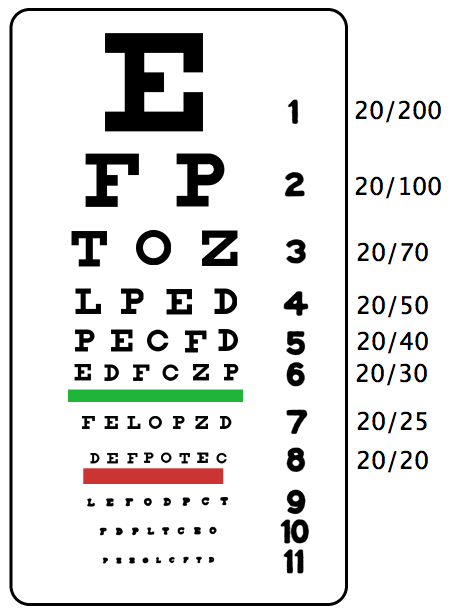
\includegraphics[width=7cm]{figuras/snellen_chart.png}
		}{
			\Fonte{\citeonline{Falkenstein2008}}
		}	
	\end{figure}
	
%jeff
\begin{table}[h]
	\captionsetup{width=13.5cm}%Deixe da mesma largura que a tabela
	\Caption{\label{tab:categories_of_visual_acuity} Categories of visual acuity}%
	\IBGEtab{}{%
		\begin{tabular}{m{6cm}m{3cm}m{3.2cm}}
			\toprule
			\multirow{2}{*}{Category} & \multicolumn{2}{c}{Presenting distance visual acuity} \\
			& Worse than & Equal to or better than\\
			\midrule \midrule
		    0 Mild or no visual impairment & & 6/18 \\			
			1 Moderate visual impairment & 6/18 & 6/60 \\
			2 Severe visual impairment & 6/60 & 3/60 \\
			3 Blindness & 3/60 & 1/60 \\
        	4 Blindness & 1/60 & Light perception \\
        	5 Blindness & No light perception & No light perception \\
			\bottomrule
		\end{tabular}%
	}{%
	\Fonte{\citeonline{WHO2018ICD}.}}
\end{table}	

According to the report Blindness and Deafness \cite{WHO2018Blindness}, the official descriptions of visual impairment and blindness of \gls{WHO} are:
\begin{quotation}
Visual impairment: Decrease or severe reduction in vision that cannot be corrected with standard glasses or contact lenses and reduces an individual’s ability to function at specific or all tasks.
Blindness: Profound inability to distinguish light from dark, or the total inability to see.
\end{quotation}

Each country has their definition of the term ``legally blind''. The United States of America, Canada, and most European countries define as the best-corrected visual acuity of 6/60 or worse in the better eye; and/or a visual field of 20 degrees or less. In Brazil, the ``legal blindnes'' definition only change in the numbers: visual acuity of 360 or worse and/or visual field of 60 degrees or less \cite{BRASIL1999DECRETO1999}.

We consider this work focused on people who are blind (levels 4 and 5 in Snellen chart), but which also consider people who are visually impaired (levels 1, 2 and 3 in Snellen chart) to have a broader view.

Other factors are also important to understand how the visual perception could influence the user interaction. Many works that evaluate technologies for people who are blind or visually impaired also examine as criteria related to vision impairment the age of blindness onset, the time with impairment \cite{Guerreiro2011} and the etiology of blindness (e.g., retinitis pigmentosa, glaucoma, Leber’s congenital amaurosis, retinopathy of prematurity) \cite{Connors2014} or visual impairment (e.g., glaucoma, age-related macular degeneration (AMD), corneal opacities, diabetic retinopathy, childhood blindness, trachoma, and onchocerciasis) \cite{WHO2018Blindness}.

The damage that prevented the vision could be produced by four sources: \textit{(i)} in transparent structures of the eye, such as cataracts and opacity of the cornea; \textit{(ii)} in the retina, such as macular degeneration and retinitis pigmentosa; \textit{(iii)} in the optic nerve, such as glaucoma or diabetes; and \textit{(iv)} in the brain. Blindness may be congenital or acquired. The damage that impedes vision can be caused at birth, at some event throughout the life of the individual or even in the womb.

\subsection{Assistive technology for people who are blind}
\label{subsec:background-assistive-technology}
Many applications areas have been developed to assist people who are blind or visually impaired. In this context, \citeonline{Manduchi2011} present four areas that have been produced research and technologies. The first one is \textit{mobility}, which provides a person who is blind moves safely, gracefully and comfortable, for example, avoiding obstacles. \textit{Wayfinding} promotes the capacity to know and track one’s position concerning the environment and find a route to a destination, for example, accessing spatial information from a distance. \textit{Printed information access} provides the vast printed information only accessible for sight, for example, read magazines. The last area is \textit{object recognition} that uses recognition algorithms to identify generic objects.

To illustrate these areas, see for instance some examples. Mobility and wayfinding areas are known as Orientation and Mobility (O\&M) \cite{Wiener2010,Welch2016}. In this area, the study \citeonline{Sanchez2014} presents the application Audiopolis (Figure \ref{fig:audiopolis}), a video game for navigating throw a virtual city interacting with audio and haptic interfaces. The Audiopolis also has the goal of improving evolving users' cognitive skills.

 	\begin{figure}[h] 
   	    \captionsetup{width=10cm}%Da mesma largura que a figura
		\Caption{\label{fig:audiopolis} A user playing Audiopolis}
		\UFCfig{}{
			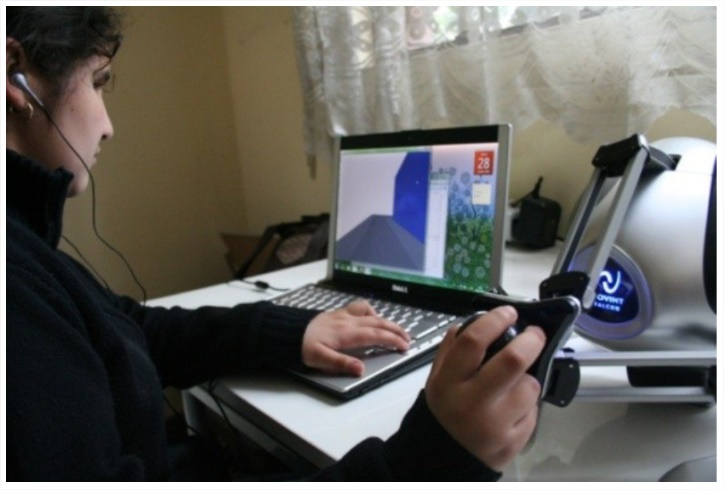
\includegraphics[width=10cm]{figuras/audiopolis.png}
		}{
			\Fonte{\citeonline{Sanchez2014}.}
		}	
	\end{figure}

In printed information access and object recognition areas, with a focus on approaches based on computer vision, the study \citeonline{Maike2016} presents the U-NEXT, an IoT system to perform the tasks of finding and selecting products in a supermarket by using RFID tags and audio feedback as output mode. Figure \ref{fig:U-NEXT} shows a possible scenario of the U-NEXT.

 	\begin{figure}[h] 
   	    \captionsetup{width=9cm}%Da mesma largura que a figura
		\Caption{\label{fig:U-NEXT} U-NEXT smart supermarket scenario}
		\UFCfig{}{
			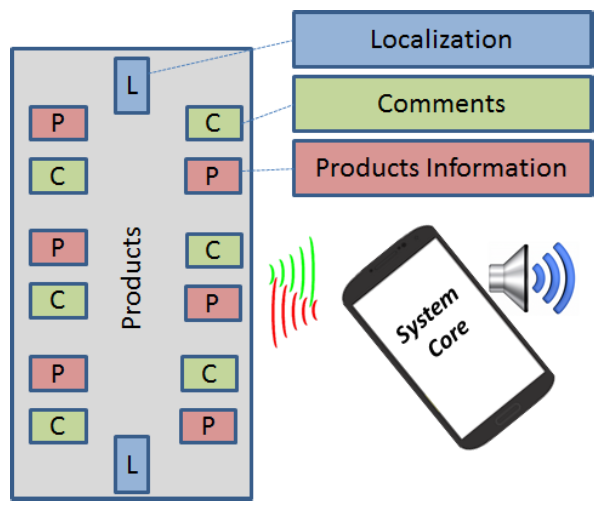
\includegraphics[width=9cm]{figuras/U-NEXT.png}
		}{
			\Fonte{\citeonline{Maike2016}.}
		}	
	\end{figure}

In the face of the large amount and kind of technologies that support the visually impaired and blindness disabilities, \citeonline{Pissaloux2018a} classify the devices that implement these technologies in two sorts: \gls{SSUD} (Sensory SUpplementation Devices) or \gls{SSD} (Sensory Substitution Devices), described as follows.
\begin{quotation}
\textit{\glspl{SSUD} aim to provide to the end user a complementary information which reinforces the user’s personal locomotion capacities and skills. Another sense(s)/modality(ies) are usually put to the contribution. This allows to provide subtle, user expected, cues which ensure that the user’s main attention is on the podo-tactile and auditory cues of the real world, and not on the locomotion cues of the device. Such cues may be exploited during a task execution \cite{Pissaloux2018a}.}

\textit{\glspl{SSD} aim to provide to the end user the information via another (substituting) sense; they offer a new language (new code) which should be learn independently of the initial (natural) role of this sense: a specific stimulus (a code) is associated with each object supposed to be perceived with a new sense \cite{Pissaloux2018a}.}
\end{quotation}

Considering the main objective of this work, we focus only on \gls{SSUD} (Sensory SUpplementation Devices) that includes computers, mobile devices, wearable devices, IoT systems or others according to the purpose of the application. The device \gls{SSD} (Sensory Substitution Devices), out of our scope, includes sensory replacement, haptics as sensory augmentation, bionic eyes, retinal visual prosthesis, cortical implants and others. This definition is important to plan the methodology used and to delimit the focus.

\section{Evidence-Based Software Engineering (\gls{EBSE})}
\label{sec:background-evidence-based}
The use of evidence-based strategies on software engineering has become more and more applied since the 1990s \cite{Shepperd2012}, and it was strongly influenced by clinical practice and the formation of medicine area. Before the research in software engineering is still too much of advocacy research and more scientific approach to software engineering is needed \cite{Wohlin2000}.

The evidence is used to prove the truth of some assertions. According to \citeonline{Shepperd2012}, empirical scientific evidence means that evidence has been obtained from observation (empirical) and in accordance with scientific principles as methods well known and it is documented in a complete and standard way. 

There are many forms for applying an empirical scientific evidence, for example, controlled experiments and quasi-experiments; case studies; surveys; action research and ethnography. Table \ref{tab:evidence_hierarchy} shows the evidence hierarchy considered in \citeonline{Shepperd2012}, helpful to appraising the value of empirical evidence.

\begin{table}[h]
	\captionsetup{width=16cm}%Deixe da mesma largura que a tabela
	\Caption{\label{tab:evidence_hierarchy} Evidence hierarchy}%
	\IBGEtab{}{%
		\begin{tabular}{m{2cm}m{4cm}m{4cm}m{4cm}}
			\toprule
			 & \textbf{Effectiveness} (how well does the intervention work?) & \textbf{Appropriateness} (how suitable is the intervention in the context) & \textbf{Feasibility} (the wider organizational issues of introducing the intervention) \\
			\midrule \midrule
			\textbf{Excellent} & Systematic review; Multi-centre study & Systematic review; Multi-centre study & Systematic review; Multi-centre study \\
			\textbf{Good} & RCT\footnote{RCT means Randomized Controlled Experiments}; Observational study & RCT; Observational study; Interpretive study & RCT; Observational study; Interpretive study \\
			\textbf{Fair} & Uncontrolled trial with dramatic results; Before/after study; Non-randomized controlled trial & Descriptive study; Focus group & Descriptive study; Action research; Before/after study; Focus group \\
			\textbf{Poor} & Descriptive study; Case study; Expert opinion; Poor quality study & Case study; Expert opinion; Poor quality study & Case study; Expert opinion; Poor quality study\\
			\bottomrule
		\end{tabular}%
	}{%
	\Fonte{\citeonline{Shepperd2012}.}%
%	\Nota{esta é uma nota, que diz que os dados são baseados na	regressão linear.}%
%	\Nota[Anotações]{uma anotação adicional, seguida de várias outras.}%
    }
    \end{table}

%%%Figura Excluídda e comentada %%%
\begin{comment}
 	\begin{figure}[h] 
   	    \captionsetup{width=16cm}%Da mesma largura que a figura
		\Caption{\label{fig:evidence_hierarchy} Evidence Hierarchy}
		\UFCfig{}{
			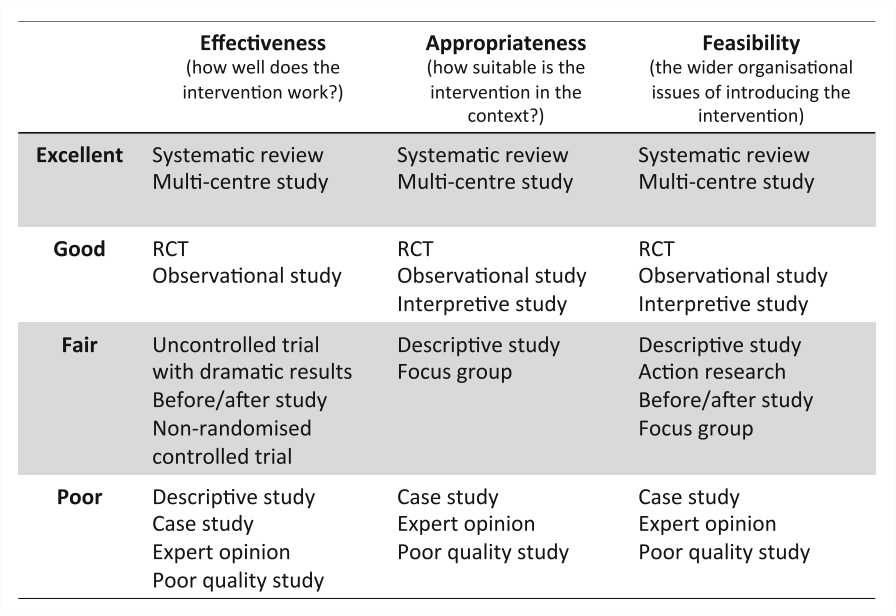
\includegraphics[width=16cm]{figuras/an_evidence_hierarchy_considered.png}
		}{
			\Fonte{\citeonline{Shepperd2012}.}
		}	
	\end{figure}
\end{comment}

\citeonline{Wohlin2000} consider three main empirical strategies in software engineering: \textit{(i)} setting up formal experiments; \textit{(ii)} studying real projects in industry, i.e., performing a case study; and \textit{(iii)} conducting surveys through, for example, interviews.

Considering the purpose of this work for evaluating the impact and effectiveness, we will focus on the experiment as the primary strategy to get evidence. Also, we explore surveys and case studies as empirical methods that have the same purpose. We expect to enable understanding and identification of relationships between different factors, or variables, that affect the use of technology for people who are blind or visually impaired. 

\section{Multimodal Interfaces}
\label{sec:background-multimodal-interfaces}
The perception of humans in their environment occurs through the five senses: vision, hearing, touch, taste, and smell. A mode or modality refers to receiving stimuli from one of these senses \cite{Turk2013}. The unimodal communication is not typical in the information exchange in the human communication. Usually, speech, gestures, facial expressions and others are used at the same time, as well when a person is speaking, he makes gestures to express better their feelings and emotions \cite{Turk2013}.

When a computational system works as multimodal interfaces, it enables the combination of multiple modes or channels of communication between the user and the device in the same interaction \cite{Oviatt2003}. These modes can be used sequentially or simultaneously and, in combination or independently, beyond the traditional input via keyboard and mouse, and monitor output \cite{Neto2008}. The use of multimodal interfaces increase the interaction quality as a result of \textit{(i)} supporting and accommodating the perceptive and communicative capacities of the users; and \textit{(ii)} integrating computational skills in the real world by offering more natural ways of interacting with humans \cite{Dumas2009}. According to \citeonline{Dumas2009} multimodal interfaces are:
Multimodal interfaces process two or more combined user input modes— such as speech, pen, touch, manual gestures, gaze, and head and body movements— in a coordinated manner with multimedia system output. They are a new class of interfaces that aim to recognize naturally occurring forms of human language and behavior, and which incorporate one or more recognition-based technologies (e.g., speech, pen, vision).

Such systems have the potential to function in a more robust and stable way than unimodal recognition systems involving a single interaction technology, such as speech, pen, or vision \cite{Oviatt2003}. \citeonline{Hauptmann1993} concluded that 71\% of the individuals surveyed prefer to use their hands and voice to control objects than a single isolated modality. Some studies seek to understand if the multimodal interaction is capable of facilitating user interaction with a computational system. Other works focus on specific combinations of input and output modes, for example, Interface Web/speech \cite{Neto2008}.

According to \citeonline{Dumas2009}, multimodal systems have the potential to improve Human-Computer Interaction in several ways, as increasing the robustness of systems combining different sources of information; flexible system customization, user-based and context-based; applicability in multi-user systems with mobile interaction; accessibility, since the system presents other alternative forms of interaction; ease of use of small and complex devices allowing more natural interaction in the execution of tasks \cite{InacioJunior2007}.

Inspired by Norman’s action cycle, \citeonline{Dumas2009} illustrates the model of multimodal man-machine communication (Figure \ref{fig:multimodal_man-machine_interaction}) with the major concepts that should be considered for multimodal systems: the fusion of multimodal inputs, and the multimodal fission to generate an adequate message to the user, according to the context of use, preferences and profile.

 	\begin{figure}[h] 
   	    \captionsetup{width=16cm}%Da mesma largura que a figura
		\Caption{\label{fig:multimodal_man-machine_interaction} Multimodal man-machine interaction}
		\UFCfig{}{
			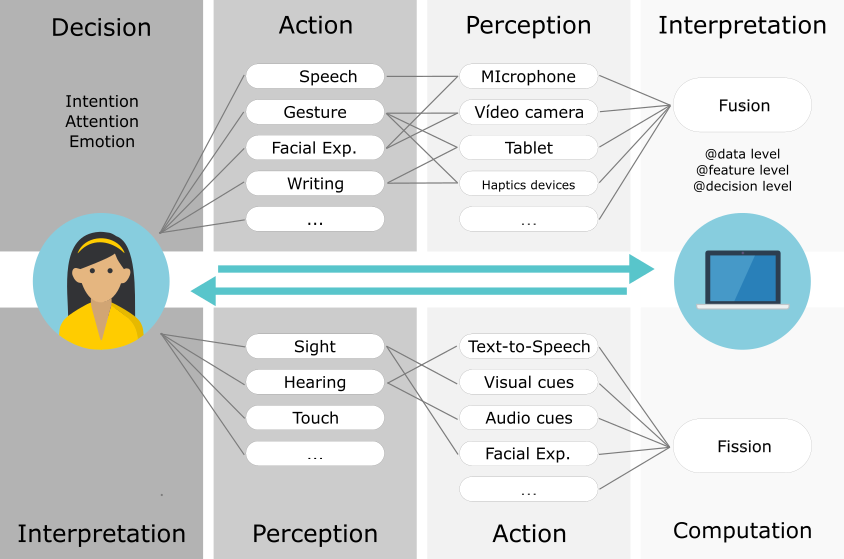
\includegraphics[width=16cm]{figuras/multimodal_man-machine_interaction.png}
		}{
			\Fonte{Adapted from \citeonline{Dumas2009}.}
		}	
	\end{figure}

This interaction between computer and human occurs in four states. On the user's side, the first is the decision state, where the content of the communication message is prepared consciously, intentionally or not, through attention and emotion. The second state is the state of action, where the media are selected, such as voice, gestures or facial expressions. On the computer side, the message is interpreted in the state of perception, where multimodal systems receive information from one or more sensors, at one or multiple levels of expression. In the state of interpretation, the system will attempt to give some meaning to the information received from the state of perception. This is typically the place where the merging of multimodal messages occurs. It is also in this state where the action is taken according to the system's business logic and defined management rule.
        
Depending on the meaning extracted in the interpretation, a response is generated and transmitted, which is where the fission occurs and determines the most relevant modalities for returning the message. This depends on the context of use, for example, within a car, and the user profile, for example, people who are blind.

Furthermore, the theory of processing the interaction requires mental resources at many stages, as shown in Human Information Processing system \cite{Lindsay1977}, described as a model by \cite{wickens2015engineering} as shown in Figure \ref{fig:human_information_processing}. In the Human Information Processing model, the information from the environment is firstly processed by our senses and after that as a Perception. Other elements involved are Attention, Long-term Memory, Working Memory Cognition, Response Selection, Response Execution, and the Feedback.

 	\begin{figure}[h] 
   	    \captionsetup{width=16cm}%Da mesma largura que a figura
		\Caption{\label{fig:human_information_processing} A model of human information processing}
		\UFCfig{}{
			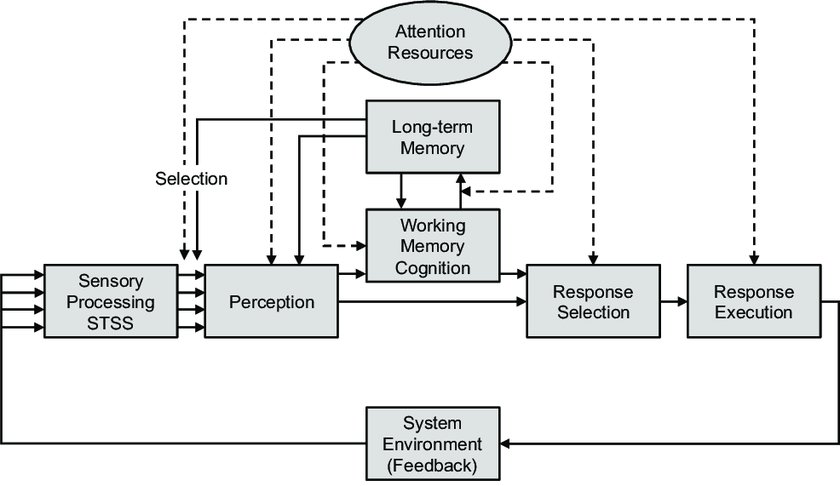
\includegraphics[width=16cm]{figuras/human_information_processing.jpg}
		}{
			\Fonte{\cite{wickens2015engineering}.}
		}	
	\end{figure}

Still related to the multimodal interaction, the proprioception sense could be considered to analyze the interaction on interfaces for people who are blind. The proprioception sense includes the sense of position and movement of our limbs, the senses of muscle force and effort, and the sense of balance \cite{proprioception}. Although it is related to interaction, this dissertation does not study this concept in depth.

Multimodal Interfaces for people who are blind can cover a wider range of users than traditional interfaces, including users of different ages, levels of knowledge, native languages, cognitive styles, impairments and other temporary illnesses or permanent physical disabilities, as well as visual impairment. In this area, blindness and visual impairments present challenges in most stages of human-computer interaction, from input actions, such as touch screen entry and cursor control, to perceiving output, such as interpreting a figure or a diagram \cite{Keates2015}.

While interfaces for the sighted user usually consist of mouse and keyboard as input, interfaces for users who are blind rely principally on auditory information, keyboards, and others haptic devices \cite{Sanchez2014a}. Replacing one mode on multimodal interfaces for another is not a simple solution. Nevertheless, many mobile accessibility solutions for people who are blind commonly replaces the onscreen information only for audio \cite{Guerreiro2011}. This proves that it is necessary to investigate the role of multimodal components in the development and evaluation, as done by \cite{Sanchez2015}. The impact of multimodal interfaces is also reviewed in \cite{Cao2010}, that shows the effect of multimodal interfaces in cognitive and emotional (stress) impact. 

This work aims to provide instruments to verify the real cognitive impact in multimodal interfaces on people who are blind or visually impaired considering the main aspects of multimodal interfaces.

\section{Cognitive Impact Evaluation}
\label{sec:background-cognitive-impact-evaluation}
There are technological aspects to these systems which are investigated from the perspective of how they affect use \cite{Ritter2014}. Cognitive impact concerns the interaction between humans and systems. The field of human-computer interaction has pioneered in the formal study of the cognitive relationship between a person's activities, the artifact of the computer, and the task \cite{Norman1986}. The technologies could enhance human cognitive capabilities. 

\citeonline{Darin2015} literature mapping study shows the cognitive process analyze applications according to a four-dimensional classification (Interface, Interaction, Cognition, and Evaluation). The evaluation dimension includes two main aspects: usability and cognitive impact. 

%\todo[inline]{RETIRADO - This last one assures that an application can develop or enhance any cognitive skills for people with visual disabilities.}

Still on this study, the cognition dimension comprises six skills: mental models, mental maps, spatial structures, Orientation and Mobility (O\&M), problem-solving, and social collaboration. Such approach addresses the main cognitive skills developed and enhanced for impact evaluation purposes. These dimensions could provide directions to define tasks in an experiment to measure the cognitive impact as detection of some obstacles, a useful data for evaluating O\&M \cite{Pissaloux2018a}. 

The study also shows that most papers classified in main cognitive skills are about Mental Map and O\&M. The O\&M skill is a broad concept that is also related to wayfinding and navigation. According to \citeonline{Pissaloux2018a}, ``Human mobility is one of the most important cognitive tasks. Indeed, independent and secure mobility in real physical space has a direct impact on the quality of life, on well-being, and on integration in the numeric society.''

\citeonline{Darin2017} define mobility in a four-dimensional problem: \textit{walking}, \textit{wayfinding} (or orientation), \textit{space awareness} (or space knowledge) and \textit{navigation}. According to this definition, walking is a low conscious cognitive task and involves displacement in the near space. It takes in account obstacle detection and localization. The wayfinding is a set of processes to know one’s current position in space to reach one’s target. The space awareness requires a high consciousness level. It includes forming mental maps, e.g., know the name of the street on a plan. The navigation, the highest-level cognitive task, is a result of the implementation of all listed above functions while traveling.

The impact evaluation of software could use several evidence-based methods. This work focuses on the experiments. To treat the cognitive impact evaluation is necessary to comprehend the experiment design in both cognitive psychology and software engineering areas. The two main theoretical background bibliography used in this work are the books ``Cognitive Psychology'' \cite{Sternberg2011} and ``Experimentation in Software Engineerin'' \cite{Wohlin2000}. In this multidisciplinary context, the next two subsections are dedicated to explain each point of view and highlights the differences. Aside from experiments, the cognitive workload could be measured by an instrument of evaluation, as the questionnaire Nasa-Task Load Index (NASA-TLX) \cite{Hart2006Nasa-TaskLater}, which is a multi-dimensional scale designed to obtain workload estimates from one or more operators while they are performing a task or immediately afterwards.

\subsection{Design experiment in software engineering}
\label{subsec:background-design-experiment-software-engineering}
The experiment process includes several steps: Scoping; Planning; Operation; Analysis and interpretation; Presentation and package \cite{Wohlin2000}. Figure \ref{fig:overview_of_the_experiment_process} presents an overview of the experiment process and artifacts produced. This process provides a high level of control, which uses a formal, rigorous and controlled investigation. Its steps were used to analyze the data of experiments in the methodology proposed (Chapter \ref{chap:metodologia}). Also, the guidelines proposed in this work have the attribute ``when'' that provides in which phase the guidelines are applied.

 	\begin{figure}[h] 
   	    \captionsetup{width=16cm}%Da mesma largura que a figura
		\Caption{\label{fig:overview_of_the_experiment_process} Overview of the experiment process}
		\UFCfig{}{
			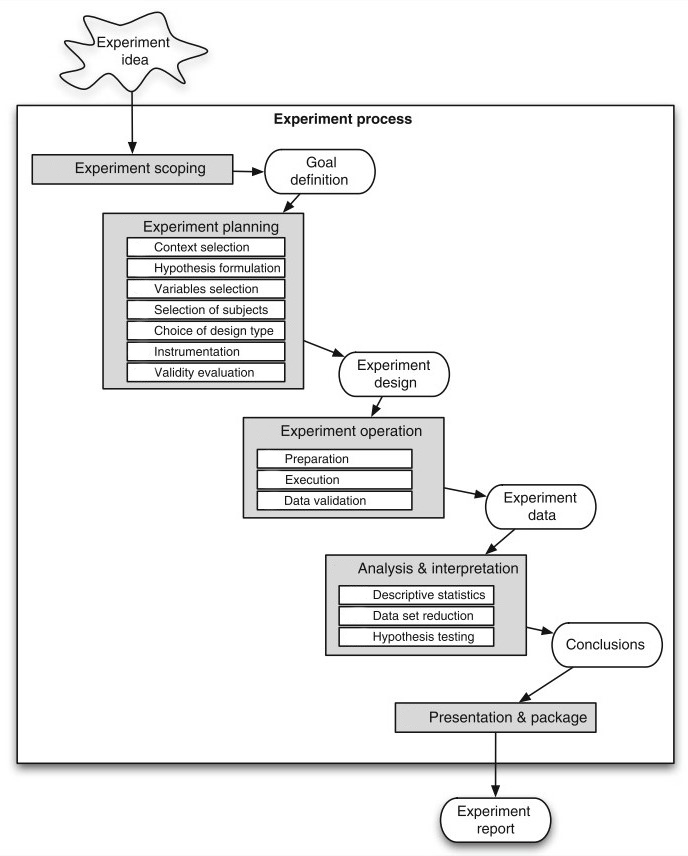
\includegraphics[width=16cm]{figuras/overview_of_the_experiment_process.png}
		}{
			\Fonte{Adapted from \citeonline{Wohlin2000}.}
		}	
	\end{figure}

The main concepts involved in the experiment, shown in Table \ref{tab:the_main_concepts_of_experimental_design}, are used to understand how the cognitive impact is evaluated and to conduct the designing of the guidelines. Figure \ref{fig:variable_relationship_in_the_experiment_process} shows how these concepts are related to the experimental process.

\begin{table}[h]
	\captionsetup{width=16cm}%Deixe da mesma largura que a tabela
	\Caption{\label{tab:the_main_concepts_of_experimental_design} The main concepts of experimental design}%
	\IBGEtab{}{%
		\begin{tabular}{m{2cm}m{13cm}}
			\toprule
			Concepts & Description \\
			\midrule \midrule
			Measure & A mapping from the attribute of an entity to a measurement value. \\
			Instrumentation & The instruments for an experiment are of three types, namely objects, guidelines and measurement instruments. \\
			Dependent Variables & The dependent variables are those we want to see the effect; the independent variables are those controlled and manipulated. \\
			Independent Variables & The independent variables are those controlled and manipulated. \\
			Factors & The independent variables which the experiment changes to verify the effect. Treatment is one value of a factor. \\
			\bottomrule
		\end{tabular}%
	}{%
	\Fonte{\citeonline{Wohlin2000}.}%
%	\Nota{esta é uma nota, que diz que os dados são baseados na	regressão linear.}%
%	\Nota[Anotações]{uma anotação adicional, seguida de várias outras.}%
    }
    \end{table}

 	\begin{figure}[h] 
   	    \captionsetup{width=16cm}%Da mesma largura que a figura
		\Caption{\label{fig:variable_relationship_in_the_experiment_process} Variable relationship in the experiment process}
		\UFCfig{}{
			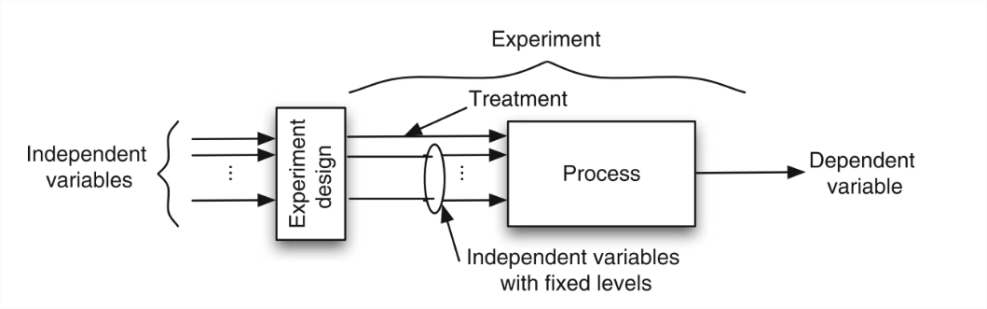
\includegraphics[width=16cm]{figuras/variable_relationship_in_the_experiment_process.png}
		}{
			\Fonte{\citeonline{Wohlin2000}.}
		}	
	\end{figure}

The treatments are measured in the dependent variable, often only one \cite{Wohlin2000}. The variable is mostly not directly measurable, and the experimenter have to measure it via an indirect. Wohlin defines measurement and measure as: ``measurement is the process by which numbers or symbols are assigned to attributes of entities in the real world in such a way as to describe them according to clearly defined rules''. A measure is the number or symbol assigned to an entity by this relationship to characterize an attribute.

As an example of experiment process, we consider the measurements, instrumentation, and variables from the experiment conducted in \citeonline{Connors2014}. In this study, the authors evaluate the navigational performance the of virtual environment called Audio-based Environment Simulator (AbES) that can be explored for the purposes of learning the layout of an unfamiliar, complex indoor environment. The dependent variable evaluated was the navigation performance (Orientation \& Mobility, O\&M).

Some information about the participants is controlled and works as independent variables such as etiology of blindness, age, gender, hand preference, and verbal memory (assessed by using the Wechsler Memory Scale). These variables are controlled and fixed to ensure the correct measurement. The factors in the experiment are the age of blindness onset and the interaction condition with AbES. The factors are randomly distributed into groups: early blind and late blind; and gamers, directed navigators, and control group. The measurements variables used are task success, navigation time, and shortest possible path score.

\subsection{Design experiment in Cognitive Psychology}
\label{subsec:background-design-experiment-cognitive-psychology}
The research methods to in Cognitive Psychology focuses on describing particular cognitive phenomena, such as how people preconceived notions regarding what they may find while gathering the data \cite{Sternberg2011}. To achieve the goal, the research should include more than one method. Among them, the literature present that cognitive psychologists use controlled experiments, psychobiological research, self-reports, case studies, naturalistic observation, and computer simulations and artificial intelligence when studying cognitive phenomena \cite{Sternberg2011}.

Focusing on controlled experiments, the Table \ref{tab:experiment_to_cognitive_phenomena} presents characteristics of controlled experiments to explore cognitive phenomena.

\begin{table}[h]
	\captionsetup{width=16cm}%Deixe da mesma largura que a tabela
	\Caption{\label{tab:experiment_to_cognitive_phenomena} Experiment to cognitive phenomena}%
	\IBGEtab{}{%
		\begin{tabular}{m{3cm}m{12cm}}
			\toprule
			 & Controlled Laboratory Experiments \\
			\midrule \midrule
			Description of method & Obtain samples of performance at a particular time and place. \\ \hline
			Random assignment of subjects & Usually. \\ \hline
			Experimental control of independent variables & Usually. \\ \hline
			Sample representativeness & May be any size. \\ \hline
			Ecological validity & Not unlikely; depends on the task and the context to which it is being applied. \\ \hline
			Information about individual differences & Usually de-emphasized.\\ \hline
			Strengths & Easy to administer, score, and do statistical analyses; High probability of drawing valid causal inferences.\\ \hline
			Weaknesses & Difficulty in generalizing results beyond a specific place, time, and task setting; Discrepancies between behavior in real life and in the laboratory.\\ \hline
			Examples & \citeonline{Karpicke2009} developed a laboratory task in which participants had to learn and recall Swahili-English word pairs. After subjects first recalled the meaning of a word, that pair was either dropped, presented twice more in a studyperiod, or presented twice more in test periods. Subjects took a final recall test one week later.\\ \hline
			\bottomrule
		\end{tabular}%
	}{%
	\Fonte{\citeonline{Sternberg2011}}%
%	\Nota{esta é uma nota, que diz que os dados são baseados na	regressão linear.}%
%	\Nota[Anotações]{uma anotação adicional, seguida de várias outras.}%
    }
    \end{table}

Regarding the experiment concepts, the variables of the experiment are \textit{(i)} independent variables, that are individually manipulated, or carefully regulated, by the experimenter; or \textit{(ii)} dependent variables, that are outcome responses, the values of which depend on how one or more independent variables influence or affect the participants in the experiment \cite{Sternberg2011}. This literature also presents the concepts of \textit{(iii)} irrelevant variables, which affect the outcomes (dependent variable) when manipulated; \textit{(iv)} control variables, which are held constant; and \textit{(v)} confounding variables, which affect the dependent variables without be controlled or manipulated and should be avoided. 

Independent and dependent variables must be chosen with great care, because what is learned from an experiment will depend almost exclusively on the variables one chooses to isolate from the often complex behavior one is observing \cite{Sternberg2011}. The authors suggest two dependent variables that are used in cognitive-psychological research: percent correct (or its additive inverse, error rate) and reaction time. These measures are popular because they can tell the investigator, respectively, the accuracy and speed of mental processing \cite{Sternberg2011}. 

Among the myriad possibilities for independent variables are characteristics of the situation, of the task, or of the participants \cite{Sternberg2011}. For example, characteristics of the situation may involve the presence versus the absence of particular stimuli or hints during a problem-solving task, as virtual versus real navigation \cite{Lahav2008b}. Characteristics of the task may involve reading versus listening to a series of words and then responding to comprehension questions. Characteristics of the participants may include age differences, differences in educational status, or differences based on test scores. Characteristics of the participant are not easily manipulated experimentally due to the ethical regulation.
	\chapter{Methodology}
\label{chap:metodologia}

In this chapter, we present the research methodology which is composed of three steps: the literature review, the Grounded Theory. Section \ref{sec:methodology-overview} gives an overview of the research methodology. Section \ref{sec:methodology-slr} explains the Systematic Literature Review process. Section \ref{sec:methodology-gt} shows how the Grounded Theory method was applied.


\section{Overview}
\label{sec:methodology-overview}
The methodology consists of three steps: \textit{State-of-the-Art}, \textit{Qualitative Analysis}, and the \textit{Guidelines} formulation. The Systematic Literature Review of the State-of-the-Art step aims to review the existing evidence concerning the impact evaluation of multimodal interfaces and seeks to summarize the empirical evidence concerning the strengths and limitations of a specific evaluation method \cite{Kitchenham2007}. In Qualitative Analysis, the Grounded Theory \citeonline{Glaser1967} builds a theory of cognitive impact evaluation from data retrieved in the Systematic Literature Review. After, we offer guidelines based on all data analyzed and the discussion of weak points encountered of cognitive impact evaluation of multimodal interfaces for people who are blind or visually impaired. 


\section{Systematic Literature Review}
\label{sec:methodology-slr}
In contrast to an ad-hoc literature review, the systematic literature review is a methodologically rigorous analysis and study of research results. To achieve our goal, the main research question for this first part of the proposal was \textbf{``How is the cognitive impact evaluated on multimodal interfaces for people who are blind''}. For a better understanding, as a second goal question, we aim to learn the challenges regarding impact evaluation on this scenario.

The process of a systematic literature review includes three main phases: planning the review; conducting the review and reporting the review \cite{Kitchenham2007}. During all process of the systematic literature review, we used the tool StArt (``StArt'', 2016) and the software Microsoft Excel\footnote{Microsoft Excel - \url{https://products.office.com/pt-br/excel}} as a support to create the protocol, apply the filters, select the papers and show the results. We organize all references on software Mendeley\footnote{Mendeley - \url{https://www.mendeley.com/}}. As the papers retrieved from PubMed Central are in MEDLINE format, we developed the tool Medline2bibtex\footnote{Medline2Bibtex - \url{https://github.com/lanabia/Medline2Bibtex}}. It works as a parser to permit the list to be read by both StArt and Mendeley.

Each of these stages has a qualitative methodological design that aims to offer a better specification and evolution in the development of the systematic literature review. Figure \ref{fig:systematic_literature_review} presents the SLR process adopted in this study by using a UML language\footnote{UML - \url{http://www.uml.org/}} for Activity Diagram. The process suits the guidelines from \cite{Kitchenham2007}. The next subsections describe the planning (the study selection criteria, the research sources selected) and the conducting phase (the search Process, the data extraction form fields and the studies quality evaluation). The entire process was stored in an excel worksheet available online\footnote{\url{https://www.dropbox.com/s/dvvn44cymqsqguy/Systematic\%20Review\%20-\%20Mesquita\%20L.\%202018.xlsm?dl=0}}.

 	\begin{figure}[h] 
   	    \captionsetup{width=16cm}%Da mesma largura que a figura
		\Caption{\label{fig:systematic_literature_review} Systematic Literature Review Process}
		\UFCfig{}{
			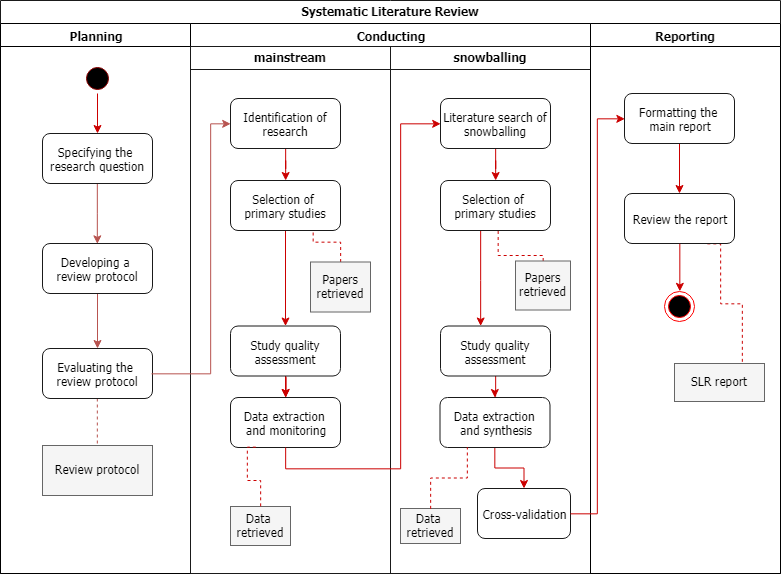
\includegraphics[width=16cm]{figuras/systematic_literature_review.png}
		}{
			\Fonte{Produced by the author based on \citeonline{FACANHA2018}.}
		}	
	\end{figure}

\subsection{Planning: definition of the protocol}
\label{subsec:methodology-planning}

In the planning phase, we define a review protocol that specifies the research question being addressed and the methods that will be used to perform the review \cite{Kitchenham2007}. The overall goal of this systematic literature review is to analyze the state-of-the-art and the study opportunities related to the cognitive impact evaluation of multimodal interfaces for people who are blind. Then, we addressed the following main and second questions.

    \begin{itemize}
        \item \textbf{Main question}: How is the cognitive impact evaluated on multimodal interfaces for people who are blind?

        \item \textbf{Second question}: Which are the challenges regarding impact evaluation on this scenario?
    \end{itemize}
    
\textbf{Sources selection}

The first suggested digital libraries as sources are: \textit{ACM Digital Library}; \textit{Engineering Village}; \textit{IEEE Xplore}; \textit{Scopus}; \textit{Science Direct}; \textit{Springer Link}; \textit{PubMed}; \textit{Web of Science}; \textit{Google Scholar}, that includes the leading conferences and journals from Computer Science.

The bases chosen are the primary research bases for scientific articles in the research area or the bases that index them. Since Scopus, which index ACM Digital Library and IEEE Xplore, is based on the same database of ScienceDirect. So, we choose Scopus that is considered the most effective search engine \cite{Burnham2006}. 

We withdrew Engineering Village because their twelve engineering document databases covered do not cover the content of this research. Scopus and Web of Science do not have the same database \cite{Tober2011}, so we maintain these two in the final source list. As the research include visual disabilities, we expect to find some works in PubMed database.

Although Google Scholar is declared as a credible alternative at the same level of Scopus in the face of the Web of Science \cite{Harzing2016}, it is not considered as a database, and it is only considered as a search engine. The final list of sources to systematic literature review is \textit{Scopus}, \textit{Springer}, \textit{Web of Science} and \textit{PubMed Central}.

We also research in the Journal of Visual Impairment \& Blindness that addresses a variety of topics related to visual impairment. The research in this journal changes a little the string applied to get their proceedings, that are in the scientific base PubMed Central.

\textbf{Studies initial selection}

The initial selection occurs by applying a search string into in each source. Before the final version of the string, we simulated many other strings in searching the best solution and results with the principal papers of the area, covering a broad range of possible papers in the search criteria. The final string defined was the string bellow.

The string will be applied on the metadata of papers, that includes abstract, index terms, and bibliographic citation data (such as document title, publication title, etc.). The research in the sources are applied by using the research string and the two initial criteria: to be published after 1998 and to be written in English. Based on the goal of systematic literature review we define the search string as shown in the Figure \ref{fig:string}.

 	\begin{figure}[h] 
   	    \captionsetup{width=14cm}%Da mesma largura que a figura
		\Caption{\label{fig:string} Search string}
		\UFCfig{}{
			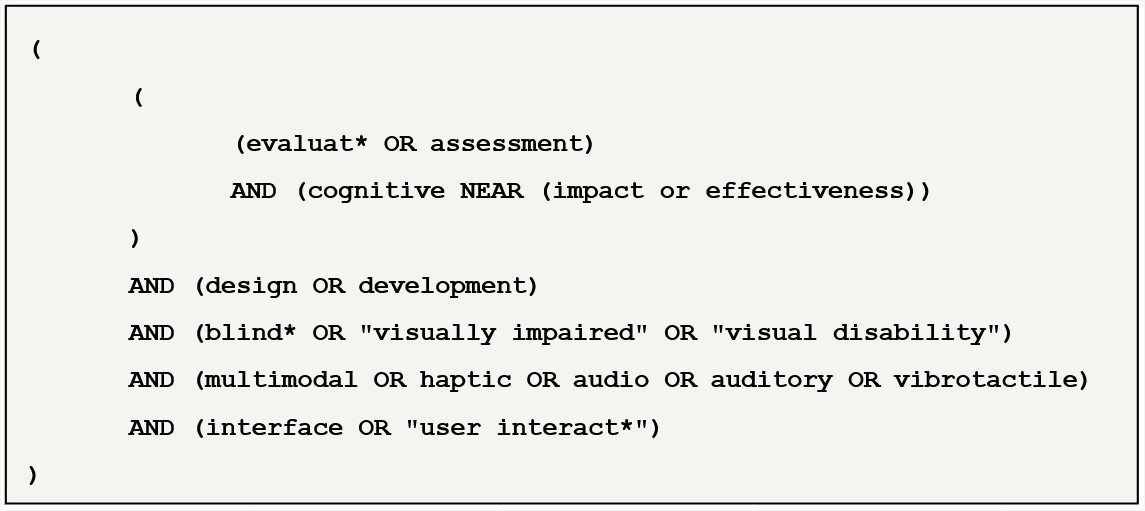
\includegraphics[width=14cm]{figuras/string.jpg}
		}{
			\Fonte{Produced by the author.}
		}	
	\end{figure}

%%Nao ficou legal em código, mas deixei ai caso vc queira testar%%
%\begin{lstlisting}[]
%(
%    (
%     (evaluat* OR assessment)
%     AND ((cognitive OR psychomotor OR physical OR emotional)
%                (NEAR/10 (impact or effectiveness))
%    )
%    AND (design OR development)
%    AND (blind* OR "visually impaired" OR "visial disability")
%    AND (multimodal OR hapatic OR audio OR auditory OR vibrotactile)
%    AND interface
%)
%\end{lstlisting}

\textbf{Study selection criteria}

We define the search criteria as studies that present technology for people who are blind or visually impaired and has applied a cognitive impact evaluation. The inclusion and exclusion criteria are according to the goal of the systematic literature review. These requirements comply the general objective of this study, but also aim to have a broader view of the assessment in various technologies in the area. Table \ref{tab:inclusion_and_exclusion_criteria} presents the inclusion \textit{(I)} and exclusion \textit{(E)} selection criteria. To be accepted, a scientific paper must cover all inclusion criteria and none exclusion criterion.

\begin{table}[h]
	\captionsetup{width=16cm}%Deixe da mesma largura que a tabela
	\Caption{\label{tab:inclusion_and_exclusion_criteria} Inclusion and exclusion criteria}%
	\IBGEtab{}{%
		\begin{tabular}{m{1cm}m{6cm}m{1cm}m{6cm}}
			\toprule
			Code & Inclusion Criteria & Code & Exclusion Criteria \\
			\midrule \midrule
			I.01 & The study has the technology for people who are blind or visually impaired & E.01 & Title and abstract out the search criteria (I.02, I.03, I.04) \\
			I.02 & The study evaluates the technology by using some approach that involves the user & E.02 & Entire text out the search criteria (I.02, I.03, I.04) \\
			I.03 & The study evaluates the technology by using a method to evaluate the cognitive impact & E.03 & The document is a book, a congress’ abstract, an extended abstract, a poster, an oral communication, proceedings of a conference, a seminar, a research plenary, a dictionary or an encyclopedia \\
			 & & E.04 & The study must be published after 1998 and written in English \\
			\bottomrule
		\end{tabular}%
	}{%
	\Fonte{Produced by the author.}%
%	\Nota{esta é uma nota, que diz que os dados são baseados na	regressão linear.}%
%	\Nota[Anotações]{uma anotação adicional, seguida de várias outras.}%
    }
    \end{table}

The technologies defined in the \textit{I.01} criterion include mobile application, computer software, IoT systems, virtual environments or a video game with multimodal interfaces. Also, we accept technologies that are not specifically for people who are blind or visually impaired with the goal of expanding the results, but the studies present the technology focused on users with visual disabilities. We exclude from all technologies that uses Sensory Substitution Devices \cite{Pissaloux2017TowardsDevices}, which substitutes a sense. The device SSD (Sensory Substitution Devices), out of our scope, includes sensory replacement, haptics as sensory augmentation, bionic eyes, retinal visual prosthesis, cortical implants and others. This definition is important to plan the methodology proposed and to delimit the focus.

We define the studies type in the \textit{E.03}. This criterion excludes all studies type different from primary studies that present technology for people who are blind and its evaluation. We accept papers of journals, conference papers, short papers, and book chapters. This criterion includes documents that have the minimum information to understand the evaluation. We did not cover books because the information is dispersed inside them.

The \textit{E.04} criterion defines the scientific articles must be in English, because it is the mandatory language for the main events and scientific journals in the search area. And they must be published between 1st January 1998 and 2nd August 2017. The year 1998 was a milestone due to the paper \citeonline{Lumbreras1998} which works with 3D acoustic interfaces for blind children and is the last study known.

To be accepted, a scientific paper must be covering all inclusion criteria and none exclusion criterion, as shown in the follow logical equation \ref{eq:logical}:

 \begin{equation}
    \label{eq:logical}
	((I.01)\wedge(I.02)\wedge(I.03))\vee(E.01)\vee(E.02)\vee(E.03)\vee(E.04)
 \end{equation}


\subsection{Conducting}
\label{subsec:methodology-conducting}

In the conducting phase, firstly, we identify and select studies. To identify, we did a manual string research in five scientific bases: Scopus, Springer Link, PubMed, PubMed Central, and Web of Science. We chose the main research bases in the research area or the bases that index them (HARZING; ALAKANGAS, 2016). Other bases were not included because they are indexed by the bases considered.

\subsubsection{Search Process}
\label{subsubsec:methodology-conducting-search}

The conducting phase starts with the initial search in the scientific bases proposed. The string was applied on the metadata of papers, which includes abstract, index terms, and bibliographic citation data (such as document title, publication title, etc.). It was retrieved 2136 papers. Figure \ref{fig:filters} presents the filters.

 	\begin{figure}[h] 
   	    \captionsetup{width=16cm}%Da mesma largura que a figura
		\Caption{\label{fig:filters} Filters in the conducting phase}
		\UFCfig{}{
			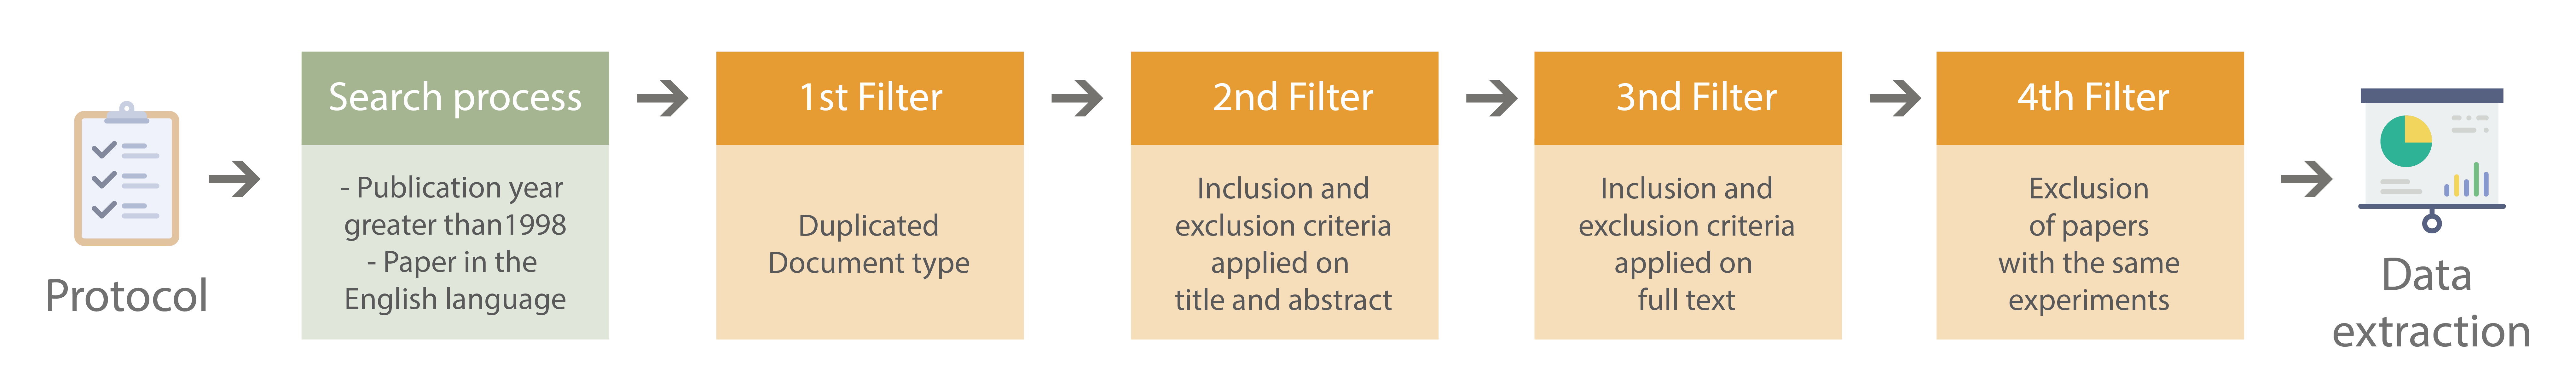
\includegraphics[width=16cm]{figuras/filters.png}
		}{
			\Fonte{Produced by the author.}
		}	
	\end{figure}
	
The first filter excluded papers duplicated and document types out the scope due their format (\textit{E.03}). The second filter identifies which paper is in and out the scope by reading their titles and abstracts (\textit{E.01}). A lot of papers were excluded in the first filter because the scientific base PubMed Central (PMC) brings a lot of medical papers focused on disease effectiveness and specific medical statements. Even though the area of this study is computer science, we decided to insert the PMC in the bases’ list due to the nature of the subject. 

Next, in the third filter, we evaluated each retrieved paper in its entirety (\textit{E.02}). If necessary, besides the entire text, we search more about the technologies and processes described, as project and institutional websites, videos, newspaper articles and others. In the fourth filter, we search and compare the experiments to find the same experiment described in two or more papers. This occurs when the experiment is not the primary goal of the paper, and more than one paper cites the experiment methodology and results according to the paper goal.

Once we have chosen the select papers, we extract all data required to achieve the objective. The organization of the data generates data synthesis, which will be shown in the Section \ref{sec:results-empirical}. The main reason for withdrawing papers in the last filter was the evaluation performed is out the search and at most times related to the system performance, e.g., sensor performance evaluation. 

In face the final papers selected, we make a snowballing approach for an opportunistic search for other relevant papers. Snowballing is a manual search using the reference and citations (known as backward and forward snowballing) list of a paper or the citations to the paper select aiming to identify additional papers \cite{Wohlin2014}. Thus, we perform other interaction among the forward and backward snowballing list to select the papers reading the title firstly and abstract and after the whole text. The only interaction of both snowballing processes is due to the resource limitation and the number of papers excluded in the first filter of these papers, that eliminates duplicated papers and unwanted document types.


In the snowballing process, the acceptance rate was high compared to the mainstream search. This acceptance rate is due to the purchased papers are closely related to the theme of tools for people who are blind and usually use similar processes of validation building.


% \subsubsection{Cross-validation}
% \label{subsubsec:methodology-cross-validation}

% The cross-validation process is used to create a protection mechanism to reduce the bias \cite{Kitchenham2007}. We invited 5 specialists on systematic literature reviews and software engineering and asked them to validate a sort of 10 papers among 20 offered, which we choose randomly from 195 papers selected in the second filter. We use their selection result to compare with our and to get the accuracy of the filter. 

% In this cross-validation, we are testing the third filter of the systematic literature review, on which we read the entire papers to select them regarding the inclusion criteria. For this reason, the form does not take account in exclusion criteria, and it takes only on inclusion criteria. Figure \ref{fig:cross_validation} shows the cover of cross-validation form which is available online\footnote{\url{https://lana184.typeform.com/to/Y604av}}.

%  	\begin{figure}[h] 
%   	    \captionsetup{width=14cm}%Da mesma largura que a figura
% 		\Caption{\label{fig:cross_validation} Cross-validation form}
% 		\UFCfig{}{
% 			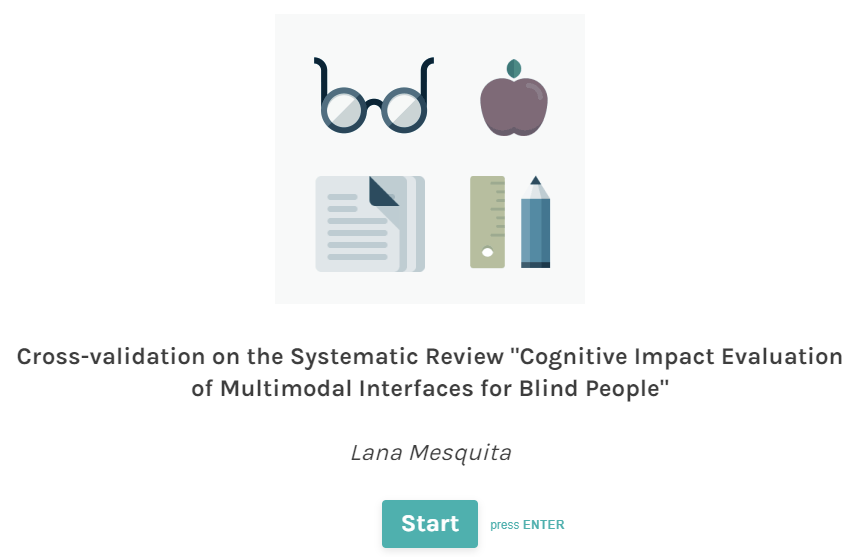
\includegraphics[width=14cm]{figuras/cross_validation.png}
% 		}{
% 			\Fonte{Produced by the author.}
% 		}	
% 	\end{figure}


\subsubsection{Studies quality evaluation}
\label{subsubsec:conducting-quality}

The quality evaluation for each paper accepted was based on the quality assessment in Table \ref{tab:quality_question} from \citeonline{Santos2017a}. Although the areas are different, the adaptations resulted in the following quality checklist to assess the studies and measure the weight of each study found on the results.

\begin{table}[h]
	\captionsetup{width=16cm}%Deixe da mesma largura que a tabela
	\Caption{\label{tab:quality_question} Quality assessment form}%
	\IBGEtab{}{%
		\begin{tabular}{m{1cm}m{14cm}}
			\toprule
			 & Quality Question \\
			\midrule \midrule
			\textbf{Q1} & Was it possible to extract all data regarding the data the Key features in multimodal interfaces (-0.1 pt per missing input; min value: -4.1 pts) \\
			\textbf{Q2} & Is there a complete description of how the evaluation has been applied? (1.0 pt per complete input in Empirical category; max value: 8,0 pts) \\
			\textbf{Q3} & Are the groups of participants in the experiment randomly assigned? (0.5 pt) \\
			\textbf{Q4} & Is the description of the impact evaluation understandable? (0.5 pt) \\
			\textbf{Q5} & Does the article present different evaluation types of the proposal? (1 pt) \\ 
			\textbf{Q6} & How many experiments does the paper present? (0.5 pt per experiment, if more than two experiments) \\
			\textbf{Q7} & Is the goal of the evaluation cleared defined? (0.5 pt) \\
			\textbf{Q8} & Is the hypothesis (null and alternative) explicitly described in the study? (0,5 pt) \\
			\bottomrule
		\end{tabular}%
	}{%
	\Fonte{Based on \citeonline{Santos2017a}.}%
%	\Nota{esta é uma nota, que diz que os dados são baseados na	regressão linear.}%
%	\Nota[Anotações]{uma anotação adicional, seguida de várias outras.}%
    }
    \end{table}

\subsubsection{Data Extraction Form Fields}
\label{subsubsec:methodology-data-extraction}

The data extraction was designed to answer the main and second questions and to understand the context in which each paper is inserted. We divide the data collected into three categories: \textit{(i)} General, \textit{(ii)} Research and \textit{(iii)} Empirical. The general category comprises bibliographic information. Table \ref{tab:data_collected} shows the data extracted and the categories.

\begin{table}[h]
	\captionsetup{width=13.2cm}%Deixe da mesma largura que a tabela
	\Caption{\label{tab:data_collected} Form for data collection}%
	\IBGEtab{}{%
		\begin{tabular}{m{1.2cm}m{10cm}m{1cm}}
			\toprule
			Category & Attribute & Type \\
			\midrule \midrule
			\multirow{7}{5em}{General} & Title & Text \\
			& The author(s) and affiliation & Text \\
			& The paper was published in a Journal, a Conference or as a Book chapter? & List \\
			& Year of publication & Number \\
			& Research type & List \\ 
			& Empirical Methods classification & List \\
			& Technologies the paper presents for people who are blind & Text \\ \hline
			\multirow{2}{5em}{Research} & Key features in multimodal interface & Text \\
			& Other strategies used to evaluate the interface (e.g. usability evaluation) & Text \\ \hline
			\multirow{8}{5em}{Empirical} & Sample & Text\\
			& Instruments & Text\\
			& Variables in the experimental design & Text\\
			& Statistical methods used & Text\\
			& Tasks defined & Text\\
			& Investigation cost (resources as time) & Text\\
			& Ethical concepts treated & Text\\
			\bottomrule
		\end{tabular}%
	}{%
	\Fonte{Produced by the author.}%
%	\Nota{esta é uma nota, que diz que os dados são baseados na	regressão linear.}%
%	\Nota[Anotações]{uma anotação adicional, seguida de várias outras.}%
    }
    \end{table}

The general category comprises bibliographic information and classifies the papers. We classified the  experiment of a scientific paper into two classifications: research type (Table \ref{tab:research_type_facet}), based on \citeonline{Petersen2008}. The research type is based on \citeauthor{Petersen2008} (\citeyear{Petersen2008}), which can be validation research, evaluation research, solution research, philosophical research, opinion paper or experience papers. The empirical method classification (Table \ref{tab:empirical__methods}) is based on the classification of \cite{Ampatzoglou2010}. This classification aims to confirm the papers retrieved are in the search focus, since we look for papers in the ``evaluation research'' type and that are ``Experiments''. Although, we retrieved one paper as a Case Study. For this one, we consider only the experiment data. All papers retrieved are in Evaluation Research category. 

\begin{table}[h]
	\captionsetup{width=16cm}%Deixe da mesma largura que a tabela
	\Caption{\label{tab:research_type_facet} Research type facet}%
	\IBGEtab{}{%
		\begin{tabular}{m{3cm}m{12cm}}
			\toprule
			Category & Description \\
			\midrule \midrule
			Validation Research & Techniques investigated are novel and have not yet been implemented in practice. Techniques used are for example experiments, i.e., work done in the lab. \\
			Evaluation Research & Techniques are implemented in practice and an evaluation of the technique is conducted. That means, it is shown how the technique is implemented in practice (solution implementation) and what are the consequences of the implementation in terms of benefits and drawbacks (implementation evaluation). This also includes to identify problems in industry. \\
			Solution Proposal & A solution for a problem is proposed, the solution can be either novel or a significant extension of an existing technique. The potential benefits and the applicability of the solution is shown by a small example or good line of argumentation. \\
			Philosophical Papers & These papers sketch a new way of looking at existing things by structuring the field in form of a taxonomy or conceptual framework. \\
			Opinion Papers & These papers express the personal opinion of somebody whether a certain technique is good or bad, or how things should been done. They do not rely on related work and research methodologies. \\ 
			Experience Papers & Experience papers explain on what and how something has been done in practice. It has to be the personal experience of the author. \\			\bottomrule
		\end{tabular}%
	}{%
	\Fonte{\citeonline{Petersen2008}.}%
%	\Nota{esta é uma nota, que diz que os dados são baseados na	regressão linear.}%
%	\Nota[Anotações]{uma anotação adicional, seguida de várias outras.}%
    }
    \end{table}
%%%Figura excluídda e comentada %%%
\begin{comment}
 	\begin{figure}[h] 
   	    \captionsetup{width=16cm}%Da mesma largura que a figura
		\Caption{\label{fig:research_type_facet} Research type facet}
		\UFCfig{}{
			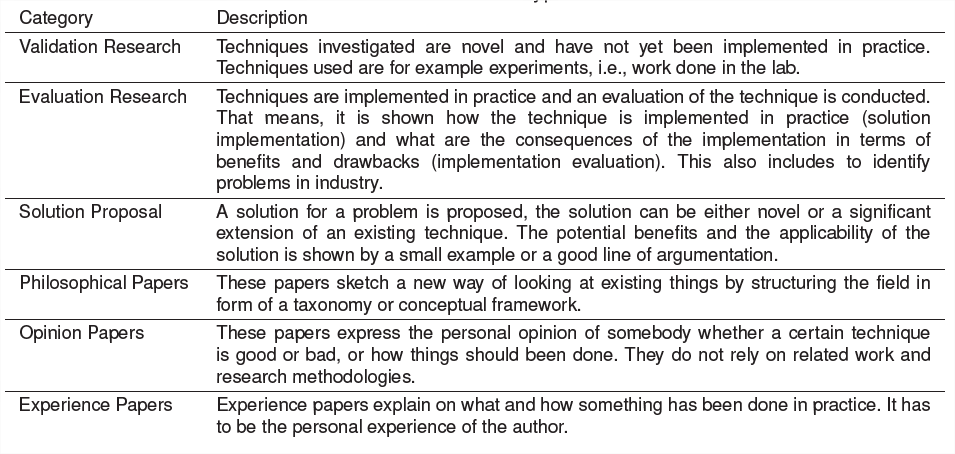
\includegraphics[width=16cm]{figuras/research_type_facet.png}
		}{
			\Fonte{\citeonline{Petersen2008}.}
		}	
	\end{figure}
\end{comment}

\begin{table}[h]
	\captionsetup{width=16cm}%Deixe da mesma largura que a tabela
	\Caption{\label{tab:empirical__methods} Empirical methods}%
	\IBGEtab{}{%
		\begin{tabular}{m{3cm}m{12cm}}
			\toprule
			Empirical method & Description \\
			\midrule \midrule
			Experiment & A set of a subjects is asked to perform a task in a highly controlled environment. the results are derived from observing of the subjects during the experiment, from inspecting the task outcome or from questioning the subjects at the end of the procedure.\\
			Survey & A set of subjects is asked to fill-in questionnaires either directly, or via internet. The results are derived from the valid answers to the questionnaire. \\
			Case study & A project, an activity or an assignment is monitored with respect to the methodology under study. Results are directly derived from project measurements. \\  \bottomrule
		\end{tabular}%
	}{%
	\Fonte{\citeonline{Ampatzoglou2010}.}%
%	\Nota{esta é uma nota, que diz que os dados são baseados na	regressão linear.}%
%	\Nota[Anotações]{uma anotação adicional, seguida de várias outras.}%
    }
    \end{table}

%%%Figura excluídda e comentada %%%
\begin{comment}
 	\begin{figure}[h] 
   	    \captionsetup{width=16cm}%Da mesma largura que a figura
		\Caption{\label{fig:empirical__methods} Empirical methods}
		\UFCfig{}{
			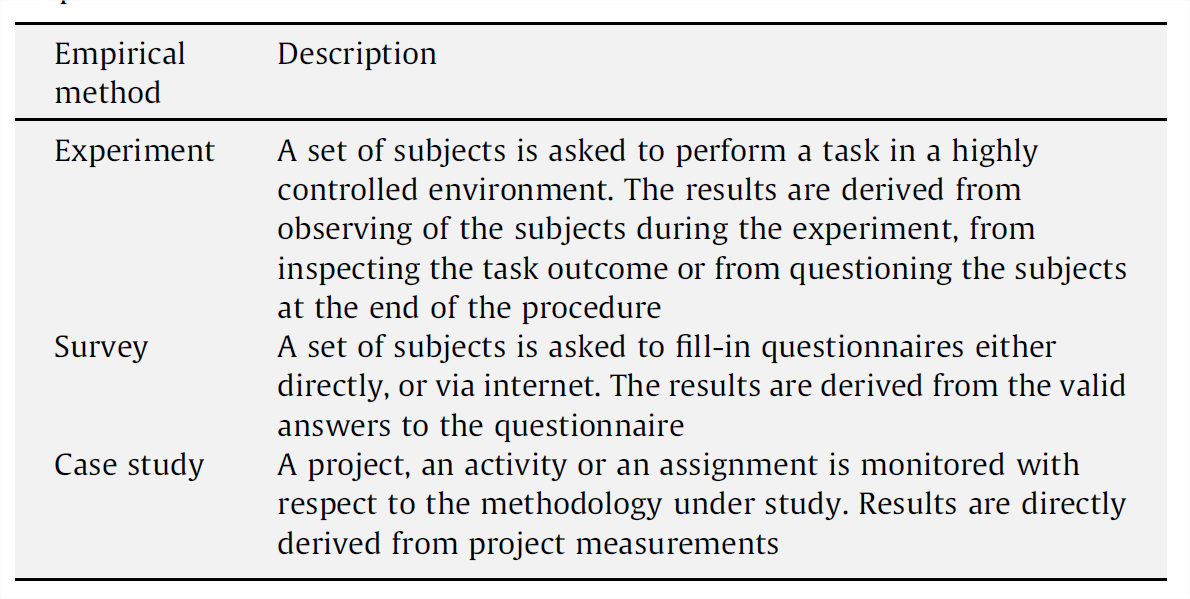
\includegraphics[width=16cm]{figuras/empirical__methods.png}
		}{
			\Fonte{ \citeonline{Ampatzoglou2010}.}
		}	
	\end{figure}
\end{comment}

The research category comprises the classification that fits the technology presented in the key features of multimodal interfaces for the cognition of people who are blind \cite{Darin2015}. This classification is divided into 4-dimension: Interface, Interaction, Cognition, and Evaluation; and it is applied to video games and virtual environments (Figure \ref{fig:key_features_multimodal_interfaces}).

 	\begin{figure}[h] 
   	    \captionsetup{width=14cm}%Da mesma largura que a figura
		\Caption{\label{fig:key_features_multimodal_interfaces} Key features in multimodal interfaces}
		\UFCfig{}{
			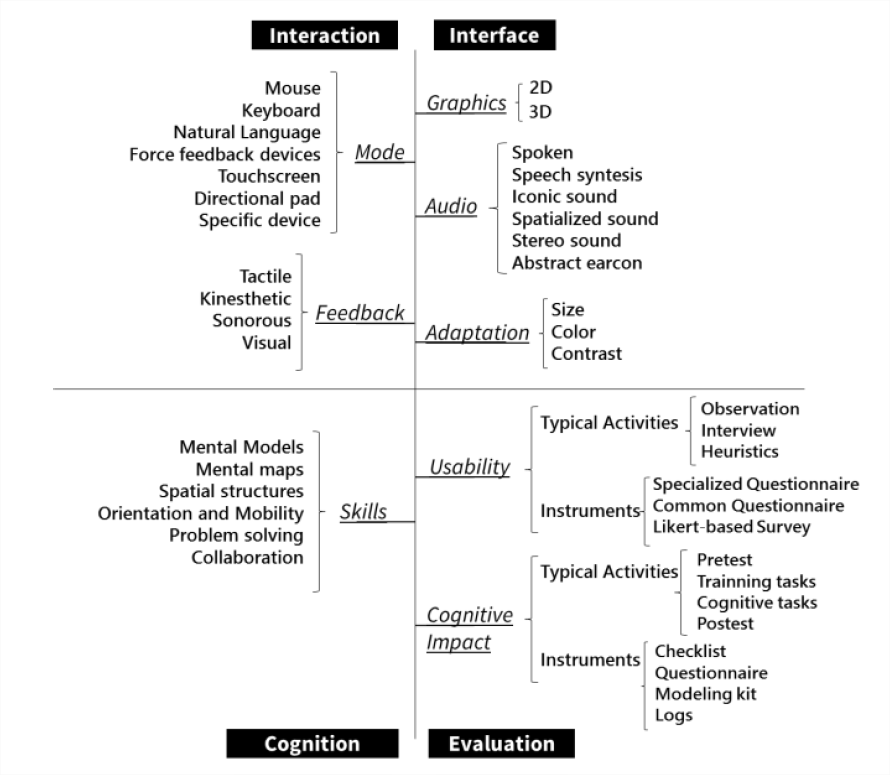
\includegraphics[width=14cm]{figuras/key_features_multimodal_interfaces.png}
		}{
			\Fonte{ \citeonline{Darin2015}.}
		}	
	\end{figure}

For our purpose, we classify only in the interaction, interface and cognition dimensions; and we cover, in the classification, more than video games and virtual environments, since we also found these features present in the technologies selected. These features provide necessary insights for the practical understanding of the issues involved in their design and evaluation \cite{Darin2015}. They are useful in our research for giving a comprehensive overview of technologies and evaluations regarding the multimodal interfaces. The research category still shows more information about the research, as other strategies used to evaluate.

The empirical category provides information specifically about how the empirical method that evaluates the impact of the cognitive impact. These data are more explained in the Results chapter (Section \ref{chap:resultados}).

\section{Grounded Theory}
\label{sec:methodology-gt}

The Grounded Theory, introduced by Barney Glaser and Anselm Strauss, is a method at the beginning used on health studies \cite{Glaser1967}. \citeonline{Glaser1967} contrast theory generated by deduction and a priori assumptions with the theory discovery arising from and grounded in research data, through constant comparison. ``One can argue that every research is somehow "grounded" in data, but using this data from systematic research, together with a set of rigorous research procedures to produce a "grounded theory" is a different approach'' \cite{Motta2016}. The employee of the Grounded Theory method is recent in Empirical Software Engineering. 

The Grounded Theory analysis was performed to enhance and strengthen the findings of the Systematic Literature Review regarding cognitive evaluation concepts used in the context of this search, multimodal interfaces for people who are blind. The data gathered from the literature become the population used in the analysis. We aim analyze in the deepest level of generating theory but as the authors state: knowledge and understanding take many forms \cite{Corbin1998}. The Grounded Theory was supported by the MAXQDA12\footnote{MAXQDA - \url{https://www.maxqda.com/}} tool in the whole process, which is composed of the following steps: planning, data collection, coding and reporting results.

The planning step aims to identify the area of interest and the research question that drives the work. In our case, the area of interest is the Cognitive Impact Evaluation. In the current research, the Grounded Theory suits well some characteristics of cognitive impact experiment extracted from the systematic review as it aids in the interpretation and clarification of the results found. The Grounded Theory methodology comes as a mechanism to understand this data and how they relate to each other considering the application domain and evaluation features.


%%%%Refazer imagem com termos utilizados e sequencia.%%%%

% 	\begin{figure}[h] 
%   	    \captionsetup{width=16cm}%Da mesma largura que a figura
% 		\Caption{\label{fig:grounded_theory__process} Grounded Theory process}
% 		\UFCfig{}{
% 			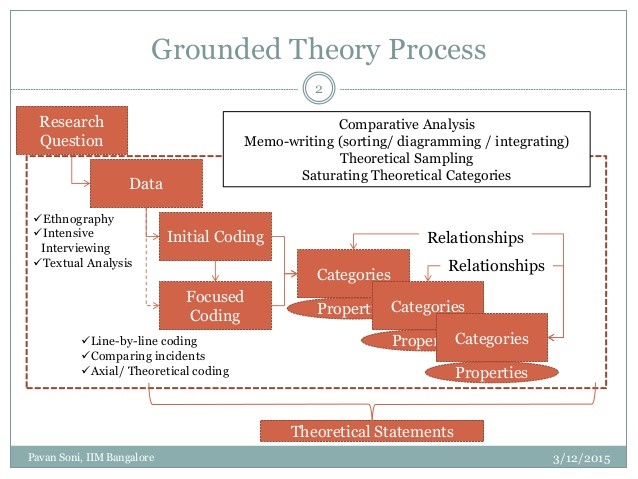
\includegraphics[width=16cm]{figuras/grounded_theory__process.jpg}
% 		}{
% 			\Fonte{ \citeonline{Charmaz2006}.}
% 		}	
% 	\end{figure}

In the data collection step, we prepare an Excel spreadsheet with data from the Systematic Literature Review. We import the data extraction form from each experiment into the MAXQDA. In this way, each experiment is a document in the MAXQDA analysis. All data from experiments are imported as variables (59 variables), that could be used to quantify your qualitative analysis results or to add additional information to pieces of data. These one are already imported as excerpts coded as the empirical categories. 

The data retrieved is organized and modified from the paper to answer the data form. Although, in some experiments, we add some excerpt from the paper to facilitate the coding step on that experiment.

The coding step, the heart of the Grounded Theory, is composed of (i) Open Coding, (ii) Axial Coding, and (iii) Selective Coding. On this step we extracted concepts from raw data and relate them to each other until reaching a core concept \cite{Wuetherick2010}. In our case, we envisioned and related some concepts of experiments of cognitive impact evaluation.

The excerpts coded in this step could be a word, a phrase or a full paragraph when relevant for the concept under observation at the moment. We explore the experiments and open up the data to all potentials and possibilities contained within them \cite{Wuetherick2010}. After considering all possible meanings and examining the context carefully produced 91 codes and 808 tags. Figure \ref{fig:open_coding} shows the 6 top categories of the codes. 

To uncover and develop the concepts one has to keep the mind open and also report thoughts and ideas related to it. The researcher scrutinizes the data in an attempt to understand the essence of what is being expressed in the raw data \cite{Wuetherick2010}. 

 	\begin{figure}[h] 
   	    \captionsetup{width=13cm}%Da mesma largura que a figura
		\Caption{\label{fig:open_coding} Open Coding}
		\UFCfig{}{
			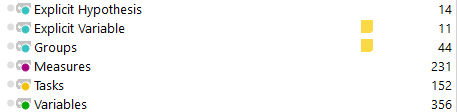
\includegraphics[width=13cm]{figuras/open_coding.png}
		}{
			\Fonte{Produced by the author.}
		}	
	\end{figure}

In the open coding, constant comparative analysis is a regular procedure to execute it. Whenever coming across another excerpt that seemed to talk about the same concept or shared a common attribute, these were grouped together into the same code. 

Axial Coding is stepping to relate concepts to each other \cite{Wuetherick2010}. With this step, the fractions of data from the open coding can be reassembled and organized into the categories and subcategories with their descriptions, properties or dimensions. The Axial Code produced 95 codes and 603 tags. 

The Selective Coding merge all concepts grounded in the process and others captured in the Systematic Literature Review. As a result, we produce maps of concepts and a map to ground the theory of the cognitive impact evaluation in multimodal interfaces for people who are blind or visually impaired. All maps are presented in the chapter Results (Section \ref{chap:resultados}). 

	\chapter{Results}
\label{chap:resultados}

In this chapter, we present the results of the methodology steps. We present both process results as also the data and discussions of each method. Section \ref{sec:results-slr} shows the process results, as for withdrawing paper process. Section \ref{sec:results-theory} explains the Systematic Literature Review process. Section \ref{sec:results-gt} shows the process results. The next sections are focused on the three categories of data acquired and analyzed from both Systematic Literature Review and Grounded Theory. The categories are \textit{(i)} General (Section \ref{sec:results-general}), \textit{(ii)} Research (Section \ref{sec:results-research}), and \textit{(iii)} Empirical (Section \ref{sec:results-empirical}). Finally, Section \ref{sec:results-theory} presents all concepts related to a theory of Cognitive Impact Evaluation for people who are blind.

\section{Systematic Literature Review Results}
\label{sec:results-slr}
We have performed the search, selection and data extraction from the initial systematic literature review process and the snowballing process (forward and backward snowballing). The systematic literature review had four filters for both the initial and the snowballing processes. Appendix \ref{ap:A} details the complete list of selected papers and the spreadsheet\footnote{\url{https://www.dropbox.com/s/dvvn44cymqsqguy/Systematic\%20Review\%20-\%20Mesquita\%20L.\%202018.xlsm?dl=0}} has all data documented. Next, we present the results about the process: papers selected, papers withdrawn and the rates of acceptance.

Figure \ref{fig:filters_in_systematic_review_process} resumes the conducting phase results. The initial search brings us 2173 papers, among them, after the whole process, it remains 23 papers. Further, the snowballing process brings 690 papers (287 from forwarding snowballing and 403 backward snowballing), among them it remains 24 papers (15 from forwarding snowballing and 9 from backward snowballing). Then, at the final process of systematic literature review, we have 47 papers (23 from initial search and 24 from snowballing search). 

 	\begin{figure}[h] 
   	    \captionsetup{width=16cm}%Da mesma largura que a figura
		\Caption{\label{fig:filters_in_systematic_review_process} Filters in the Systematic Review Process}
		\UFCfig{}{
			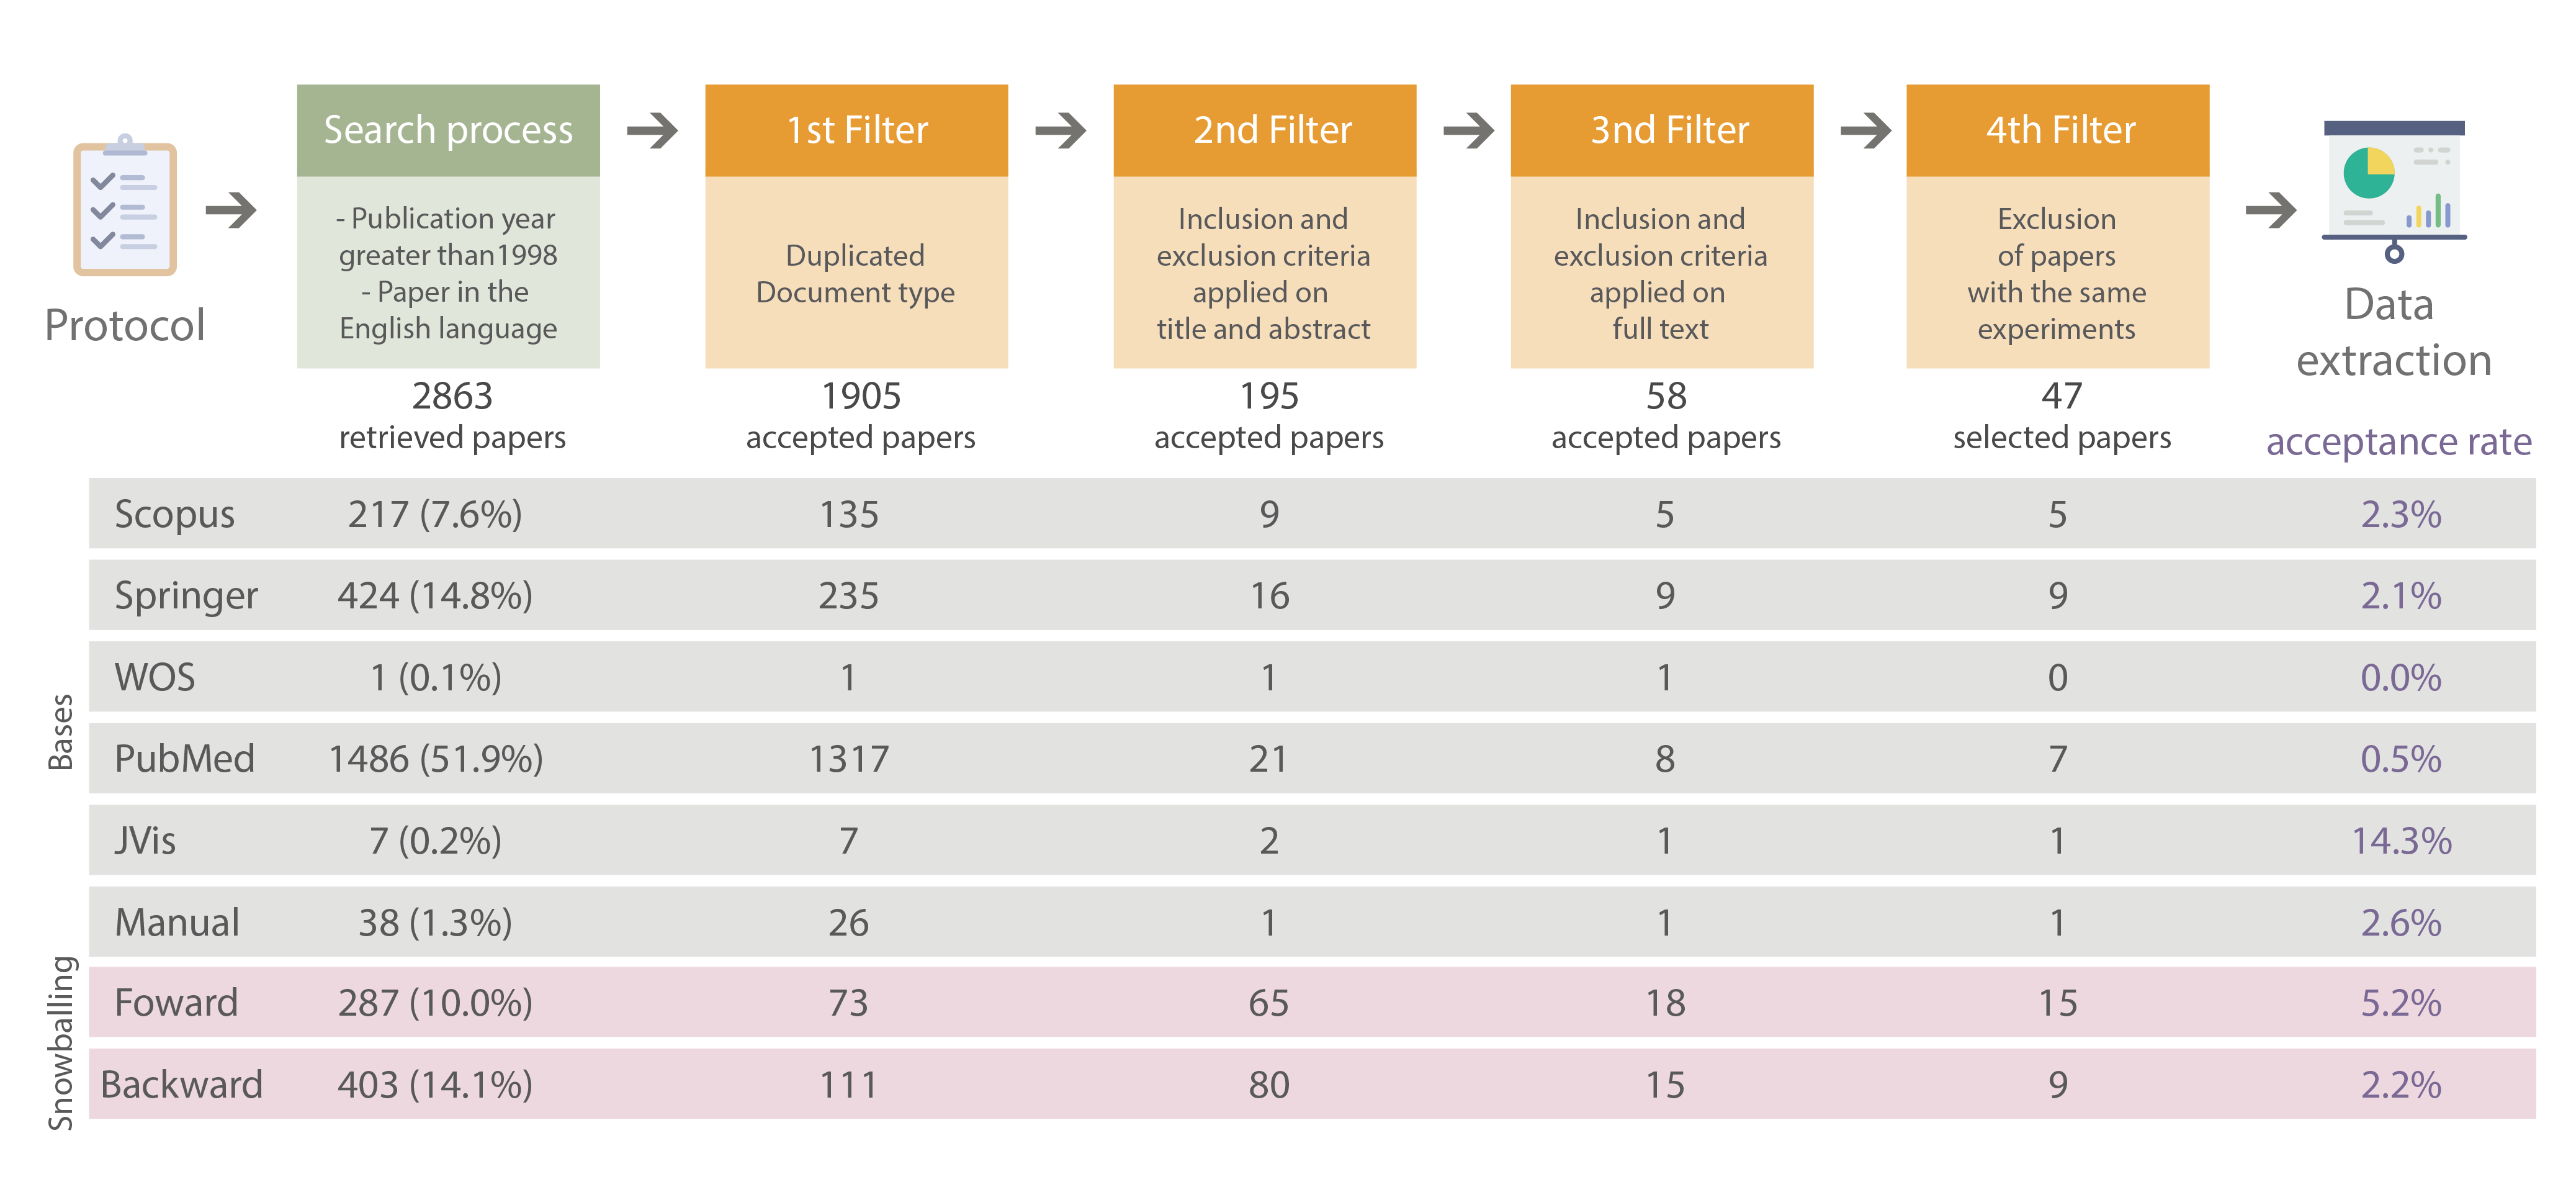
\includegraphics[width=16cm]{figuras/filters_in_systematic_review_process.png}
		}{
			\Fonte{Produced by the author.}
		}	
	\end{figure}

Regarding the acceptance rate (last column of Figure 1), the most important source for this search is the Visual Impairment \& Blindness Journal (\gls{JVis}). The acceptance rate of \gls{JVis} is 14.3\%, which means the number of accepted papers (1 paper) over the number of papers initially retrieved (7 papers). This rate is due to the journal's central theme is the subject sought in this review. Also, we can see that the snowballing process was a good step for the process since it had a large acceptance rate and a large number of papers selected.

Table \ref{tab:Acceptance of papers in_each_filter} shows the acceptance rate of each filter comparing with the last filter, e.g., the acceptance of forwarding snowballing papers in the third filter comparing to the papers selected on the second filter is 27.7\%. In this graph, the snowballing results again stand out. In the second filter, which filters by reading the abstract of the paper, we have an efficient selection with 72.1\% and 89.0\% for backward and forward respectively. These rates reinforce the significance of snowballing in the process.

\begin{table}[h]
	\captionsetup{width=11cm}%Deixe da mesma largura que a tabela
	\Caption{\label{tab:Acceptance of papers in_each_filter} Acceptance of papers in each filter}%
	\IBGEtab{}{%
		\begin{tabular}{m{2cm}m{2cm}m{2cm}m{2cm}m{1cm}}
			\toprule
			 & Total without snowballing & Backward snowballing & Forwarding snowballing & \textbf{Total}\\
			\midrule \midrule
			\textbf{First filter} & 79.2\% & 27.5\% & 25.4\% & \textbf{66.5\%} \\
			\textbf{Second filter} & 2.9\% & 72.1\% & 89.0\% & \textbf{10.2\%} \\
			\textbf{Third filter} & 50.0\% & 18.8\% & 27.7\% & \textbf{29.7\%} \\     
			\textbf{Fourth filter} & 92.0\% & 60.0\% & 83.3\% & \textbf{81.0\%} \\
			\bottomrule
		\end{tabular}%
	}{%
	\Fonte{Produced by the author.}%
%	\Nota{esta é uma nota, que diz que os dados são baseados na	regressão linear.}%
%	\Nota[Anotações]{uma anotação adicional, seguida de várias outras.}%
    }
    \end{table}

To better understand the snowballing process, we track from where each paper came from and how many papers were accepted of each one. Figure \ref{fig:snowballing_acceptance} shows how many papers brings each paper selected in the initial process and how many of them had been selected. We highlight two papers: ``A Virtual Environment for People Who Are Blind – A Usability Study'' \cite{201219} and ``Assessment of Indoor Route-finding Technology for People with Visual Impairment'' \cite{20105}.

 	\begin{figure}[h] 
   	    \captionsetup{width=16cm}%Da mesma largura que a figura
		\Caption{\label{fig:snowballing_acceptance} Snowballing process}
		\UFCfig{}{
			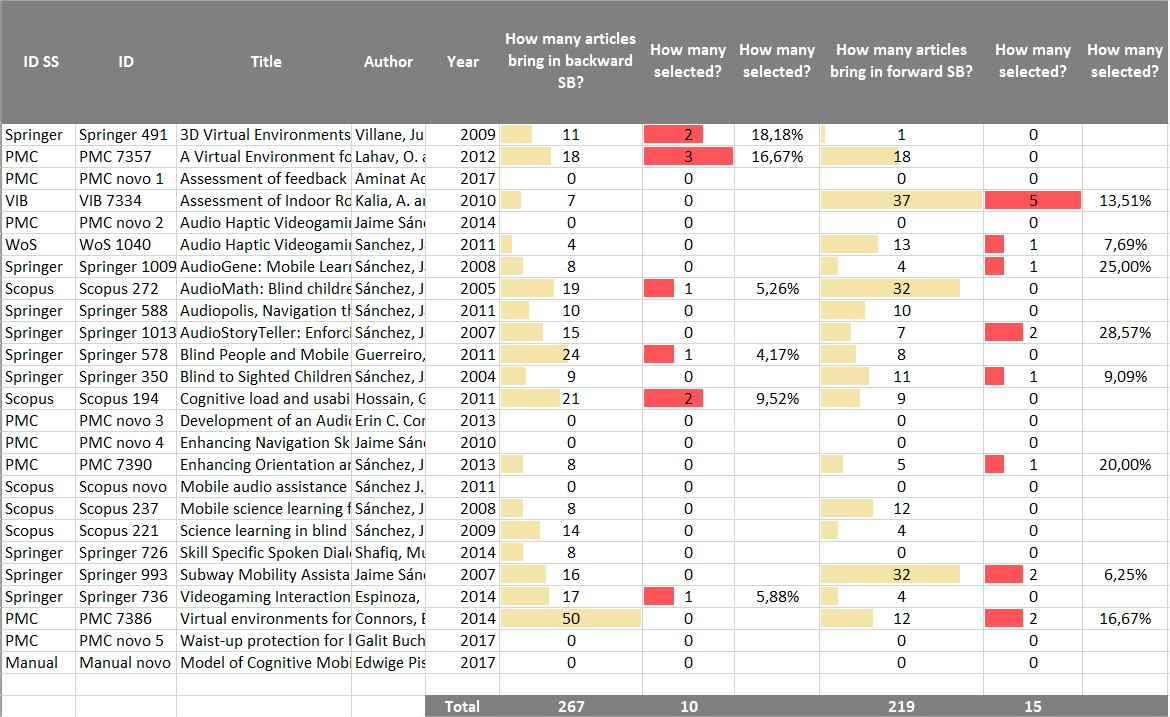
\includegraphics[width=16cm]{figuras/snowballing_acceptance.jpg}
		}{
			\Fonte{Produced by the author.}
		}	
	\end{figure}

\subsection{Withdrawn papers}
\label{subsec:results-slr-withdrawal-papers}

Many papers excluded in the first filter are from the scientific base PubMed Central (\gls{PMC}), this is due to a lot of medical papers focused on disease effectiveness and specific medical statements. Even though the area of this study is computer science, we decided to insert the \gls{PMC} in the bases’ list due to the nature of the subject. To help the exclusion process, we highlighted some keywords not desired in the titles, like ``malaria'' or ``Alzheimer'', which facilitates the exclusion. 

Figure \ref{fig:reasons_for_withdrawn_pappers} shows the reasons for withdrawing papers in the third filter regarding the whole paper and the inclusion criteria. The main reason for withdrawing a paper in the last filter was ``the paper’s evaluation is out the search'' (105 papers excluded), which mainly consider the evaluation focused on the system performance and not on the user cognitive impact assessment. The other reasons are: 
        \begin{enumerate}
            \item The experiment not described in the paper (3 papers);
            \item The paper was not available to download from our online library's catalog of holdings or open access journals (6 papers);
            \item The system is not according to the inclusion criteria (8 papers);
            \item The paper is a Solution Proposal \cite{Petersen2008} focused on, for example, a model or a framework with or without evaluation (4 papers);
            \item The paper is a Philosophical Paper \cite{Petersen2008} (11 papers), e.g., reviews. 
        \end{enumerate}

 	\begin{figure}[h] 
   	    \captionsetup{width=12cm}%Da mesma largura que a figura
		\Caption{\label{fig:reasons_for_withdrawn_pappers} Reasons for paper withdrawn}
		%TODO alterar na figura!
		\UFCfig{}{
			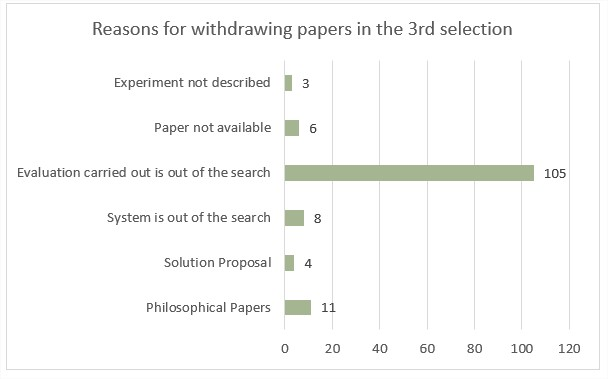
\includegraphics[width=12cm]{figuras/reasons_for_withdrawn_pappers.jpg}
		}{
			\Fonte{Produced by the author.}
		}	
	\end{figure}

% \subsection{Cross Validation}
% \label{subsec:results-slr-cross-validation}

% To reduce the bias, we apply a cross-validation on the third filter selection of the systematic literature review, on which we read the entire papers to select them, regarding the inclusion criteria. We use the selection result to compare with our and to get the accuracy of the filter. We send the quality form to five specialists on HCI themes. We send a list of 20 papers and we expect they validate a sort of 10 papers. 

% At final, two specialists answered, and the accuracy obtained was 59.2\% when comparing the selections of specialists and our selection. Figure \ref{fig:cross_validation} shows the results obtained of each expert. Due to the low rate of answers, we analyze each paper and its reason to withdraw case-by-case. After removing the papers with conflict (one expert accept and the other reject) and the papers with only one answer, we obtained an accuracy of 75.0\%.


%     \begin{figure}[h] 
%   	    \captionsetup{width=12cm}%Da mesma largura que a figura
% 		\Caption{\label{fig:cross_validation_results} Cross-validation Results}
% 		%TODO alterar na figura!
% 		\UFCfig{}{
% 			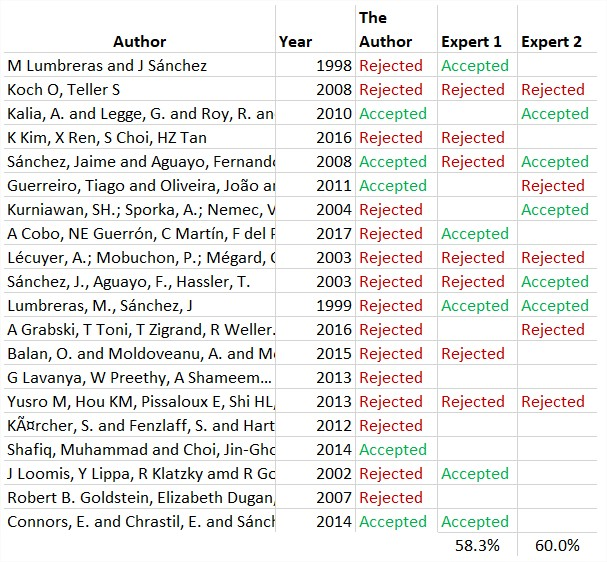
\includegraphics[width=12cm]{figuras/cross_validation_results.jpg}
% 		}{
% 			\Fonte{Produced by the author.}
% 		}	
% 	\end{figure}

\section{Grounded Theory results}
\label{sec:results-gt}
The Grounded Theory analysis was performed to enhance and strengthen the findings of the Systematic Literature Review regarding cognitive evaluation concepts used in the context of this search, multimodal interfaces for people who are blind. The data used came from the systematic literature review process. 

In Grounded Theory, we use the method to analyses in detail four items from Empirical category: Hypothesis, Variables, Measures, and Tasks. The final map produced by the Selective Coding phase (explained in the Section \ref{sec:methodology-gt}) represents the main idea of the cognitive evaluation in the context of this study and connect all elements. This map is the main input to create the Guidelines.

%%%% Comentário do .doc%%%%
%Esse parágrafo foi feito na tentativa de mesclar os resultados e tinha colocado na introdução do capítulo. Porque se dividirmos m resultados da Revi. Sist. e do Ground Theory a categoria de Dados Empíricos será separada. Tanto que já explico na sessão Empirial Data (da Revisão sistemática) quais dados serão analisados por qual método. 

%Se mantiver separado é só desconsiderar este parágrafo.

In the Selective Coding, other elements of cognitive evaluation were mapped in the MAXQDA software to produce the map, as Sample and Ethical Concepts. For this reason, both systematic literature review and grounded theory results are present together in the Empirical section (Section \ref{sec:results-empirical}). The map of central idea is most explored in the Section \ref{sec:results-theory}.

Next, we will explain the data acquired from systematic literature review in the three categories: \textit{(i)} General, \textit{(ii)} Research, and \textit{(iii)} Empirical.

\section{General Results}
\label{sec:results-general}

Despite we consider as the final result of the systematic literature review the papers selected in the fourth filter, in this analysis of general data, we consider the 58 papers selected in the third filter. The type of data used in this category refers to papers within the search criteria. Therefore, it does not need to remove the papers that have cognitive experiments, even if papers have repeated experiments (kind of papers excluded in filter 4).

Regarding the empirical method, almost all papers use an Experiment as an empirical method (21 papers). Only 1 paper present a Case Study as an evaluation, that justifies the choice due to the small number of participants \cite{Sanchez2008}. This information was encountered in the text explicit or it was deducted from the details presented.

Figure \ref{fig:publication_year_of_papers} shows the papers selected regarding the timeline that starts in 2000 and has peaked in 2011 and 2014. These papers, published in the last years, give a comprehensive and valid picture of the existing evidence \cite{Wohlin2000}, considering that both the identification, the analysis, and the interpretation had conducted in a scientifically and rigorous way.

 	\begin{figure}[h] 
   	    \captionsetup{width=16cm}%Da mesma largura que a figura
		\Caption{\label{fig:publication_year_of_papers} Publication year of papers}
		\UFCfig{}{
			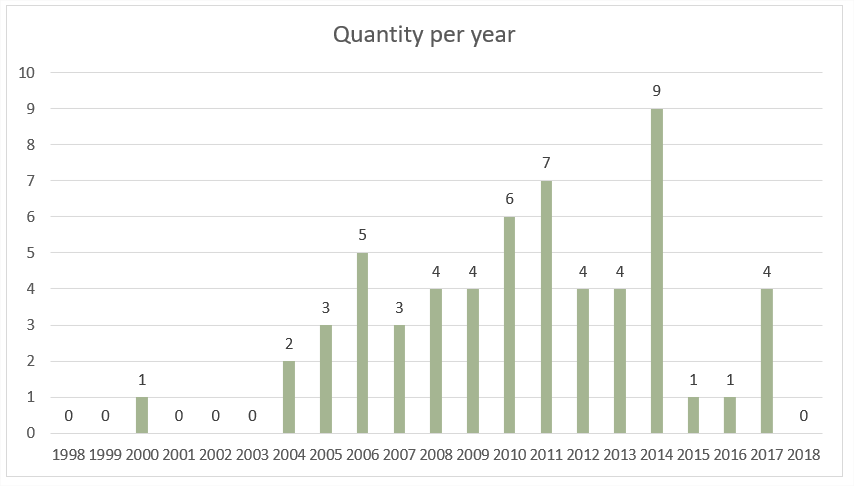
\includegraphics[width=16cm]{figuras/publication_year_of_papers.png}
		}{
			\Fonte{Produced by the author.}
		}	
	\end{figure}
	
\subsection{Qualitative evaluation}
\label{subsec:results-slr-qualitative-evaluation}

Each paper was evaluated according to the 8 questions of the quality form described in Section \ref{subsubsec:conducting-quality} and over again presented in the list below.

\begin{itemize}
    \item \textbf{Q1} Was it possible to extract all data regarding the data the Key features in multimodal interfaces (Classification category from extraction form? (-0.1 pt per missing input; min value: -4.1 pts)
    \item \textbf{Q2} Is there a complete description of how the evaluation has been applied? (1.0 pt per complete input in Empirical category; max value: 8,0 pts)
    \item \textbf{Q3} Are the groups of participants in the experiment randomly assigned? (0.5 pt)
    \item \textbf{Q4} Is the description of the impact evaluation understandable? (0.5 pt)
    \item \textbf{Q5} Does the article present different evaluation types of the proposal? (1 pt)
    \item \textbf{Q6} How many experiments does the paper present? (0.5 pt per experiment, if more than two experiments)
    \item \textbf{Q7} Is the goal of the evaluation cleared defined? (0.5 pt)
    \item \textbf{Q8} Is the hypothesis (null and alternative) explicitly described in the study? (0,5 pt)
\end{itemize}


The results of quality form range from 52\% to 96\% of expected quality, with average of 74\%. The expected quality means the maximum points in each question. We investigated the relationship between the quality score for each paper and both the date when the paper was published. The average quality scores for studies each year is shown in Figure \ref{fig:quality_form_of_papers}.

The quality points were not compared with the impact factor of journals or quality indexes of conferences, as CAPES index quality, and of journals, as h-index. The papers retrieved are from both conferences and journals which already includes the difficulty of comparison. Moreover, some journals and conferences have no index value, or they have different indexes, that also add problems to compare. Then we decided to do not cross this data.

 	\begin{figure}[h] 
   	    \captionsetup{width=16cm}%Da mesma largura que a figura
		\Caption{\label{fig:quality_form_of_papers} Quality form of papers}
		\UFCfig{}{
			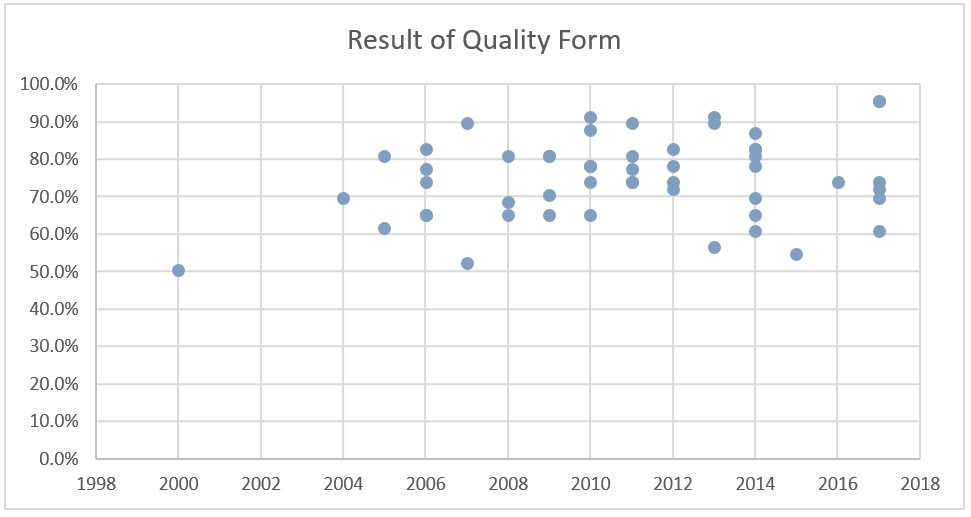
\includegraphics[width=16cm]{figuras/quality_form_of_papers.jpg}
		}{
			\Fonte{Produced by the author.}
		}	
	\end{figure}

\subsection{Publication type}
\label{subsec:results-slr-publication}

Among the papers selected in third filter, 30 are conference papers, 27 are scientific journals, and one is book chapters. The main conferences where the papers selected are published are ACM SIGACCES\footnote{ (\url{https://assets18.sigaccess.org/})} with 6 papers, ICDVRAT \footnote{(\url{https://www.icdvrat.org/})} with 5 papers and UAHCI \footnote{(\url{http://2018.hci.international/uahci})} with 3 papers. The leading journal with three papers retrieved is the International Journal on Disability and Human Development \footnote{(\url{https://www.ncbi.nlm.nih.gov/labs/journals/int-j-disabil-hum-dev/})}.

\subsection{Authors}
\label{subsec:results-slr-authors}

We present an overview of the papers related to cognitive impact evaluation found and how these papers are distributed in the research groups around the world. The papers showed some main authors and institutions that use the cognitive impact evaluation in the context of this research.The authors and research groups distributions contribute to understanding how the cognitive impact evaluation has been applied around the world.

Considering the main authors as those who have more than one paper on the list, Figure \ref{fig:quality_form_of_papers2} shows tag cloud\footnote{Performed in the WordArt tool - \url{https://wordart.com/}} based on the number of papers per authors. Sánchez, J. is the author most present in the list (with 35 papers). Other authors that stand out are Merabet, Lahav, and Sáenz.

 	\begin{figure}[h] 
   	    \captionsetup{width=12cm}%Da mesma largura que a figura
		\Caption{\label{fig:quality_form_of_papers2} Author}
		\UFCfig{}{
			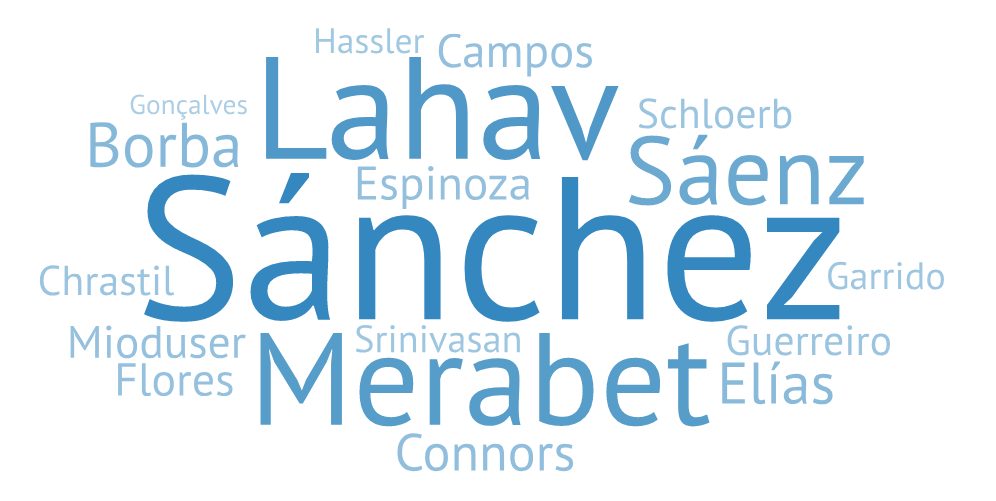
\includegraphics[width=12cm]{figuras/authors.png}
		}{
			\Fonte{Produced by the author.}
		}	
	\end{figure}

Seeking to understand better how and where these authors work, we developed an analysis based on the institutions of origin and found international research relationships between them, explained in the next session.

\textbf{Institutions around the world}

We found the author come from 42 institutions around the world. Figure \ref{fig:mapa} shows the global overview of the papers retrieved. We explore the locations by using the MAXQDA\footnote{\url{https://www.maxqda.com}} software to correlate the groups around the world. As we can see in the figure, the leading research groups in this context are in Chile, USA, and Israel. They are the Department of Computer Science at University of Chile (36 papers, 25,4\% of frequency), Laboratory for Visual Neuroplasticity at Harvard Medical School (8 papers, 5,8\%), School of Education at Tel Aviv University, Israel (7 papers, 4,8\%) and PUCRS in Brazil (4 papers).

\begin{landscape}
 	\begin{figure}[htb] 
   	    \captionsetup{width=25cm}%Da mesma largura que a figura
		\Caption{\label{fig:mapa} The global overview of the papers retrieved}
		\UFCfig{}{
			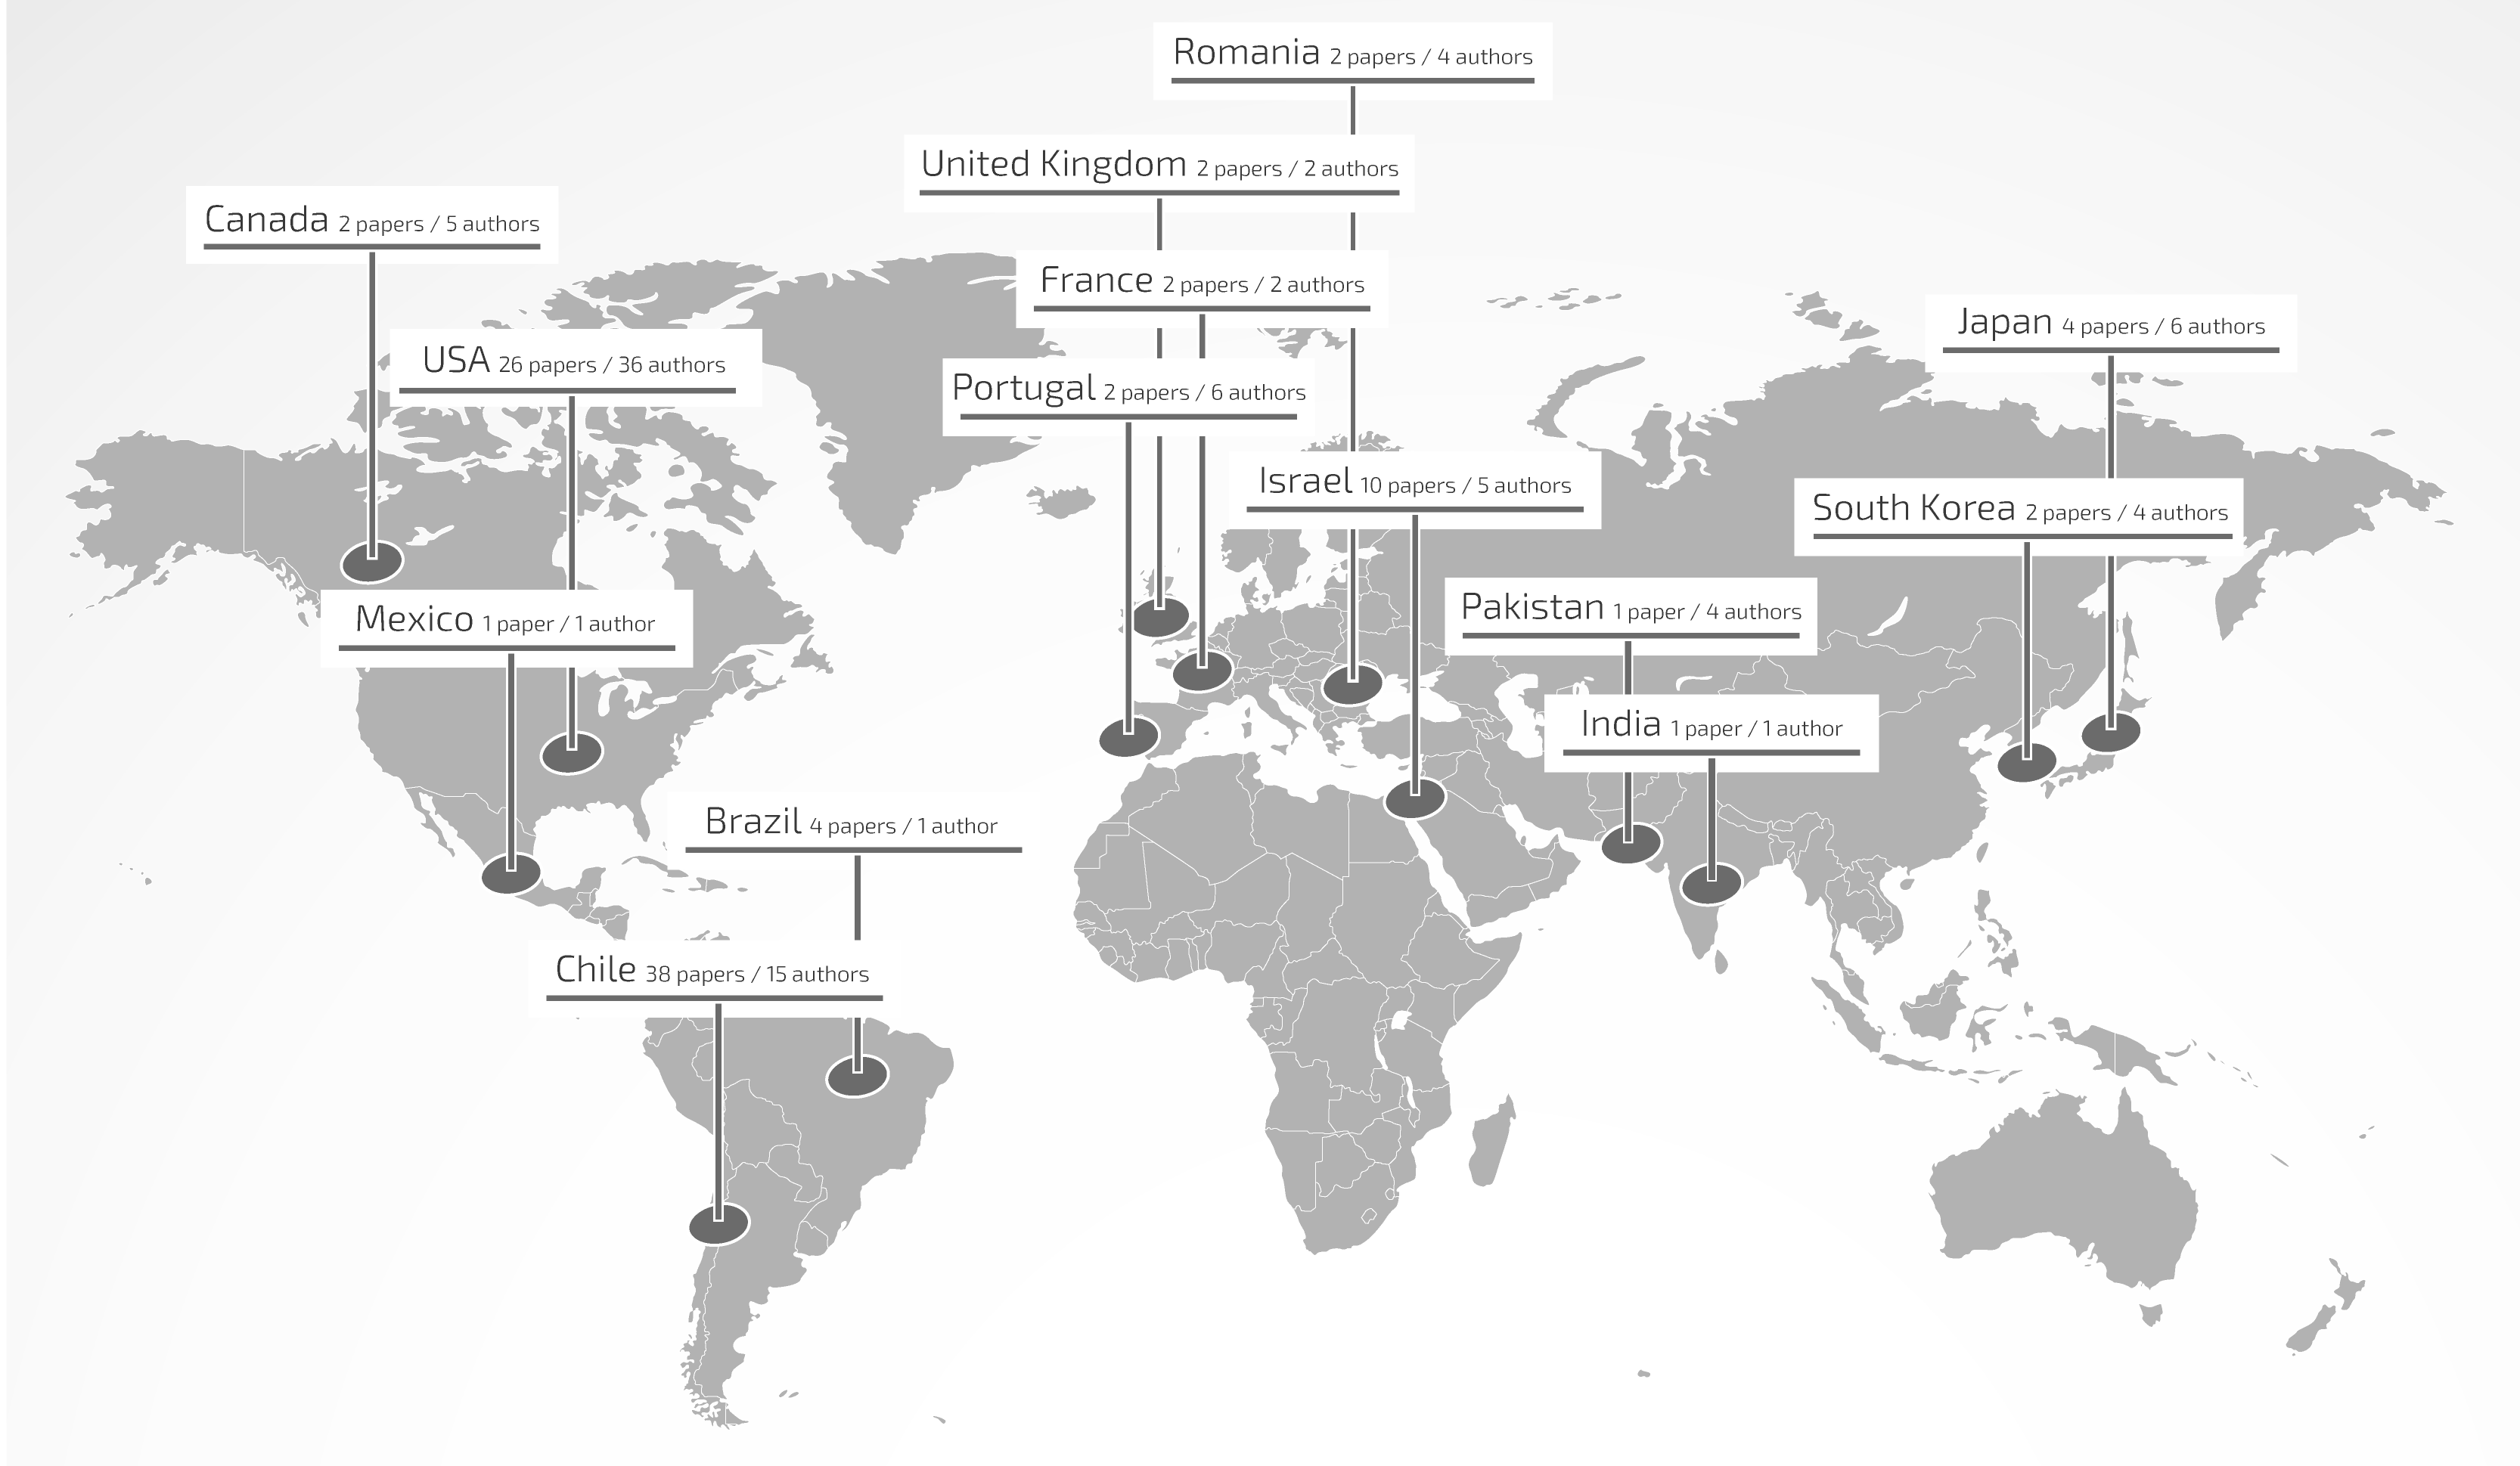
\includegraphics[width=25cm]{figuras/mapa.png}
		}{
			\Fonte{Produced by the author.}
		}	
	\end{figure}
\end{landscape}

The research cooperation between the different institutions is current practice for scientific research, and it is possible to observe in our finds. Table of the Figure \ref{fig:research_between_institutions} shows the cooperation between different institutions, even those are in the same country, as the example of Canada that has 2 institutions working together. In this data, we highlight the large number of institutions and cooperation between them from USA, Chile, and Israel. The USA has great cooperation with Chile and their research institutions. Chile also works with partnerships in Brazilian institutions. Moreover, Israel institutions also stand out by the research with their institutions and with French and American institutions.

\begin{figure}[htb] 
   	    \captionsetup{width=16cm}%Da mesma largura que a figura
		\Caption{\label{fig:research_between_institutions} Research between institutions}
		\UFCfig{}{
			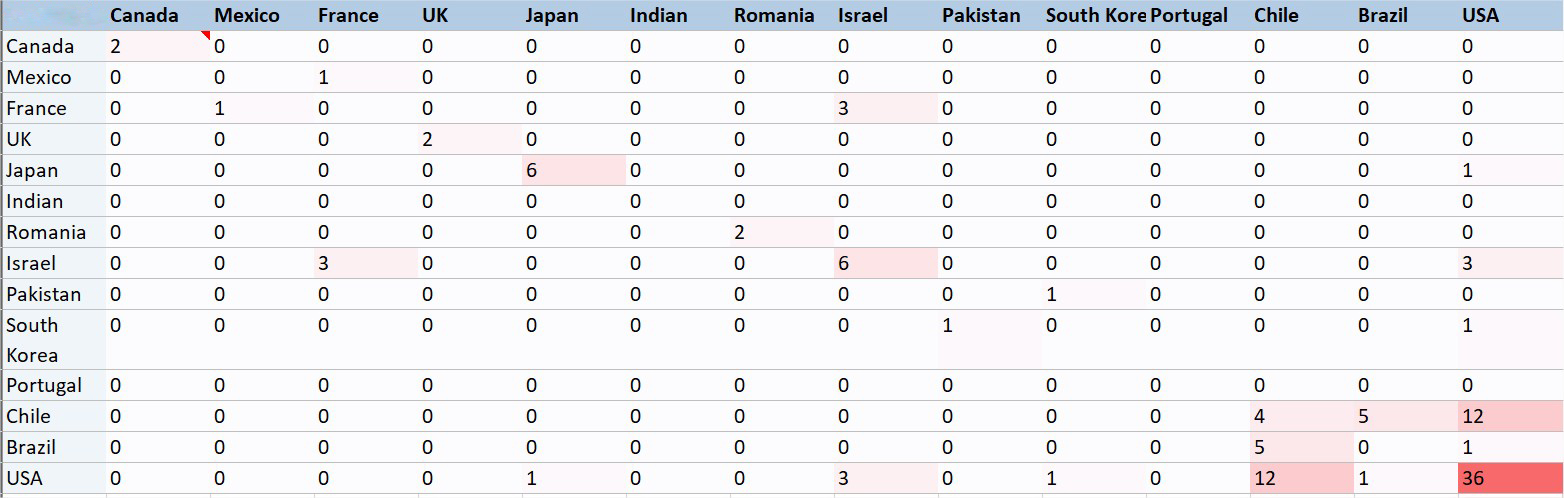
\includegraphics[width=16cm]{figuras/cooperation.jpg}
		}{
			\Fonte{Produced by the author.}
		}	
\end{figure}


%\begin{small}

%\begin{table}[h]
%	\captionsetup{width=16cm}%Deixe da mesma largura que a tabela
%	\Caption{\label{tab:research_between_institutions} Research between institutions}%
%	\IBGEtab{}{%
%		\begin{tabular}{m{1.6cm}m{.55cm}m{.55cm}m{.55cm}m{.55cm}m{.55cm}m{.55cm}m{.55cm}m{.55cm}m{.55cm}m{.55cm}m{.55cm}m{.55cm}m{.55cm}m{.55cm}}
%			\toprule
%			Cooperation System & Cana- da & Me- xico & Fran- ce & UK & Japan & In- dian & Rom- ania & Is- rael & Pakis- tan & South Korea & Portu- gal & Chi- le & Bra- zil & USA\\
			%\cellcolor[HTML]{AA0044} para dar cor a celula basta colar esse codigo antes do valor da celula.
%			\midrule \midrule
%			Canada & 2 & 0 & 0 & 0 & 0 & 0 & 0 & 0 & 0 & 0 & 0 & 0 & 0 & 0 \\
%			Mexico & 0 & 0 & 1 & 0 & 0 & 0 & 0 & 0 & 0 & 0 & 0 & 0 & 0 & 0 \\
%			France & 0 & 1 & 0 & 0 & 0 & 0 & 0 & 3 & 0 & 0 & 0 & 0 & 0 & 0 \\
%			UK & 0 &  0 & 0 & 2 & 0 & 0 & 0 & 0 & 0 & 0 & 0 & 0 & 0 & 0 \\
%			Japan & 0 & 0 & 0 & 0 & 6 & 0 & 0 & 0 & 0 & 0 & 0 & 0 & 0 & 1 \\
%			Indian & 0 & 0 & 0 & 0 & 0 & 0 & 0 & 0 & 0 & 0 & 0 & 0 & 0 & 0 \\
%			Romania & 0 & 0 & 0 & 0 & 0 & 0 & 2 & 0 & 0 & 0 & 0 & 0 & 0 & 0 \\
%			Israel & 0 & 0 & 3 & 0 & 0 & 0 & 0 & 6 & 0 & 0 & 0 & 0 & 0 & 3 \\
%			Pakistan & 0 & 0 & 0 & 0 & 0 & 0 & 0 & 0 & 0 & 1 & 0 & 0 & 0 & 0 \\
%			South Korea & 0 & 0 & 0 & 0 & 0 & 0 & 0 & 0 & 1 & 0 & 0 & 0 & 0 & 1 \\ 
%			Portugal & 0 & 0 & 0 & 0 & 0 & 0 & 0 & 0 & 0 & 0 & 0 & 0 & 0 & 0 \\
%			Chile & 0 & 0 & 0 & 0 & 0 & 0 & 0 & 0 & 0 & 0 & 0 & 4 & 5 & 12 \\
%			Brazil & 0 & 0 & 0 & 0 & 0 & 0 & 0 & 0 & 0 & 0 & 0 & 5 & 0 & 1 \\
%			USA & 0 & 0 & 0 & 0 & 1 & 0 & 0 & 3 & 0 & 1 & 0 & 12 & 1 & 36 \\
%			\bottomrule
%		\end{tabular}%
%	}{%
%	\Fonte{Autor.}%
%	\Nota{esta é uma nota, que diz que os dados são baseados na	regressão linear.}%
%	\Nota[Anotações]{uma anotação adicional, seguida de várias outras.}%
 %   }
 %   \end{table}   
%\end{small}

\subsection{Tools evaluated}
\label{subsec:results-tools}

Finally, in the general data acquired, we search to understand which kind of technology the studies present and evaluate. We search a broader view of tools, which means the tool or application should not have to be specific for people who are blind or visually impaired, but it needs to have into the technology search criteria specified in the Section \ref{subsec:methodology-conducting} and must have a cognitive impact evaluation. A non-standard example of applications found is a study that assesses the cognitive impact of an ATM machine by people who are blind. 

Some papers develop the cognitive evaluation with the same tool, thus, we detect 45 tools evaluated among papers selected. Appendix \ref{ap:A} list all tools detailed. The tools and applications were classified according to the type of activity performed into 8 categories: 
        \begin{enumerate}
            \item School learning: applications that improve school subjects such as mathematics and biology;
            \item Game: applications with gamification elements that develop cognitive characteristics;
            \item Maps: applications that works with indoor and outdoor maps whether virtual or real to develop cognitive navigation, mobility or orientation processes;
            \item Others, as objects structure learning, input text on a telephone keypad, mobile device and ATM machine.
        \end{enumerate}

Figure \ref{fig:technology_type} shows the results of classification. The applications that works with maps, mobility, orientation and navigation are the most common.

 	\begin{figure}[h] 
   	    \captionsetup{width=12cm}%Da mesma largura que a figura
		\Caption{\label{fig:technology_type} Technology type}
		\UFCfig{}{
			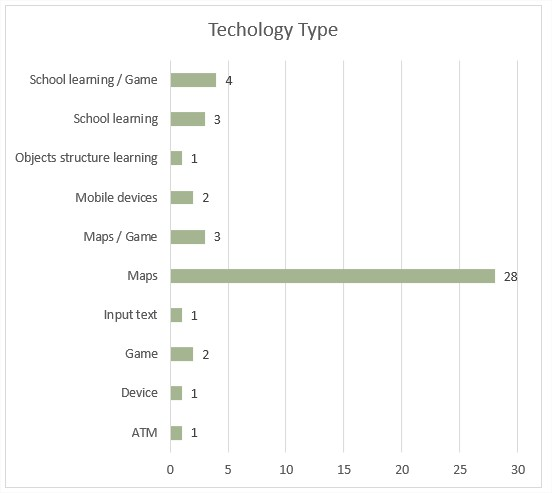
\includegraphics[width=12cm]{figuras/technology_type.jpg}
		}{
			\Fonte{Produced by the author.}
		}	
	\end{figure}

\section{Research results}
\label{sec:results-research}
This category aims to understand the focus of each paper regarding the research done. First, we present others strategies of the technology evaluation encountered in the selected papers. 

\subsection{Other Strategies of the evaluation applied}
\label{subsec:results-other-strategies}

Many papers apply another approach to evaluate other criteria not covered in our study, as shown in Figure \ref{fig:other_strategies}. Usability evaluation is the most used assessment besides impact evaluation. This kind of assessment is mainly used to obtain information about the user's acceptance of the software, and the match between his or her mental model and the representation included in the software \cite{Sanchez2009a}. Others are evaluation based on HCI heuristics \cite{Shafiq2014}, iconic evaluation \cite{Sanchez2011}, recognition of patterns, obstacle awareness goal and homing and obstacle avoidance \cite{Pissaloux2017TowardsDevices}.

 	\begin{figure}[h] 
   	    \captionsetup{width=12cm}%Da mesma largura que a figura
		\Caption{\label{fig:other_strategies} Quantity of other evaluation strategies used}
		\UFCfig{}{
			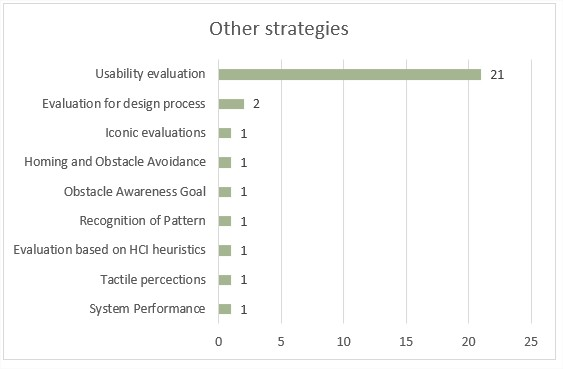
\includegraphics[width=12cm]{figuras/other_strategies.jpg}
		}{
			\Fonte{Produced by the author.}
		}	
	\end{figure}

\subsection{Classification}
\label{subsec:results-classification}

The classification of the key features in multimodal interfaces for the cognition of people who are blind proposed by \citeonline{Darin2015} is adapted to classify the papers, already presented in Figure \ref{fig:Key_features _in_multimodal_interfaces_(evaluation)}. This classification is divided into 4-dimension: Interface, Interaction, Cognition, and Evaluation; and it is applied to video games and virtual environments. These features provide necessary insights for the practical understanding of the issues involved in their design and evaluation \citeonline{Darin2015}. These features are useful in our research for giving a comprehensive overview of technologies and evaluations regarding the multimodal interfaces.

We cover, in the classification, more than video games and virtual environments since we also found these features present in the technologies selected. We did not divide the features of the evaluation domain into cognitive and usability evaluation. Instead, we focus on typical activities and instruments, which in our perception can be applied to the impact evaluations that were found. Then, the result of this classification is shown in Figure \ref{fig:key_features_evaluation}.

 %	\begin{figure}[h] 
  % 	    \captionsetup{width=16cm}%Da mesma largura que a figura
%		\Caption{\label{fig:key_features_multimodal_interfaces_results} Key features in multimodal interfaces}
%		\UFCfig{}{
%			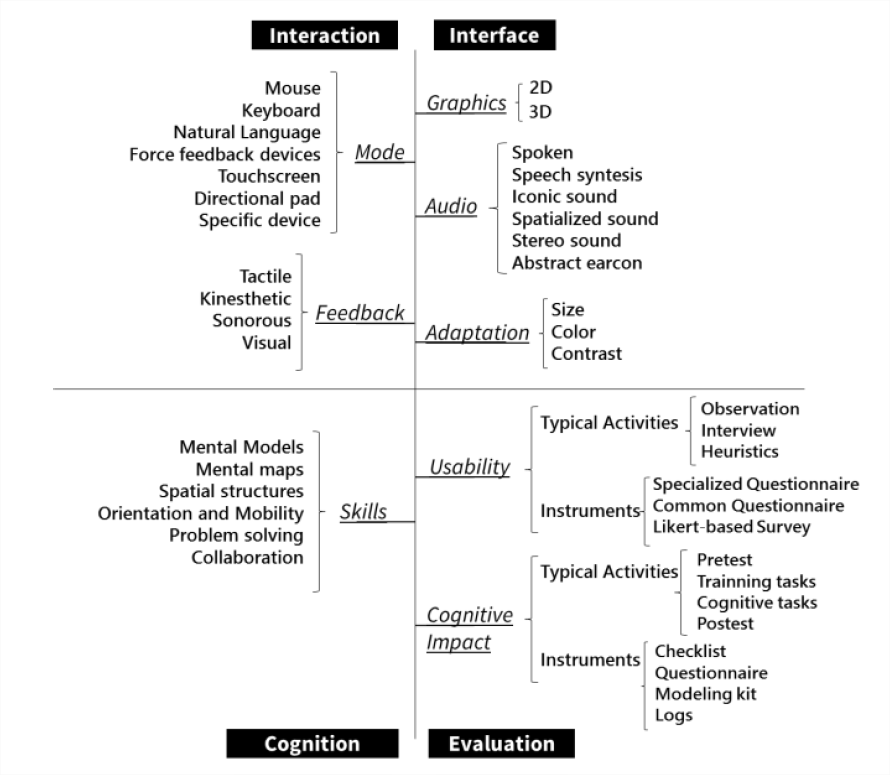
\includegraphics[width=16cm]{figuras/key_features_multimodal_interfaces.png}
%		}{
%			\Fonte{\citeonline{Darin2015}.}
%		}	
%	\end{figure}
	
 	\begin{figure}[h] 
   	    \captionsetup{width=12cm}%Da mesma largura que a figura
		\Caption{\label{fig:key_features_evaluation} Key features in multimodal interfaces (Evaluation)}
		\UFCfig{}{
			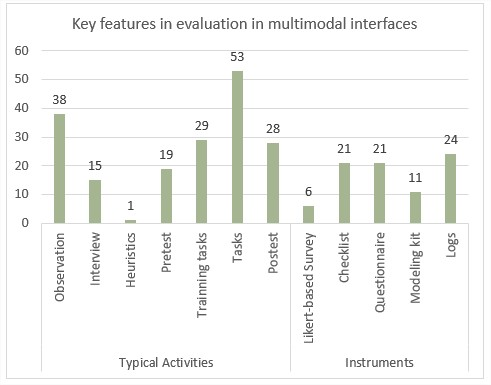
\includegraphics[width=12cm]{figuras/key_features_evaluation.jpg}
		}{
			\Fonte{Produced by the author.}
		}	
	\end{figure}


As we can see, the Keyboard is the main mode to interact with technologies analyzed. It is an instrument of interaction already common as input device \cite{Sanchez2004}. The keyboard does not generate more complexity and expenses, like the Novint Falcon device, that is used in \cite{Sanchez2014a}. The Novint Falcon is one of the Force Feedback Device that promotes a Tactile and Kinesthetic Feedback. Mouse and Natural language are less used. The mouse is replaced by buttons or other specific devices for a better interaction, as shown in \cite{Shafiq2014}. The most common Feedback is the Sonorous and the main Audio Interface used is the Iconic Sound, which are sounds associated with each available object and action in the environment \cite{Sanchez2014a}.

These characteristics are important to understand which kind of interfaces are assessed and how the impact is evaluated on them. The Evaluation dimension will be discussed in more depth in the following sections.

\section{Empirical data results}
\label{sec:results-empirical}

The Empirical category aims to answer the research question of the systematic literature review in detail. The data retrieved ground the comprehension of the main research question. Thus, we search the main aspects concerning the empirical method applied. Note, in this category, we analyze the 47 papers selected on the fourth filter that brings 52 experiments process since five papers have two different experiments. In addition to the Systematic Literature Review (SLR) method, we use the Grounded Theory method to analyze the empirical data. With this combination of methods, we construct a concept based on cognitive assessment data. Figure \ref{fig:Key_features _in_multimodal_interfaces_(evaluation)} shows the data were chosen to be retrieved and which method had been primarily used.

 	\begin{figure}[h] 
   	    \captionsetup{width=12cm}%Da mesma largura que a figura
		\Caption{\label{fig:Key_features _in_multimodal_interfaces_(evaluation)} Empirical data extracted from experiments}
		\UFCfig{}{
			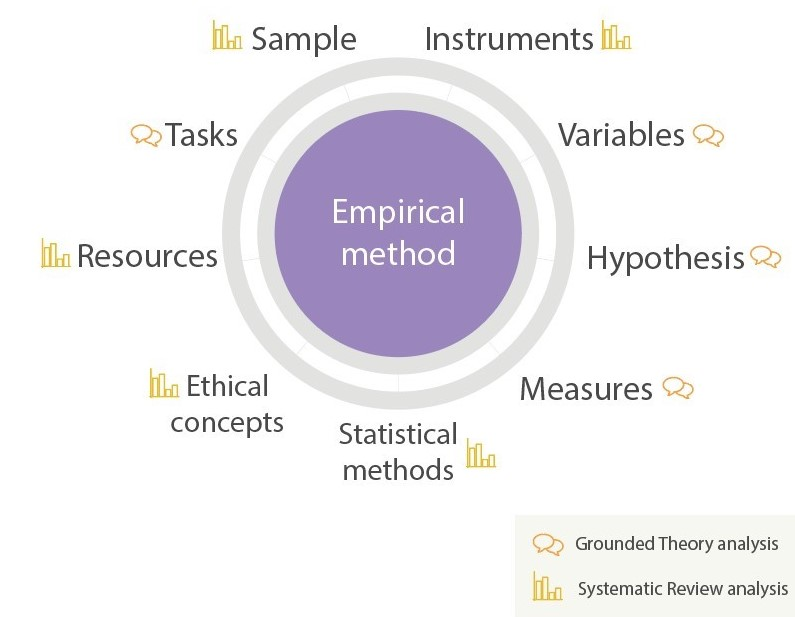
\includegraphics[width=12cm]{figuras/Key_features_in_multimodal_interfaces_(evaluation).jpg}
		}{
			\Fonte{Produced by the author.}
		}	
	\end{figure}

\subsection{Sample}
\label{subsec:results-sample}

In the sample data analysis, we look for the sampling strategy and the samples description, including the number of participants (per condition) and the kind of participants (e.g., computer science students). Figure \ref{fig:sample_information} shows the sample information retrieved from each experiment. This information is one of the main specificities of the type of experiment sought here, that is, of the cognitive evaluation of multimodal interfaces for people who are blind.
%\begin{landscape}
	\begin{figure}[h] 
       \captionsetup{width=15cm}%Da mesma largura que a figura
	\Caption{\label{fig:sample_information} Sample information}
	\UFCfig{}{
		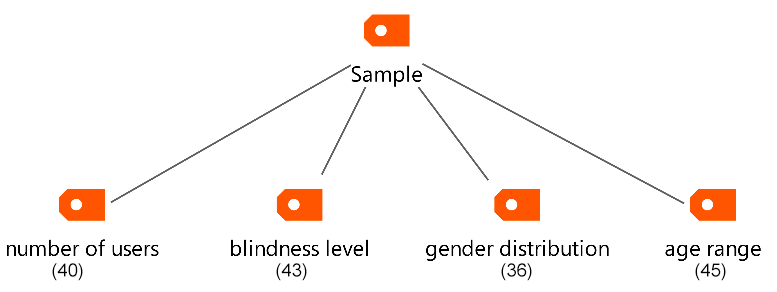
\includegraphics[width=15cm]{figuras/sample_information.png}
	}{
		\Fonte{Produced by the author.}
	}	
	\end{figure}
%\end{landscape}


\textbf{Number of users}

From the number of users to the onset age of blindness, there are many sample combinations in the selected experiments. The sample choice includes previous experience required to do the task and others characteristic controlled in the experiment, like disabilities, the onset of blindness, the etiology of a visual impairment or the presence of another disability. The quantity of users varies as shown in Figure \ref{fig:number_of_users}. Most of the experiments (22) are applied to 6 to 10 users. One experiment does not inform the number of users. One experiment \cite{Hossain2011} expresses the small number of the sample (4 blinds participants) as a limitation/implication of the research. Moreover, the paper talks about the limited access to people who are blind, and those who use a smartphone are even more difficult.

There is no guideline about the number of users on an experiment sample in the context of this research. The tradeoff between limitations and quality of the research should define the number of users. The planning phase must propose a plausible solution with the group of participants that are sought to the experiment have a reasoned result, preferably based on statistical data.

	\begin{figure}[h] 

   	    \captionsetup{width=12cm}%Da mesma largura que a figura
		\Caption{\label{fig:number_of_users} Number of users}
		\UFCfig{}{
			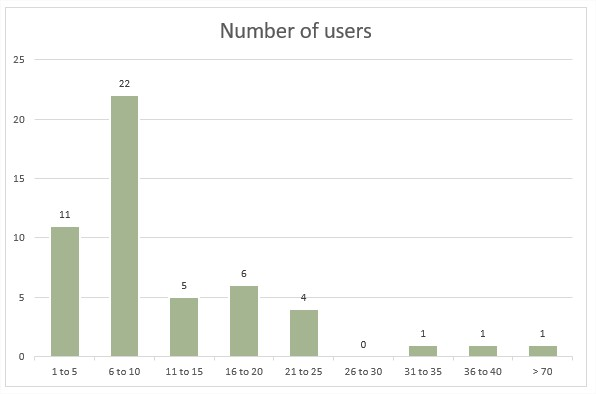
\includegraphics[width=12cm]{figuras/number_of_users.jpg}
		}{
			\Fonte{Produced by the author.}
		}	
	\end{figure}

\textbf{Gender distribution}

The gender distribution in samples is equilibrated in most cases. Figure \ref{fig:gender} shows the gender distribution on each experiment that describes how many women and men are participants (36 papers). The mean of gender proportion, among all samples, is 47\% for women and 53\% for men.

	\begin{figure}[h] 

   	    \captionsetup{width=16cm}%Da mesma largura que a figura
		\Caption{\label{fig:gender} Gender distribution}
		\UFCfig{}{
			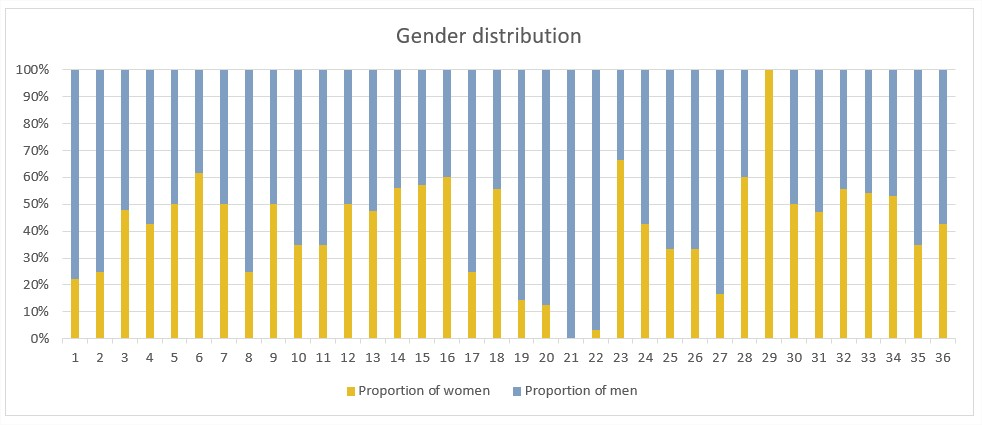
\includegraphics[width=16cm]{figuras/gender.jpg}
		}{
			\Fonte{Produced by the author.}
		}	
	\end{figure}

\textbf{Age range}

The rage of age varies a lot among the experiments. Figure 1\ref{fig:age_range} shows for each experiment the age range (green bar) and the mean (yellow line). To find a pattern, we adopted age groups based on indications of the Brazilian Child and Adolescent Statute (ECA) \cite{CasaCivil1990EstatutoAdolescente} and the Brazilian Statute of the Elderly \cite{CasaCivil2003EstatutoIdoso}, which defines 4groups: child (under age12), adolescent (between age 12 and under 21) , adult (between age 21 and 59) and elderly (over 60 years old). Figure \ref{fig:age_range_2} shows the distribution among age groups. The most of experiments (20 experiments) are applied in adults. 7 experiments do not inform the age of participants.

	\begin{figure}[h] 

   	    \captionsetup{width=16cm}%Da mesma largura que a figura
		\Caption{\label{fig:age_range} Age range of users}
		\UFCfig{}{
			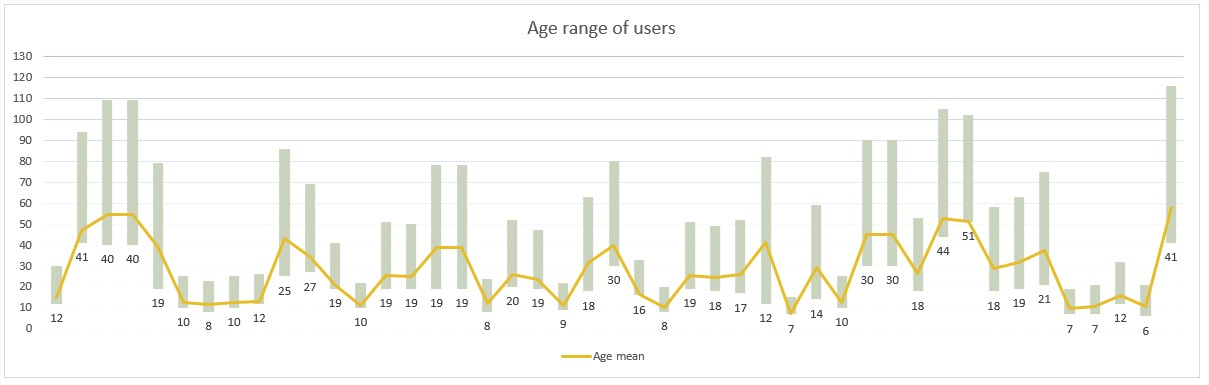
\includegraphics[width=16cm]{figuras/age_range.jpg}
		}{
			\Fonte{Produced by the author.}
		}	
	\end{figure}

	\begin{figure}[h] 

   	    \captionsetup{width=12cm}%Da mesma largura que a figura
		\Caption{\label{fig:age_range_2} Age distribution by groups}
		\UFCfig{}{
			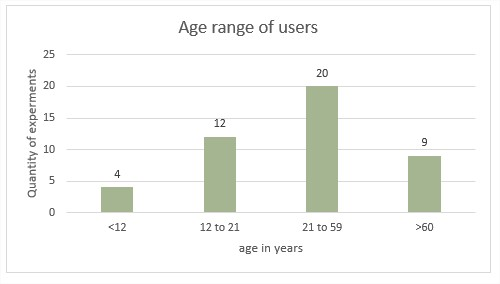
\includegraphics[width=12cm]{figuras/age_range_2.jpg}
		}{
			\Fonte{Produced by the author.}
		}	
	\end{figure}

\textbf{Blindness level}

%%%%Comentário do .doc%%%%%%%%%
%%%Explorar mais a importância desta informação, da seleção desse número e citar os pontos fora da curva: 
%18 artigos só tem pessoas cegas 
%1 artigo só tem pessoas videntes (explicar pq esse entrou) 
%4 artigos utilizam blindfolded --- citar artigo que explica pq não é bom usar blindfolded
%falar ainda de outras informações sobre o nível de cegueira, como onset, origem, tempo, se nasceu ou se se tornou ao longo da vida, se possui outras deficiências... 
%além disso informar, se possível, o nível de cegueira na escala apresentada na fundamentação teórica
%%%

The distribution between the blindness level is varied. There are experiments where the sample is all formed by people who are blind \cite{Lahav2012,Sanchez2005c}, and there are samples formed only by people who are blindfolded, as the experiments in \cite{Pissaloux2017TowardsDevices}. Table \ref{tab:blindproportion} shows the blindness level distribution between the samples. Although it is essential information in the context of the experiments studied here, 9 experiments do not inform the proportions of blind, low vision, sighted and blindfolded. 
\begin{comment}

%%% Tabela excluida e comentada %%%
\begin{table}[h]
	\captionsetup{width=14cm}%Deixe da mesma largura que a tabela
	\Caption{\label{tab:blindproportion} Kind of Instruments}%
	\IBGEtab{}{%
		\begin{tabular}{m{3cm}m{3.5cm}m{3cm}m{3cm}}
			\toprule
		    Proportion of blind & Proportion of low vision & Proportion of Sighted & Proportion of blindfolded \\
			\midrule \midrule
			100\% & 0\% & 0\% & 0\% \\
			100\% & 0\% & 0\% & 0\% \\
			100\% & 0\% & 0\% & 0\% \\
			100\% & 0\% & 0\% & 0\% \\
			100\% & 0\% & 0\% & 0\% \\
			100\% & 0\% & 0\% & 0\% \\
			100\% & 0\% & 0\% & 0\% \\
			100\% & 0\% & 0\% & 0\% \\
			100\% & 0\% & 0\% & 0\% \\
			100\% & 0\% & 0\% & 0\% \\
			100\% & 0\% & 0\% & 0\% \\
			100\% & 0\% & 0\% & 0\% \\
			100\% & 0\% & 0\% & 0\% \\
			100\% & 0\% & 0\% & 0\% \\
			100\% & 0\% & 0\% & 0\% \\
			100\% & 0\% & 0\% & 0\% \\
			100\% & 0\% & 0\% & 0\% \\
			100\% & 0\% & 0\% & 0\% \\
			93\% & 7\% & 0\% & 0\% \\
			80\% & 20\% & 0\% & 0\% \\
			80\% & 20\% & 0\% & 0\% \\
			75\% & 25\% & 0\% & 0\% \\
			75\% & 25\% & 0\% & 0\% \\
			67\% & 33\% & 0\% & 0\% \\
			56\% & 44\% & 0\% & 0\% \\
			53\% & 47\% & 0\% & 0\% \\
			52\% & 48\% & 0\% & 0\% \\
			51\% & 3\% & 44\% & 0\% \\
			50\% & 50\% & 0\% & 0\% \\
			50\% & 0\% & 0\% & 50\% \\
			50\% & 0\% & 0\% & 50\% \\
			44\% & 56\% & 0\% & 0\% \\
			43\% & 57\% & 0\% & 0\% \\
			35\% & 65\% & 0\% & 0\% \\
			33\% & 67\% & 0\% & 0\% \\
			29\% & 71\% & 0\% & 0\% \\
			25\% & 75\% & 0\% & 0\% \\
			25\% & 38\% & 38\% & 0\% \\
			22\% & 0\% & 0\% & 78\% \\
			22\% & 0\% & 0\% & 78\% \\
			20\% & 80\% & 0\% & 0\% \\
			0\% & 100\% & 0\% & 0\% \\
			0\% & 0\% & 100\% & 0\% \\
			\bottomrule 
		\end{tabular}%
	}{%
	\Fonte{Produced by the author.}%
%	\Nota{esta é uma nota, que diz que os dados são baseados na	regressão linear.}%
%	\Nota[Anotações]{uma anotação adicional, seguida de várias outras.}%
    }
    \end{table}
\end{comment}


%\begin{comment}
	\begin{figure}[h] 

   	    \captionsetup{width=16cm}%Da mesma largura que a figura
		\Caption{\label{tab:Kind_of_Instruments} Proportion of blindness level}
		\UFCfig{}{
			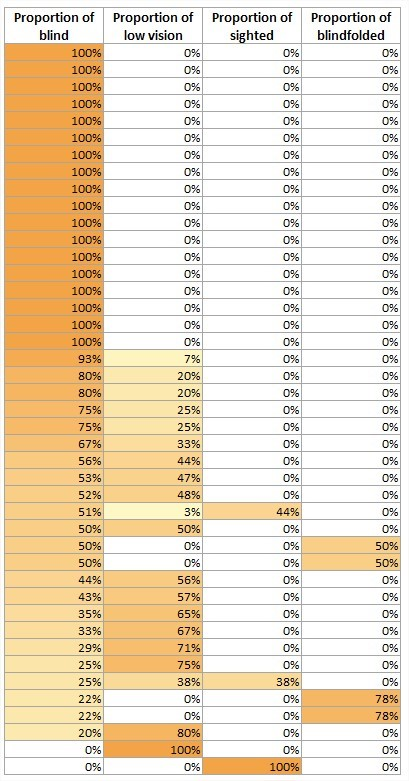
\includegraphics[width=10cm]{figuras/kind_of_instruments.jpg}
		}{
			\Fonte{Produced by the author.}
		}	
	\end{figure}
%\end{comment}

\subsection{Instruments}
\label{subsec:results-instruments}

The instruments used in the evaluation has the objective to identify some user ability controlled on the Experiment (as an independent variable), e.g., the mathematics knowledge test in \citeonline{Sanchez2005,Sanchez2005c} or is used to guide the evaluation process, e.g., observation guideline to assess O\&M skills in \citeonline{Sanchez2011}. 37 experiments described the instruments used. Among the instruments used, there are 5 Likert-based surveys, 20 checklists (which include guidelines and specific tests), 15 questionnaires (which include surveys), 8 modeling kits (which are manual instruments, as pen and papers or bricks), and 9 logs (which include, in addition to the system log, the video and audio logs). None instrument has been used in more than one study experiment from our list. We speculate this is due to the distinct natures of skills evaluated. Figure \ref{fig:kind} shows the ethical concepts retrieved.

	\begin{figure}[h] 

   	    \captionsetup{width=12cm}%Da mesma largura que a figura
		\Caption{\label{fig:kind} Type of Instruments}
		\UFCfig{}{
			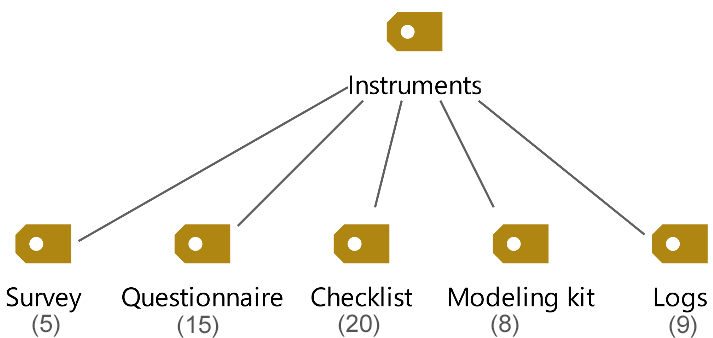
\includegraphics[width=12cm]{figuras/kind.png}
		}{
			\Fonte{Produced by the author.}
		}	
	\end{figure}

\subsection{Statistical Methods}
\label{subsec:results-statistical-methods}

Figure \ref{fig:statistical_methods} shows the statistical methods used in the experiment data analysis. We do not take account of the common statistical methods, like averages and gain percent. In 3 experiments, the statistical method was not described or explicit in the text, neither in the references. T-test, which uses statistical concepts to reject or not a null hypothesis, is the most used, followed by ANOVA and Person’s Correlation, that is used to analyze the variation between groups. ANOVA procedure was applied in one, two and three-way. 

	\begin{figure}[h] 

   	    \captionsetup{width=16cm}%Da mesma largura que a figura
		\Caption{\label{fig:statistical_methods} Statistical methods}
		\UFCfig{}{
			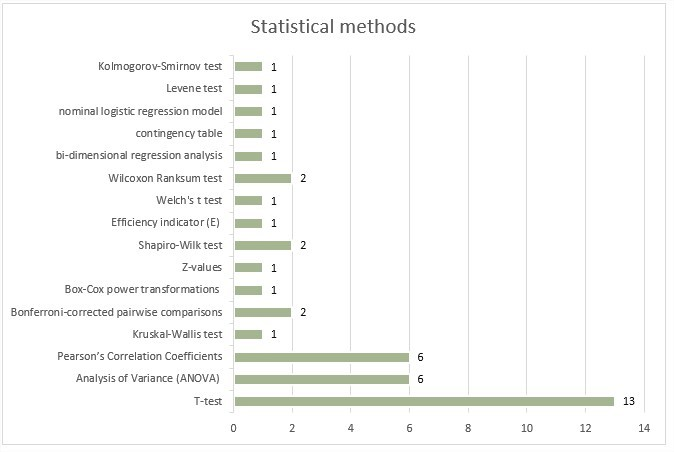
\includegraphics[width=16cm]{figuras/statistical_methods.jpg}
		}{
			\Fonte{Produced by the author.}
		}	
	\end{figure}

The statistical method used depends on the research goal and the data acquired of the experiment. Thus, we prefer not to present the methods according to the type of analysis, such as hypothesis analysis or correlation between variables. Instead, we focused on if the experiment data analysis has any statistical method applied. Our objective is not to discuss how to apply the best method, but to analyze the evidence based on statistical confirmations. However Figure \ref{fig:statistical_type} presents the two types of use to the statistical methods.

	\begin{figure}[h] 

   	    \captionsetup{width=12cm}%Da mesma largura que a figura
		\Caption{\label{fig:statistical_type} Statistical type}
		\UFCfig{}{
			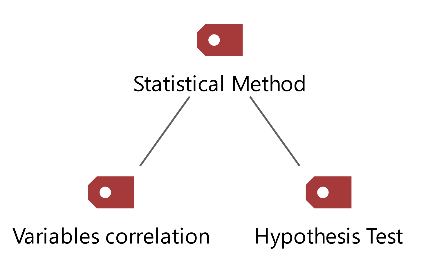
\includegraphics[width=12cm]{figuras/statistical_type.png}
		}{
			\Fonte{Produced by the author.}
		}	
	\end{figure}

\subsection{Resource data}
\label{subsec:results-resource-data}

In general, the papers do not present resource data of the experiments in the text. 19 experiments describe some information about the resource, as time-period, costs or human resources. Among this information, the time-period presented varies from 2 days to 6 months with the mean of 3 months-period. 4 experiments explain some information about cost, two of them chose some technology due to their low cost. One experiment says pay \$25 per hour to participants, and another pays \$60 for 3-hour sessions. One paper describes their team to apply the experiment. Almost always there is little or no information about the resources, this can hinder the replication of the experiment, as well as it lacks evidence to the descriptive text about adequacy, limits, qualities, costs and associated risks. Figure \ref{fig:resource_information} shows the resource information retrieved.


	\begin{figure}[h] 

   	    \captionsetup{width=12cm}%Da mesma largura que a figura
		\Caption{\label{fig:resource_information} Resource information}
		\UFCfig{}{
			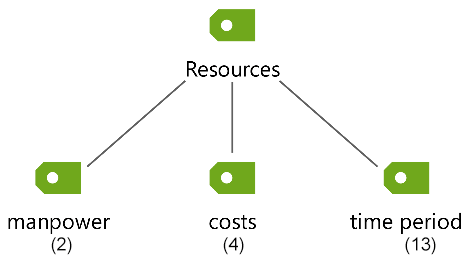
\includegraphics[width=12cm]{figuras/resource_information.png}
		}{
			\Fonte{Produced by the author.}
		}	
	\end{figure}

\subsection{Ethical Concepts}
\label{subsec:results-ethical-concepts}


The ethical concepts also are not well covered in the papers; even it is an essential step to produce an experiment with people who have disabilities \cite{Wohlin2000}. Among papers that threats the ethical concepts, 8 papers mentioned signing consents, two of them also applies to stop rules to enforcing ethical concept; 6 papers present the ethics council approved by legal institutions; two experiments express some information concern the user safety. It should be considered the local laws of ethical concepts and also the published year for each experiments. Figure \ref{fig:ethical_information} shows the sample information retrieved from each experiment. 

	\begin{figure}[h] 

   	    \captionsetup{width=12cm}%Da mesma largura que a figura
		\Caption{\label{fig:ethical_information} Ethical concepts}
		\UFCfig{}{
			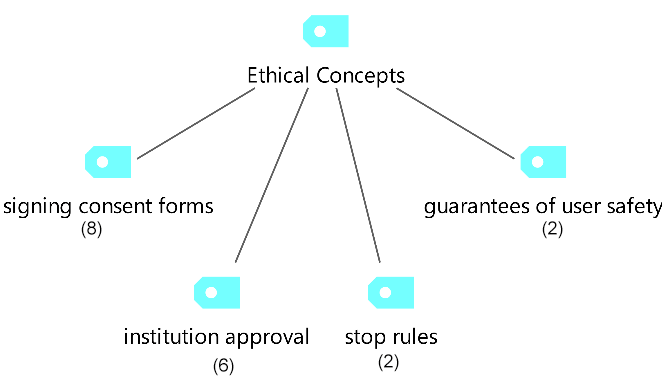
\includegraphics[width=12cm]{figuras/ethical_information.png}
		}{
			\Fonte{Produced by the author.}
		}	
	\end{figure}



\subsection{Hypothesis and groups}
\label{subsec:results-hypothesis}

Hypothesis is the basis for the statistical analysis of an experiment. A hypothesis is stated formally, and the data collected during the experiment is used to, if possible, reject the hypothesis \cite{Wohlin2000}. If the hypothesis can be rejected, then conclusions can be drawn, based on the hypothesis testing under given risks \cite{Wohlin2000}. Thus, the hypothesis is the core of the experiment design. Seeking to understand the hypothesis, we select which experiments have explicit in the text the Hypothesis and which of them test it. Even if the paper explains the research question or the goal of the experiment in the text, we do not count these. Wohlin divides the Hypothesis formulation from the Goal definition as two different phases of the experiment process. 

Figure \ref{fig:hypothesis} shows the two codes derived from this category. The ``Hypothesis well explicit'' is coded when the paper presents the hypothesis structured very well, as the experiments from ``Model of Cognitive Mobility for Visually Impaired'' \cite{Pissaloux2017TowardsDevices}.

	\begin{figure}[h] 

   	    \captionsetup{width=6cm}%Da mesma largura que a figura
		\Caption{\label{fig:hypothesis} Hypothesis}
		\UFCfig{}{
			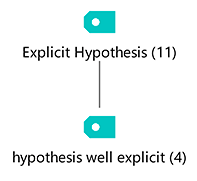
\includegraphics[width=6cm]{figuras/hypothesis.png}
		}{
			\Fonte{Produced by the author.}
		}	
	\end{figure}
	
\subsection{Variables}
\label{subsec:results-variables}

Almost no paper presents the variables explicitly in the text as dependent variables and independent variables. Thus, along with the text, we look for these variables to understand how the experiment is designed. After the grounded theory process, we produce three categories of dependent variables and three categories of independent variables. In searching this, we can see the variables are strongly related to the experiment hypothesis or objective when the hypotheses are not explicit in the text. As a result, Figure \ref{fig:variables__code_map} presents the code map generated and next we explain each variable structure.
\begin{landscape}
     	\begin{figure}[h] 

   	    \captionsetup{width=25cm}%Da mesma largura que a figura
		\Caption{\label{fig:variables__code_map} Variables code map}
		\UFCfig{}{
			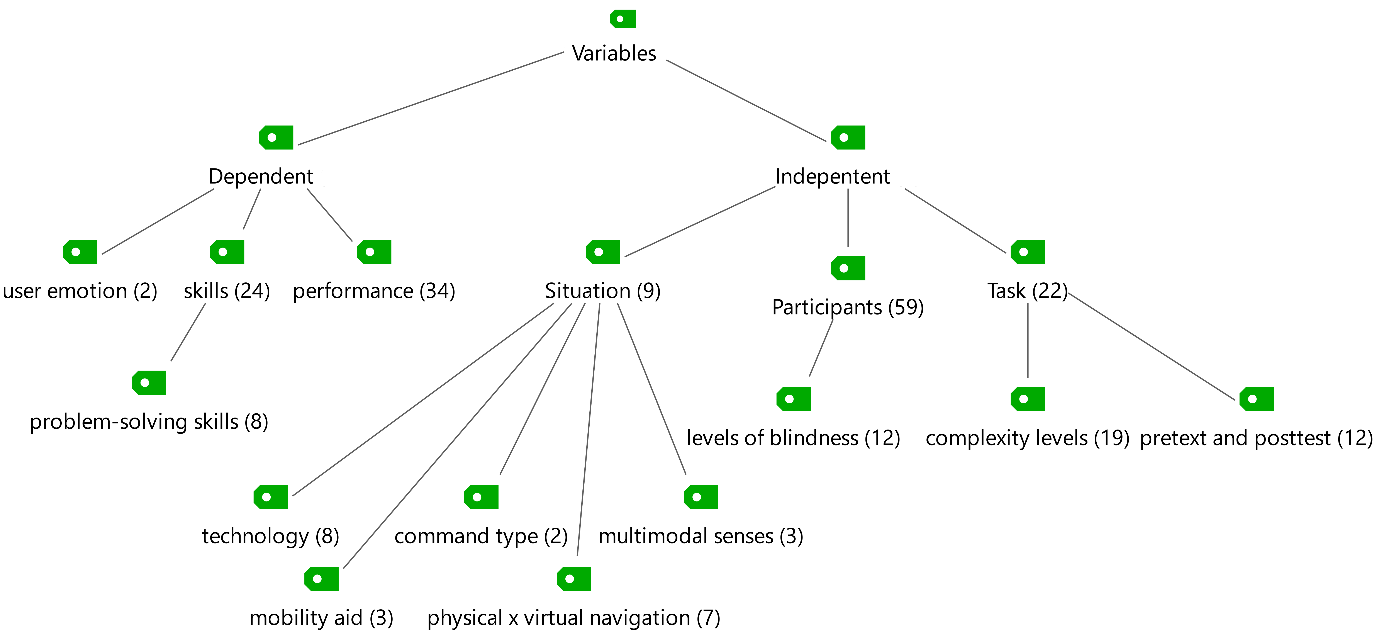
\includegraphics[width=25cm]{figuras/variables__code_map.png}
		}{
			\Fonte{Produced by the author.}
		}	
	\end{figure}
\end{landscape}

Dependent variables depend on how one or more independent variables influence or affect the participants in the experiment \cite{Wohlin2000}. As cognitive impact evaluation, the dependent variable is related to cognition processes. The main category of dependent variables is the task performance that has many ways to measure (explored in the Section \ref{subsec:results-measures}). We code as skills all dependent variables that work with a cognitive skill affected by some independent variable. Problem-solving skill stands out in the experiments and it turned a branching of skill. In the context, problem-solving, that can be understood as the act of consciously apply rules and procedures to bridge the gap between the initial problem state and a solution state \cite{Glatzeder2010}, involves solving, tasks and issues related to the application to users who are blind. Only two papers use some user emotion, as user opinion.

The independent variables are those variables that we can control and change in the experiment \cite{Wohlin2000}. So, they are related to domain knowledge. The independent variables encountered are characteristics of the situation, the participants and the tasks. The code map shows the categories that stand out in the data. Generally, the characteristics of the situation and tasks are factors, while participants characteristic are variables controlled, as etiology of blindness or age of participants. Nevertheless, usually, the levels of blindness are factors in the experiments used to divide the sample into groups \cite{Lee2014,Sanchez2000}.

Beyond the independent and dependent variables, we encountered in the grounded data other topics about the variables. 11 experiments have their variables well described in a separated section in the text. 8 experiments work with a control group to compare with the treatment. Also, three experiments stand out concern about the confounding variables. Report these topics shows more rigor in the controlled experiments, moreover it is not a usual practice.

\subsection{Tasks}
\label{subsec:results-tasks}

The tasks explored in the experiments are related to the technology assessed. Figure \ref{fig:tasks_code_map} shows the categories grounded in the experiment data. The two main categories are: Maps and Problem-Solving, this last was already discussed in the Variables section (Section \ref{subsec:results-variables}). As we have already presented in Section Technology, 31 experiments work with maps applications that aims to develop O\&M skills and other skills related. Not all presented in detail the tasks and measures, but we divide the Maps category into: \textit{(i)} location (indoor or outdoor maps), \textit{(ii)} number of spaces (one or more spaces), \textit{(iii)} known spaces (new or public spaces), \textit{(iv)} type (virtual or real map tasks), \textit{(v)} tasks that the participant need to reproduce a map using some modeling kit, as bricks, and \textit{(vi)} tasks that use the clock \cite{SanchezVideogaming}. Note, the same task of the experiment could have more than one code. 
\begin{landscape}
    \begin{figure}[h] 

   	    \captionsetup{width=25cm}%Da mesma largura que a figura
		\Caption{\label{fig:tasks_code_map} Tasks code map}
		\UFCfig{}{
			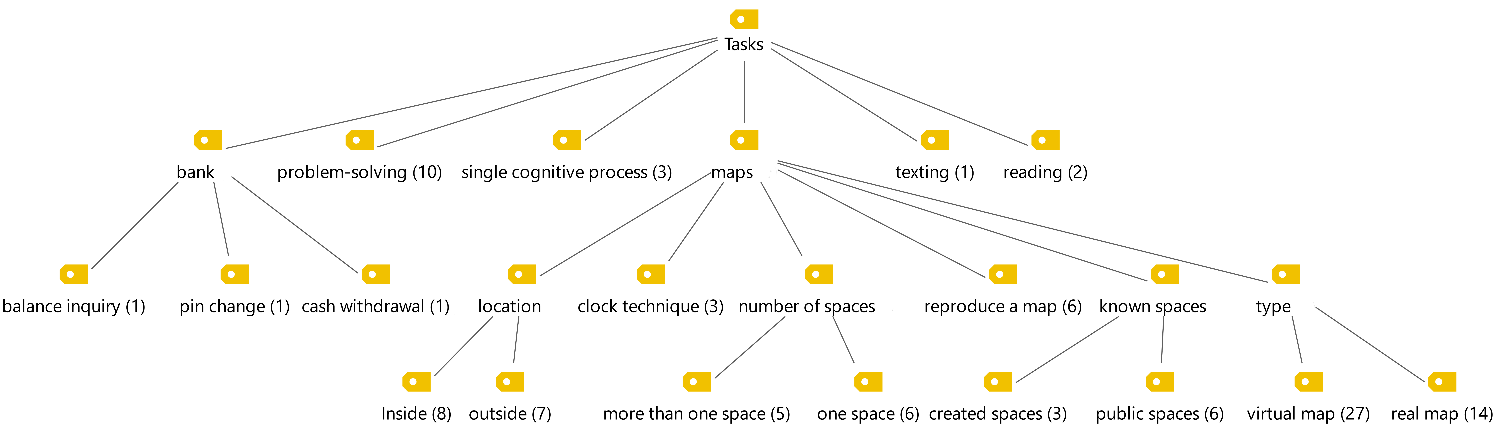
\includegraphics[width=25cm]{figuras/tasks_code_map.png}
		}{
			\Fonte{Produced by the author.}
		}	
	\end{figure}
\end{landscape}
	
\subsection{Measures}
\label{subsec:results-measures}

The measures are defined according to the variables of the experiment. Figure \ref{fig:measures_code_map} shows the Measures code map grounded in data of the experiments. We find five categories, that are measures based on \textit{(i)} technology, \textit{(ii)} activity type, \textit{(iii)} tests, \textit{(iv)} user behavior, and \textit{(v)} task performance. The categories ``activity type'' and "task performance" highlight in front of the others because they are the most used. The ``activity type'' depends on the technology domain and the variables defined. For example, one measure defined to a map task is the obstacle detection \cite{Merabet2016}. The task performance measures are the most important cognitive measures because they can be used in several domains, for example, time duration and error rate.

\begin{landscape}
	\begin{figure}[h] 

       \captionsetup{width=25cm}%Da mesma largura que a figura
	\Caption{\label{fig:measures_code_map} Measure code map}
	\UFCfig{}{
		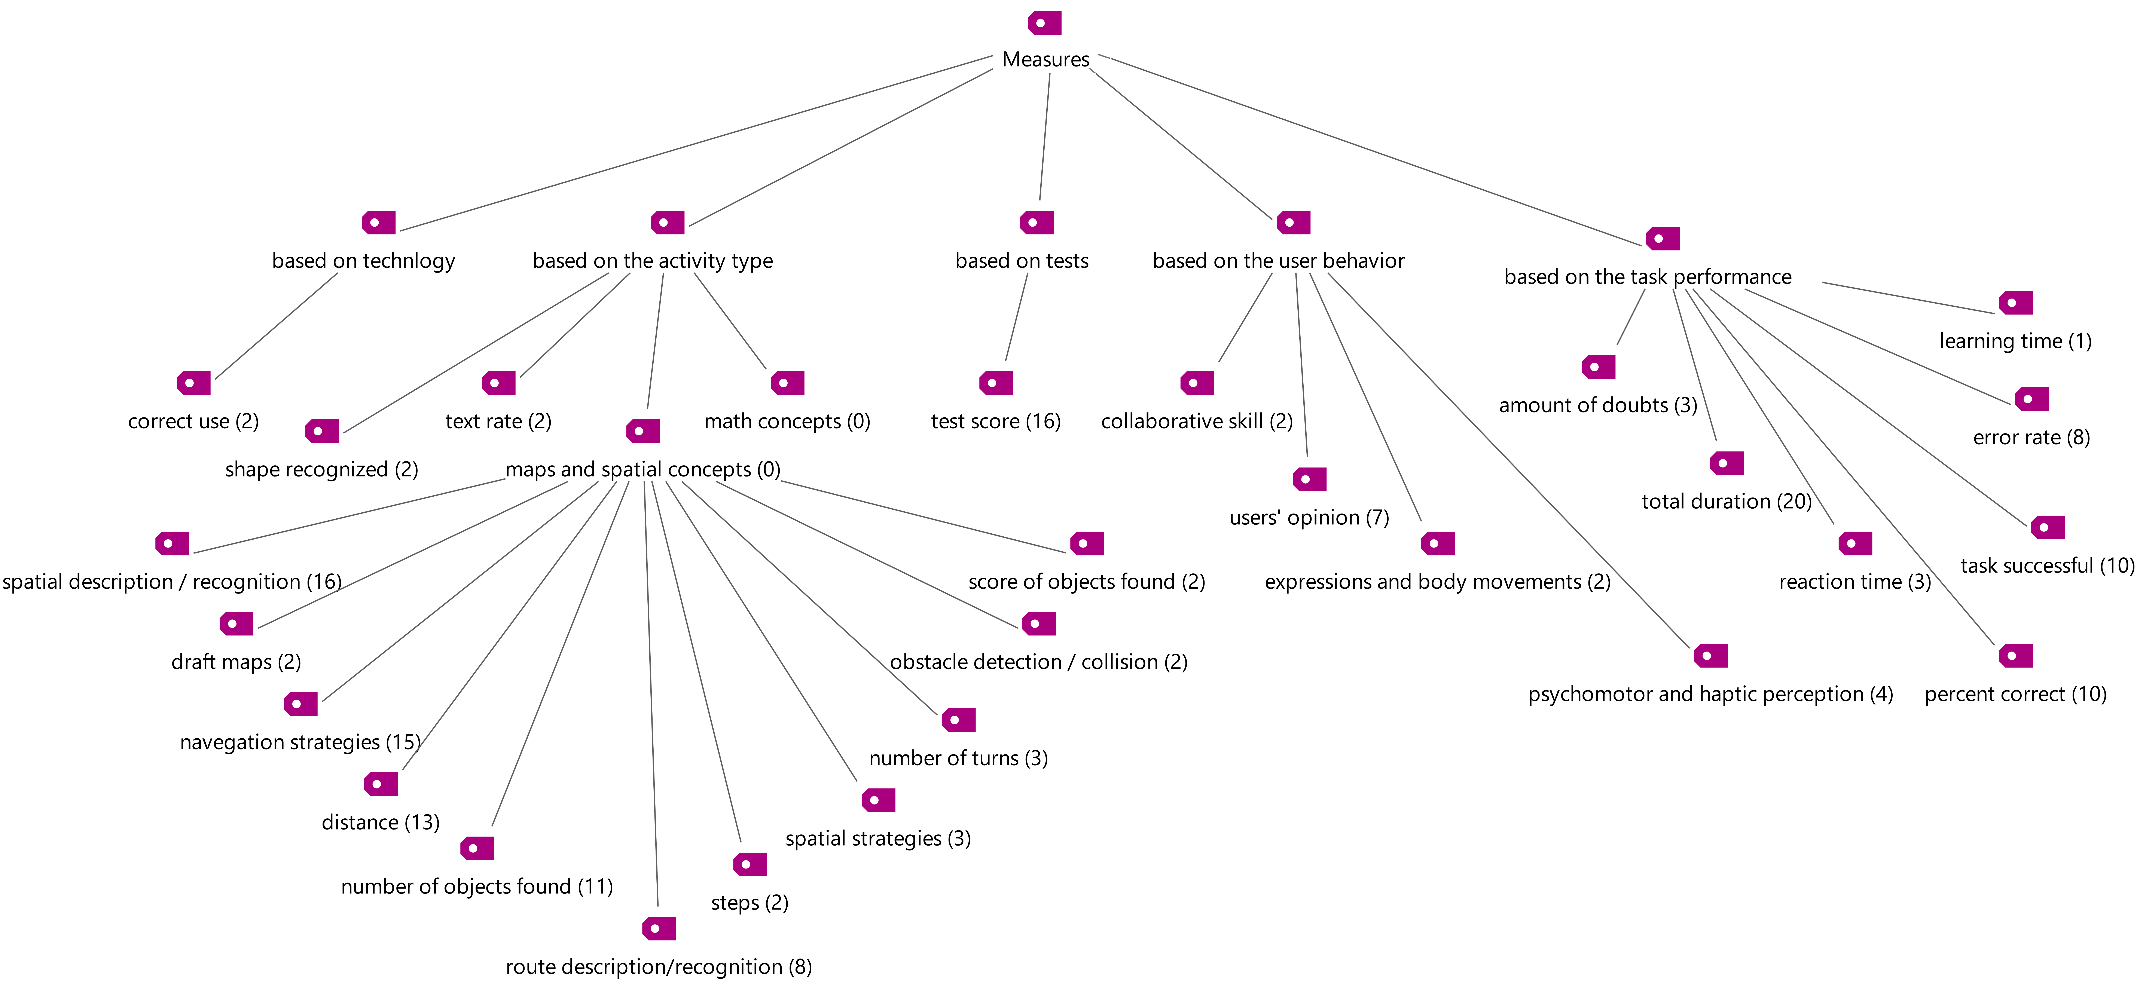
\includegraphics[width=25cm]{figuras/measures_code_map.png}
	}{
		\Fonte{Produced by the author.}
	}	
	\end{figure}
\end{landscape}

\section{Theory of Cognitive Impact Evaluation}
\label{sec:results-theory}

After organizing the core category and related the concepts of Cognitive Impact Evaluation, the data was arranged to observe the excerpts related to each concept. The relations found were identified by analyzing patterns and implicit meaning between codes. Once the concepts are related they were organized into a theoretical framework \cite{Corbin1998}, meaning the representation of concepts, together with their definitions and relations among them. Figure \ref{fig:central_idea_of_cognitive_impact} presents the cognitive impact evaluation central idea, considering the context of multimodal interfaces for people who are blind or visually impaired.

	\begin{figure}[h] 

   	    \captionsetup{width=16cm}%Da mesma largura que a figura
		\Caption{\label{fig:central_idea_of_cognitive_impact} Central idea of cognitive impact evaluation for blind users}
		\UFCfig{}{
			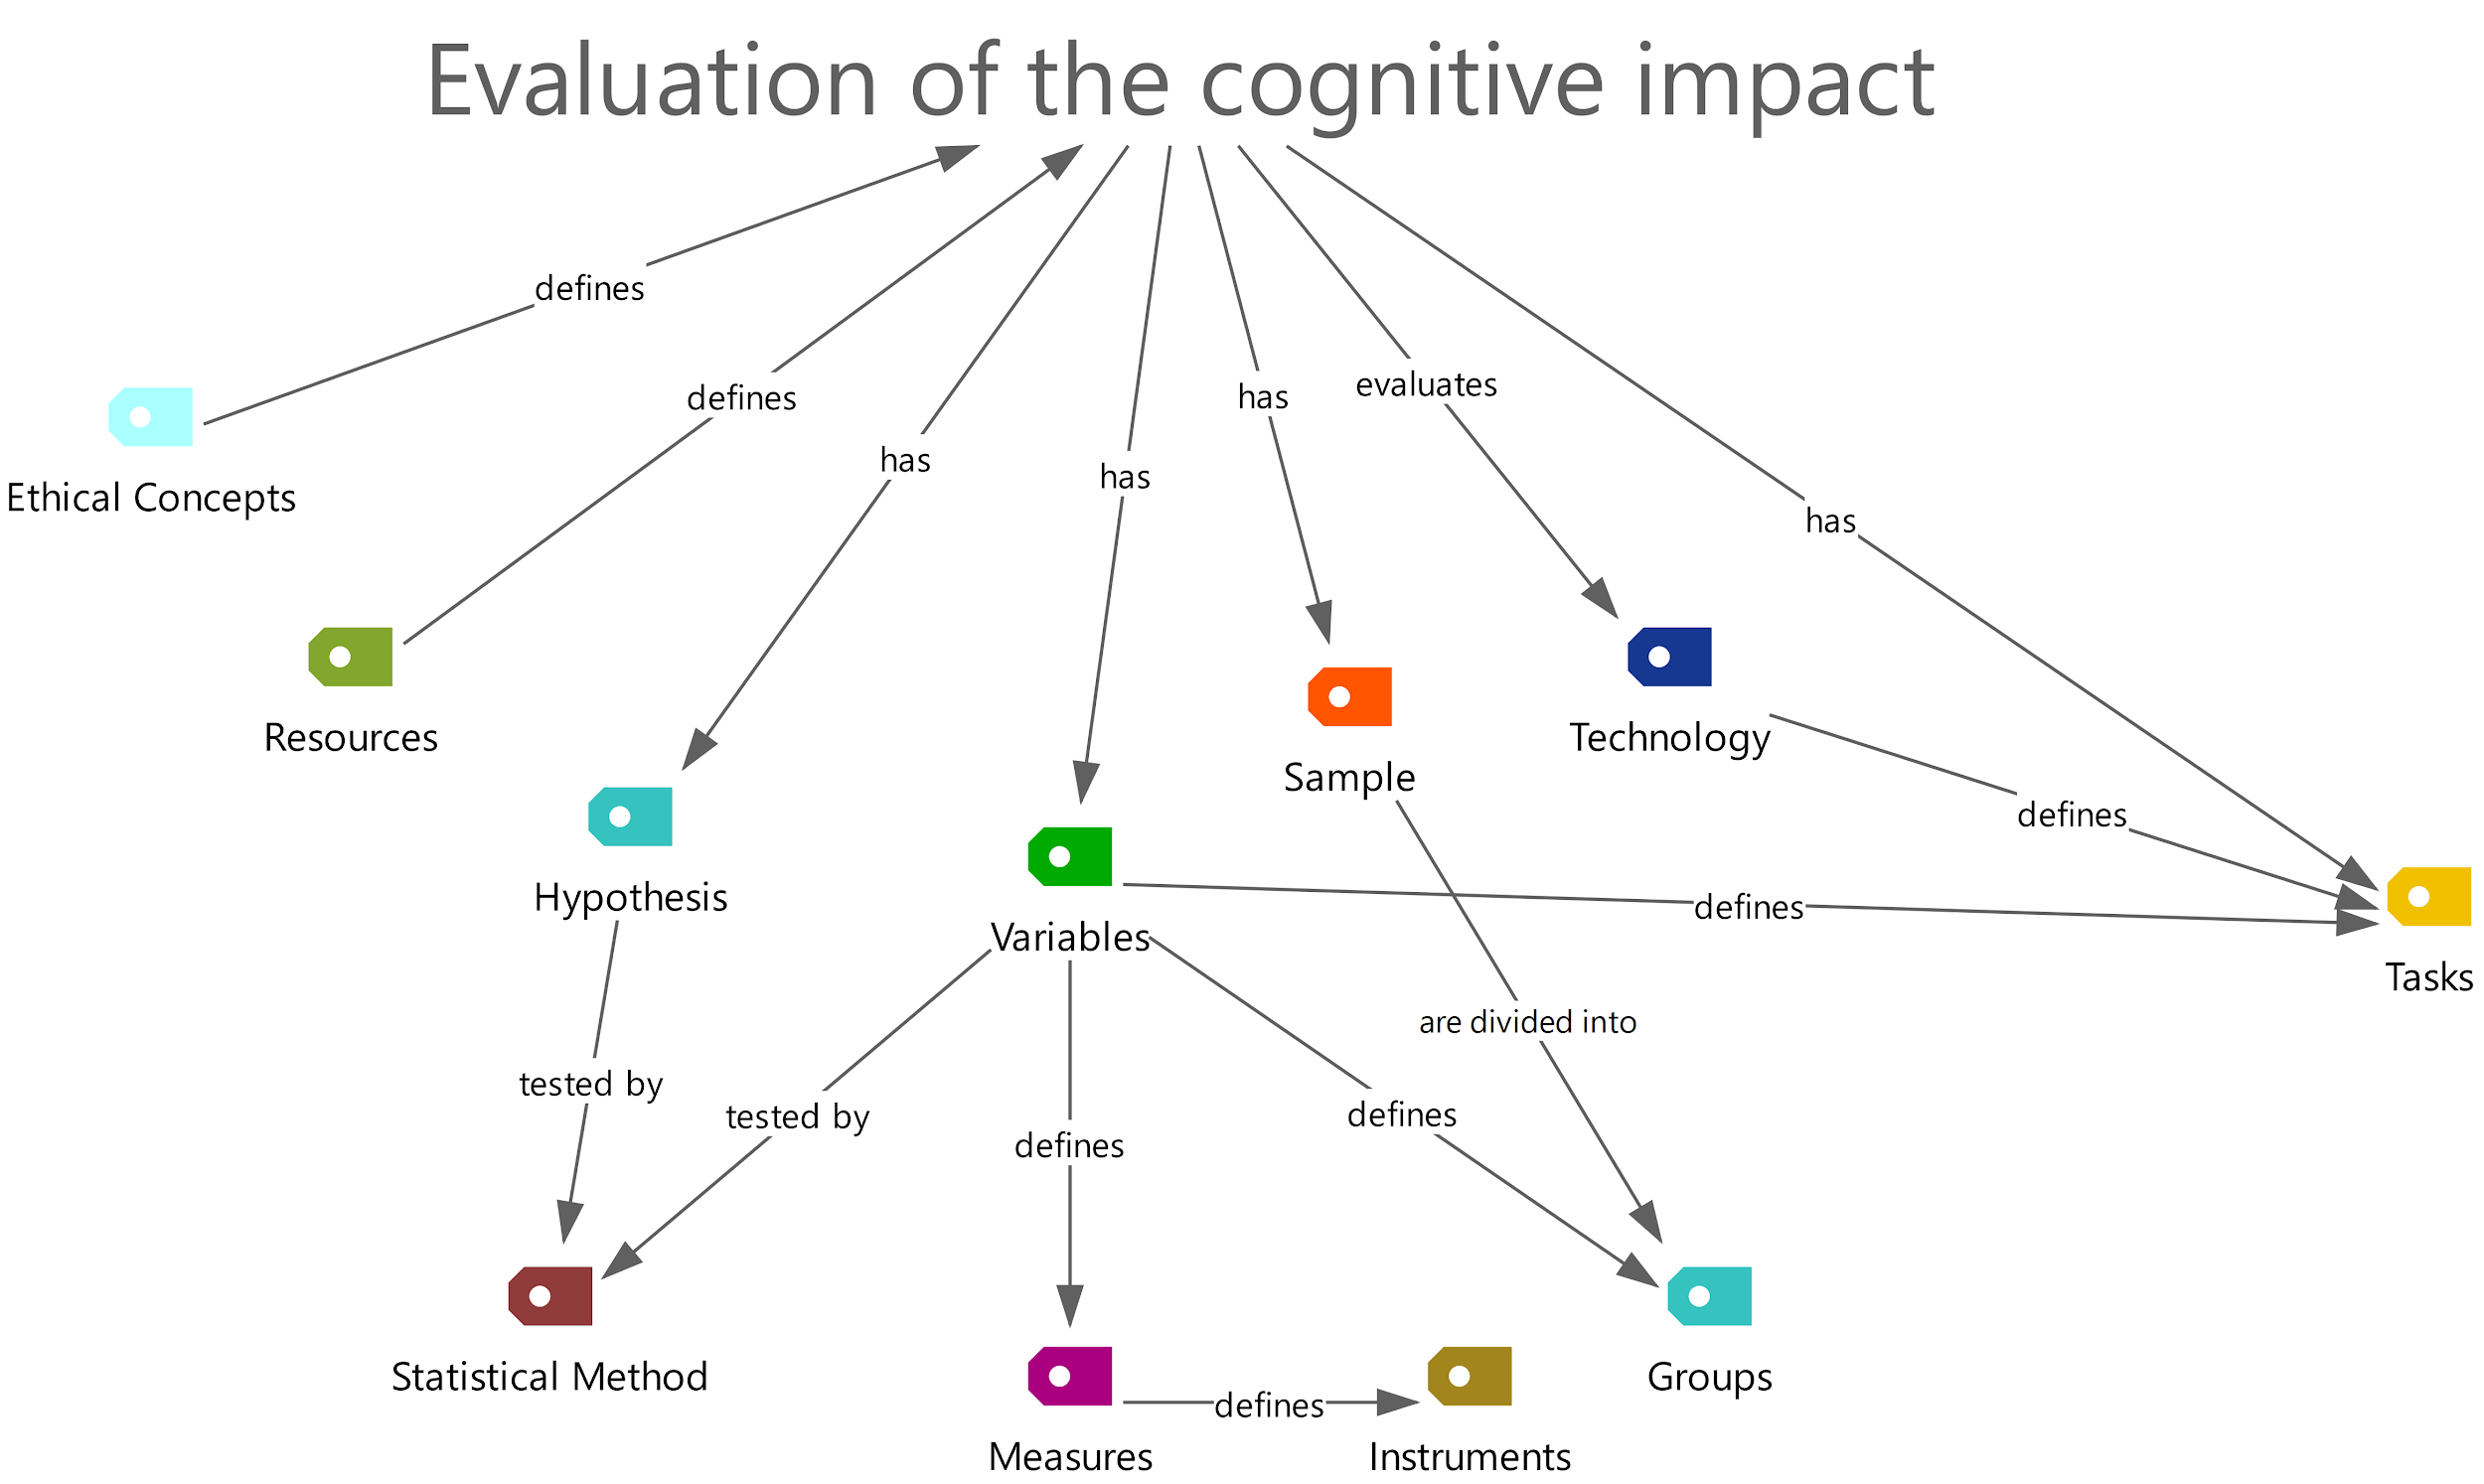
\includegraphics[width=16cm]{figuras/central_idea_of_cognitive_impact.png}
		}{
			\Fonte{Produced by the author.}
		}	
	\end{figure}

	\chapter{Guidelines}
\label{chap:guidelines}
\addtocontents{toc}{\protect\setcounter{tocdepth}{1}}

In this chapter, we present the guidelines proposed in this master thesis based on results from the Systematic Literature Review and Grounded Theory. Section \ref{sec:guidelines-overview} presents an overview of guideline structure. The next sections (\ref{sec:guidelines-G1}, \ref{sec:guidelines-G2}, \ref{sec:guidelines-G3}, \ref{sec:guidelines-G4}, \ref{sec:guidelines-G5}) present the guidelines one by one in the structure presented in Section \ref{sec:guidelines-overview}.

\section{Overview}
\label{sec:guidelines-overview}

The analysis of all data extracted shows the necessity of some rules to follow when conducting an experiment in the context of this study. The methodology used to reach the Guidelines is based on evidence by using Systematic Literature Review and Grounded Theory. The Systematic Literature Review retrieved information about the experiments executed in this area and gave us information about how the experiments are commonly applied. The Grounded Theory deepened in this information which made possible to compare what happens and what is recommended by the literature.



The five guidelines are: \nameref{sec:guidelines-G1}, \nameref{sec:guidelines-G2}, \nameref{sec:guidelines-G3}, \nameref{sec:guidelines-G4}, \nameref{sec:guidelines-G5}). The appendix \ref{ap:guidelines} presents an overview of each guidelines in the form of an infographic. An overview of the guidelines  Following some examples used in software engineering \cite{Kappel2006DevelopingMenus,Kitchenham2002PreliminaryEngineering}, we came up with the guidelines structure to evaluate the cognitive impact composed of seven parts, described as follows:
    \begin{enumerate}
        \item \textbf{When:}  In this part, we explain in which step this guideline can help. The steps are based on the five phases and steps of the experimental process described by \citeonline{Wohlin2000}.
        \item \textit{\textbf{Why:} In this part, we explain the guideline based on the scientific literature on Cognitive Psychology and Experimentation in Software Engineering.
        \item \textbf{How:} In this part, we explain how to apply the guideline in detail.
        \item \textbf{Example} In this part, we present a real example of a paper retrieved from the Systematic Literature Review.
        \item \textbf{Priority:}} In this part, we give a priority note (from 0 to 5) according to the importance of the guideline and with the problems that were found in the experiments studied.
        \item \textbf{Findings:} In this part, we present the main findings from our methodology (Systematic Literature Review and Grounded Theory) that have led to that guidelines.
        \item \textbf{Attachments:} It is an optional part where we show some graph or table to guide the rules presented.
    \end{enumerate}


\section{\textit{G1} - Specify the Hypotheses}
\label{sec:guidelines-G1}

\noindent \textit{\textbf{When:}}  In the Planning phase of the experiment process, in the Hypothesis Formulation step.
\vspace{5mm}


\noindent \textit{\textbf{Why:}} In the context of cognitive impact evaluation of multimodal interfaces for people who are blind, the experiments assume the technologies used has a cognitive impact on its users. This theory should be tested to see if it has the power to predict certain aspects of the phenomena with which it deals. Thus, the hypothesis has to be stated clearly since the Scoping phase. Even if particular findings appear to confirm a given hypothesis, the findings must be subjected to statistical analysis to determine their statistical significance and to retain or reject hypotheses \cite{Sternberg2011}. In addiction, \citeonline{Kitchenham2002PreliminaryEngineering} presents the shallow hypotheses concept, when the hypothesis is simply a statement of the tests to be performed, thus it does not reflect an underlying, explanatory theory. This represents the care that must be taken in the decision.
\vspace{5mm}

\noindent \textit{\textbf{How:}} Two kinds of hypotheses have to be formulated: a null hypothesis, states that there are no real underlying trends or patterns in the experiment setting; and alternative hypotheses, that are the hypotheses in favor of which the null hypothesis is rejected.  Choose one statistical test to evaluate the outcome of an experiment. More commonly, however, researchers use various statistical means of analyzing the data \cite{Sternberg2011}. The description of both null and alternative hypotheses should be as formal as possible \cite{Jedlitschka2007}.
%Table X\todo{} presents the most common statistical methods. 
\vspace{5mm}

\noindent \textit{\textbf{Example:}} The study ``Navigational 3D audio-based game-training towards rich auditory'' \cite{Balan2014} works with the hypothesis that the occipital visual cortex is not completely visual and that it shares functionality with other perceptual modalities. The researchers had used the Student t-test as a statistical method to test the hypothesis. As a result, the paired average from experiments proved to be non-significant (p=0.3 at p<0.01), and they reject the null hypothesis. These results lead to the hypothesis that the players could have rendered the audio data into a visual, imaginary representation of the virtual setting.
\vspace{5mm}

\noindent \textit{\textbf{Priority:}} 5/5
\vspace{5mm}

\noindent \textit{\textbf{Findings:}} Only 11 experiments from 52 experiments retrieved presented the hypothesis of the experiment in the text, among them, only 4 presented well, as a specific section to show the hypothesis or showed the null hypothesis beyond the general purpose of the study.
\vspace{5mm}

\section{\textit{G2} - Define and report the experiment variables}
\label{sec:guidelines-G2}

\noindent \textit{\textbf{When:}} 
In the Planning phase of the experiment process, in the Variable Selection step, and in the Presentation \& package phase.
\vspace{5mm}

\noindent \textit{\textbf{Why:}} In any controlled experimental designs, the variables should relate to many cognitive aspects of the experimental situation are controlled. There are two kinds of variables need to be described: dependent and independent variables. Independent variables are those variables that we manipulate in the experiment to see the factors influence in the phenomena \cite{Wohlin2000}, while other aspects of the investigation are held constant (control variables). Dependent variables are outcome responses, the values of which depend on how one or more independent variables influence or affect the participants in the experiment \cite{Sternberg2011}. Often there is only one dependent variable, and it should, therefore, be derived directly from the hypothesis \cite{Wohlin2000}.

Different from Software Engineering literature, the Cognitive Psychology evaluation process insert a new concept, the irrelevant variables. The confounding variables are a type of irrelevant variable that has been left uncontrolled in a study. When conducting research, we must be careful to avoid the influence of confounding variables. Treatment is one particular value of an independent variable manipulated. When the experimenter manipulates the independent variables, he or she controls for the effects of irrelevant variables and observes the effects on the dependent variables (outcomes). These irrelevant variables that are held constant are called control variables \cite{Sternberg2011}. 

In the context of cognitive evaluation and based on systematic literature review findings, we present the merge of these two approaches in Figure \ref{fig:central_idea_of_cognitive_impact2}.

	\begin{figure}[h] 

   	    \captionsetup{width=10cm}%Da mesma largura que a figura
		\Caption{\label{fig:central_idea_of_cognitive_impact2} Relation between variables}
		\UFCfig{}{
			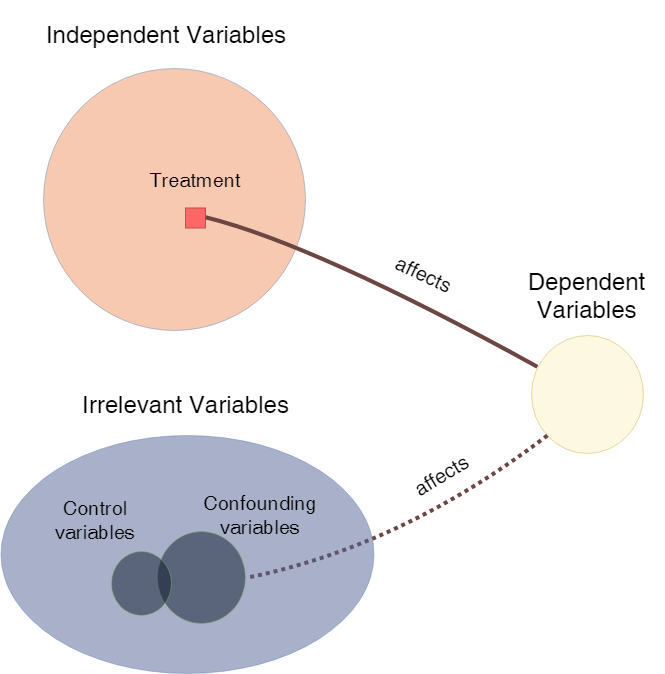
\includegraphics[width=10cm]{figuras/central_idea_of_cognitive_impact2.png}
		}{
			\Fonte{Produced by the author.}
		}	
	\end{figure}
\vspace{5mm}

\noindent \textit{\textbf{How:}} First, the variables must be understood and defined in the planning phase. We recommend the classification proposed above that is clear about the type of variable. Despite it is most important to select variables following the purpose of the experiment, the Variables code map (see Figure \ref{fig:variables__code_map}) presents a range of possible variables. Use this range to guide through the choice.

It is essential not only to identify appropriate contextual variables but also to measure them consistently \cite{Kitchenham2002PreliminaryEngineering}. The Measures code map (see Figure \ref{fig:measures_code_map}) presents a range of possible measures. To measure, check specific instruments in the literature that have already been used before. There are several surveys, checklists, checklists, questionnaires, kits and logs used in literature and the uses of published instruments turns the experiment more rigor. In the attachments of this guideline, we present a practical example of how to describe the variables in the experiment. Building a pattern for results provides a consistent basis for comparing and classifying cognitive impact.
\vspace{5mm}

\noindent \textit{\textbf{Example:}} The study ``Construction of cognitive maps of unknown spaces using a multisensory virtual environment for people who are blind''\cite{Lahav2008b} defines the experiment as follow:
\begin{description}
    \item[Dependent Variable] Navigation performance (relate to the participants’ cognitive map of the explored space):
    
   \begin{enumerate}[label=\alph*.]
       \item	cognitive map structural components: Eight variables related to the cognitive map structural components referred to the accurate mapping of spatial structure information.
       \item	spatial relationships estimation: (1) references creation, (2) directions estimation, and (3) distances estimation.
       \item	cognitive map construction process: Spatial strategy, Spatial model used, Chronology of the descriptive process 
   \end{enumerate}
   
   \item[Independent Variable] level of blindness, gender, age, Maps abilities, language spoken, onset of blindness, assistive aid, other disabilities.
   
   \item[Factor] Experimental group (21 participants) x control group (10 participants), type of environment explored (the MVE and the real space).
   
\end{description}

Eight variables related to the cognitive map structural components referred to the accurate mapping of: (1) room size, (2) room shape, (3) structural components (e.g., doors, windows), (4) structural component location, (5) objects within the room (e.g., boxes, cubes), (6) object location, (7) object size, and (8) object position. Three variables were related to spatial relationships estimation: (1) references creation (e.g., landmarks, spatial relations – behind, nearby), (2) directions estimation (e.g., to the north, room’s center), and (3) distances estimation (e.g., close-to, steps).

The study defines two groups that were similar in gender, age, and age of vision loss (congenitally blind or late-blind). The experimental group included 21 participants who explored the unknown space by means of the MVE. The control group included 10 participants who explored the unknown space by actual navigation in the real space.
\vspace{5mm}

\noindent \textit{\textbf{Priority:}} 5/5

\noindent \textit{\textbf{Findings:}} In cognitive impact experiments, the dependent variables are related to performance or cognitive skills, and some of them works with user emotions as dependent variables.

%11 experiments have their variables well described in a separated section in the text. 8 experiments work with a control group to compare with the treatment.

% we produce three categories of dependent variables and three categories of independent variables. In searching this, we can see the variables are strongly related to the experiment hypothesis or objective when the hypotheses are not explicit in the text.
 
\vspace{5mm}

\noindent \textbf{Attachments:} Table \ref{tab:schema_for_description_of_variables} presents schema to describe the variables. The name of the variable could have a code to be referenced later. The type of the variable could be independent, dependent, irrelevant or more detailed as shown in Figure \ref{fig:central_idea_of_cognitive_impact2}. The abbreviation could be a simple name from the hole name. The variables can be divided into three different classes: product, process, and resource. The process describes which activities that are needed to produce the software. The products are the artifacts, deliverables or documents that results from a process activity. Resources are the objects, such as personnel, hardware, or software, needed for a process activity \cite{Wohlin2000}. The entity is the instance of the class. The type of attribute could be internal, that can be measured purely in terms of the object, or external, that can only be measured with respect to how the object relates to other objects. The scale type could be nominal, ordinal and others. Beyond the scale type, the table presents the unit and the range for nominal and restricted ordinal scales it should present the definition of each scale point. And finally the counting rule in the context of the entity.
%%%%%Comentário do .doc%%%%
%refazer um próprio com foco no tipo de avaliação prevista%

\begin{table}[h]
	\captionsetup{width=16cm}%Deixe da mesma largura que a tabela
	\Caption{\label{tab:schema_for_description_of_variables} Schema for description of variables}%
	\IBGEtab{}{%
		\begin{tabular}{m{1.3cm}m{1.5cm}m{1.3cm}m{1.2cm}m{1cm}m{1.3cm}m{1.1cm}m{.5cm}m{1.7cm}m{1cm}}
			\toprule
		    Name of the variable & Type of the variable & Abbreviation & Class & Entity & Type of attribute & Scale type & Unit & Range & Counting rule \\
%			\midrule \midrule
			\bottomrule 
		\end{tabular}%
	}{%
	\Fonte{Adapted from \citeonline{Jedlitschka2007}.}%
%	\Nota{esta é uma nota, que diz que os dados são baseados na	regressão linear.}%
%	\Nota[Anotações]{uma anotação adicional, seguida de várias outras.}%
    }
    \end{table}
%%%% figura excluida e comentada %%%%
\begin{comment}
	\begin{figure}[h] 

   	    \captionsetup{width=16cm}%Da mesma largura que a figura
		\Caption{\label{fig:schema_for_description_of_variables} Schema for description of variables }
		\UFCfig{}{
			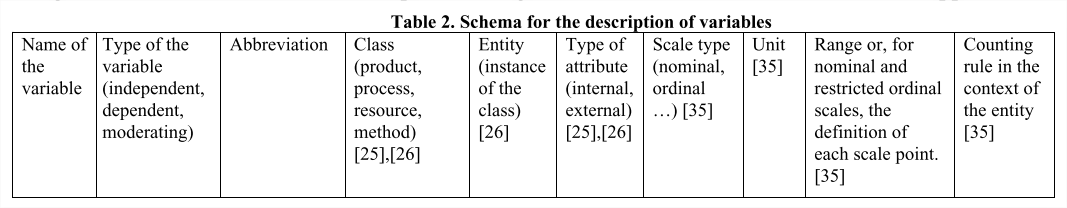
\includegraphics[width=16cm]{figuras/schema_for_description_of_variables.png}
		}{
			\Fonte{Adapted from \citeonline{Jedlitschka2007}.}
		}	
	\end{figure}
\end{comment}
\vspace{5mm}

\section{\textit{G3} - Choose a valid sample}
\label{sec:guidelines-G3}

\noindent \textit{\textbf{When:}}  
In the Planning phase of the experiment process, in the Hypothesis Formulation step. 
\vspace{5mm}

\noindent \textit{\textbf{Why:}} The selection of subjects, also called a sample, is closely connected to the generalization of the results from the experiment. With the objective of generalizing the results to the desired population, the selection must be representative of that population \cite{Kitchenham2002PreliminaryEngineering}. \citeonline{Wohlin2000} presents two sampling categories, the probability, and the non-probability, and give three examples from each sampling techniques. Among these examples, the most sample encountered in the impact experiments in the context of this work are Simple random sampling (subjects are selected from a list of the population at random) and Convenience sampling (the nearest and most convenient persons are selected as subjects). Other examples could be read in \citeonline{Wohlin2000}.

The size of the sample also impacts the generalization of the results. The size of the sample affects the error rate, and it is closely related to the power of the statistical test \cite{Wohlin2000}. Wohlin presents some general principles for choosing the sample size:

\begin{quotation}
     If there is significant variability in the population, the larger sample size is needed. And the analysis of the data may influence the choice of the sample size.
\end{quotation}

Moreover, all participant characteristics that might have an effect on the results or restrict the sample in some way should be well described in the experiment report \cite{Jedlitschka2007}. For the subjects who are blind or visually impaired, the following characteristics must take account in the sampling selection, and in the report: blindness level, blindness onset, and etiology of blindness.

Concerning the blindness level, there are many definitions about it. In general, the experiments use the categories of ``Blindness and Deafness'' \cite{WHO2018Blindness}. This institution defines two categories: blind and visually impaired. Different from this concept of the blind, some papers call the participants as legally blind, which depends on the country laws and are broader than blind (see Section \ref{subsec:background-blindness}). Some of the experiments present blindfolded participants or even blindfolded the visually impaired participants to equal the visual acuity. The participation of sighted blindfolded subjects is interesting to compare results; however, this set does not present the real perception of a blind subject, mainly in cognitive aspects.
%TODO encontrar essa referência

The blindness onset (the time with impairment) and its etiology are characteristics that should take into account because this could affect the results.  Given the enormous variety of possible combinations with these characteristics, most of the papers report the characteristics and assume as threats to validity. Confounding variables touching these characteristics could be controlled in the sampling choice.

The sample selection may include experience with the technology or mean/range of experience in years, or educational level \cite{Shull2008GuideEngineering}. Concerning a skill of subjects, a good approach has used a pre-test to capture the experience and divide the subjects into groups. 

In the experiment report, the sampling strategy and the resulting samples need to be described, including the number of participants (per condition), the kind of participants (e.g., computer science students), and the populations from which they were drawn \cite{Jedlitschka2007}.
\vspace{5mm}

\noindent \textit{\textbf{How:}} In the planning phase, experimenters must plan to use a representative sample of the population of interest. In this point, there are the following topics.
\begin{enumerate}
    \item \textbf{Number of users:} choose as larger as possible in resources available and preferably the size no less than 6 persons This number is grounded evidence-based information from the Systematic Literature Review where most of the experiments have presented from 6 to 10 participants.
    \item \textbf{Blindness level distribution:} choose the blindness level distribution according to the variables of the experiment. Do not use only sighted blindfolded participants, since they do not represent the cognitive perception of a blind person. However, if the visual feedback is significant to accomplish the task, when possible, blindfold all participants to equal the visual acuity. When there are sighted persons, balance the number of sighted and blind participants.
    \item \textbf{Sampling technique:} prioritize the use of simple random sampling.
\end{enumerate}
    %\item \textbf{Gender information:} We suggest balancing in the sample the number of each gender, female and male.
    %\todo{RETIRADO Gender information We suggest balancing in the sample the number of each gender, female and male.}

All this information needs to be described in detail. We suggest putting all information in a table careful to not identify the participants. Do not forget the age, gender and blindness level.
\vspace{5mm}

\noindent \textit{\textbf{Example:}} The study ``Assessment of feedback modalities for wearable visual aids in blind mobility''\cite{Adebiyi2017} has a sample with 23 users, among them 12 are blind, and 11 are visually impaired. They present in each blindness level group the gender and the age range. Moreover, the experiment reports a table with code, age, gender and diagnosis of Vision Loss. 
\vspace{5mm}

\noindent \textit{\textbf{Priority:}}  4/5
\vspace{5mm}

\noindent \textit{\textbf{Findings:}} One experiment does not inform the number of users. Moreover, 7 experiments do not inform the age of participants. The majority of experiments works with convenience sampling. We suppose that this happens because the kind of population involved, which is restricted to people who are blind or visually impaired. 9 experiments do not inform the proportions of the blind, low vision, sighted and blindfolded. 16 experiments do not inform the gender distribution. Gender is equilibrated. Only 3 experiments have used random groups.
\vspace{5mm}

\section{\textit{G4} - Plan and Report Ethical Concepts}
\label{sec:guidelines-G4}
\vspace{5mm}

\noindent \textit{\textbf{When:}}  
In the Planning phase of the experiment process, in the Selection of Subjects step and the Presentation \& package phase.
\vspace{5mm}

\noindent \textit{\textbf{Why:}} In contrast, the ethical issues raised by empirical methods have received little attention in the software engineering literature \cite{Vinson2008AHumans}. Any empirical research activity involving human subjects must consider ethical aspects \cite{Wohlin2000}.  Based on \cite{Vinson2008AHumans}  the experiment must have:
\begin{itemize}
    \item \textbf{Ethical review:} Legislation of some countries requires an ethical review for studies involving human subjects. Some types of study in Software Engineering do not need to have an ethical review, but in the context of Cognitive Impact, the experiment should have an ethical review.
    \item \textbf{Informed consent:} The basis for a human-oriented empirical study (e.g., an experiment) is that subjects are participating voluntarily and that they have enough information to decide to participate or not.
    \item \textbf{Confidentiality:} The subjects must be sure that any information they share with researchers will remain confidential, which includes data privacy, data anonymity, and anonymity of participation. The researchers must lead to publishing their results without harming the companies’ and individuals’ integrity.
    \item \textbf{Sensitive results:} Outcomes from an empirical study may be sensitive in different respects for different stakeholders, that should be participants and institutions, as universities or enterprises involved.
    \item \textbf{Inducement:} In recruiting subjects for an experiment, there must be inducements to motivate their participation. However, the value should not be too large, since this could cause people to participate merely to receive the inducement.
    \item \textbf{ Feedback:} To maintain long-term relationships and trust with the subjects of a study, feedback of results and analysis are important.
    
\end{itemize}
\vspace{5mm}

\noindent \textit{\textbf{How:}} The experimenters must have to look at the ethical concepts when preparing the subjects groups. First, send the ethical review to the institution responsible in your jurisprudence. When calling a participant, present the informed consent to sign. Remember that the consent must be read to a participant who is blind, and he/she should sign with a witness, if the consent is not accessible, such as on printed paper. Take care of the sensitive results, following the procedures approved in the ethical review. Do not forget citing the ethical review and informed consent when reporting.
\vspace{5mm}

\noindent \textit{\textbf{Example:}} The study ``Virtual environments for the transfer of navigation skills in the blind: a comparison of directed instruction vs. video game based learning approaches'' \cite{201449} presents the stop rules for enforcing ethical concept, written consent, and procedures approved by the Massachusetts Eye and Ear Infirmary.
\vspace{5mm}

\noindent \textit{\textbf{Priority:}} 5/5
\vspace{5mm}

\noindent \textit{\textbf{Findings:}} 9 experiments express some information concern the ethical concepts. They explain Signing consent forms (8), stop rules (2), institutions approval (6) and user safety (2).
\vspace{5mm}

\section{\textit{G5} - Specify the resources available to all parties involved}
\label{sec:guidelines-G5}

\noindent \textit{\textbf{When:}}  
In the Planning phase of the experiment process, in the Context Selection step and the Presentation \& package phase.
\vspace{5mm}

\noindent \textit{\textbf{Why:}} In software development organizations, methods and tools are employed that frequently lack sufficient evidence regarding their suitability, limits, qualities, costs, and associated risks \cite{Vinson2008AHumans}. Regarding this, the experiment must be clear about their resources and how it leads to threats of validity. \citeonline{Jedlitschka2007} say to describe the impacts with regard to cost, schedule, and quality, circumstances under which the approach presumably will not yield the expected benefit.
\vspace{5mm}

\noindent \textit{\textbf{How:}} In the Context Selection step, the researchers should plan the time, human resources and costs available. In the Presentation and Package phase, the researcher should explain when the experiment occurs and how long are the execution of the whole or each stage. The costs are interesting mainly when the participants receive money because it could impact the experiment.
\vspace{5mm}

\noindent \textit{\textbf{Example:}} The study ``Timbremap: Enabling the Visually-Impaired to Use Maps on Touch-Enabled Devices'' \cite{Su2010} works present the scheduled for evaluating session (3-hour), and honorarium for their time granted for participants (\$60).
\vspace{5mm}

\noindent \textit{\textbf{Priority:}} 2/5
\vspace{5mm}

\noindent \textit{\textbf{Findings:}} 19 experiments describe some information about the resource, as time or costs. Only 4 experiments explain some information about cost. 1 experiment says pay \$25 per hour to participants; other pays \$60 for 3-hour sessions. 1 paper describes their team to apply the experiment.
\vspace{5mm}
	\chapter{Conclusion}
\label{chap:conclusion}

% O que me chamou a atenção na conclusão foi que vc coloca a metodologia como introduzida por vc e não foi, revisão sistemática com uso de grounded thoery não é contribuição sua. Suavize isso, por favor na conclusão e em toda a tese, se vc tiver feito algo nesse sentido. A sua contribuição está na aplicação delas para o seu tema e os resultados que encontrou.
% O meu ponto é que vc não pode considerar a metodologia como sua contribuição, ela já existe. O que vc fez foi aplicá-la em  um domínio específico, esta é sua contribuição secundária. Sua contribuição principal são os resultados da revisão sistemática e a análise dos dados com a grounded theory. Ficou mais claro?

The present chapter concludes the master's thesis, synthesizing the contributions obtained in this research, following the organization described next. Section \ref{sec:conclusion-summary} gives an overview of the research. Section \ref{sec:conclusion-mainresults} summarizes the main results of the research. Section \ref{sec:conclusion-contributions} presents the main contributions as also papers published. \ref{sec:conclusion-limitations} discusses the limitations of this work. Finally, Section \ref{sec:conclusion-future} motivates the development of future work.

\section{Overview}
\label{sec:conclusion-summary}

The applications for people who are blind have many needs due to the target audience and unique characteristics with multimodal interfaces, moreover, a lot of the applications for people who are blind or visually impaired aims to improve a cognitive skill, such as cognitive enhancement in O\&M, wayfinding, and navigation skills, and thus supporting the user in daily lives. 

It is important to point out that the use of evidence-based is essential to measure the real impact of the technologies on their software engineering process. Among so many \gls{EBSE} methods and their characteristics, the experiments to evaluate the cognitive impact of an application or a technology have faults in the experiment process.

As so, the main goal of this research was to provide an approach to support impact evaluations in technologies for cognitive development and enhancement of people who are blind or visually impaired. The second goal seeks to summarize the empirical evidence concerning the strengths and limitations of the experiments to this purpose using Systematic Literature Review and Grounded Theory \cite{Kitchenham2007}. As results, we produce a set of guidelines to support cognitive impact evaluation. These guidelines can be used in different contexts of society, such as special Institutes and Schools, research groups and practitioners. The guidelines provide to researchers and practitioners an appropriate guide to assess applications regarding the cognitive effectiveness, that is the main contribution of this research.

\section{Main results}
\label{sec:conclusion-mainresults}
The methodology used in this work consisted of two main methods: a Systematic Literature Review and a Grounded Theory process. The Systematic Literature Review, a secondary study, was conducted to observe how cognitive impact evaluation is addressed in such experiments. Based on the findings, principles of Grounded Theory were applied to analyze, organize and relate the concepts. After conducting a Systematic Literature Review and a Grounded Theory analysis of the results founded in the Systematic Literature Review, we conclude that it is necessary to have a more scientific basis regarding the methodology and rigor of the experiments. {It is understood that in addition to the responsibility of reviewers and member of the board in doctoral and master defenses, the researchers themselves should be aware of the positive and negative impact that their research may have on society.} In this way, the results obtained become less reliable and may discredit the use of the presented application or technology. 

This perception is based on data of experiments retrieved from the scientific papers founded in the Systematic Literature Review which report the experiment, and the empirical study cannot be distinguished from its reporting \cite{Wohlin2000}. Then, the papers with experiments are the primary source of information for judging the quality of the study.

The experiments that do not report well their characteristics, showed in Section \ref{sec:results-empirical}, become weak in one of the main points of the experiment: the repeatability. Without data such as variables and hypotheses explicit in the text, it is difficult to reproduce it under the same conditions. If the differences in factors and settings are well documented and analyzed, more knowledge may be gained from replicated studies \cite{Wohlin2000}. Besides, resource data, such as time, costs and labor, make it easier to reproduce later.

We understand the papers retrieved could describe the whole research and the experiment report is only a part of the paper. However, if the paper objective is not to report the experiment, it is essential to append a separated document as a technical report with all necessary information. According to \citeonline{Wohlin2000}, journal or conference articles are appropriate reports which have peer researchers as the primary audience; however he emphasizes the possibility of accompanying technical reports.

%Most of the authors of the papers retrieved are experts in the presented application or technology.

The importance of the experiment is to consider the formalism in terms of the cognition assumptions underpinning that knowledge. This concern introduces challenges in concepts and formalism of the area of cognition that must be well studied and understood within the experiment. Thus, it is important to involve other disciplines to test an in-depth hypothesis, so as to guarantee rigor in the result, as indicated by \citeonline{Kitchenham2002PreliminaryEngineering}. It states that without the link from theory to the hypothesis, empirical results cannot contribute to a broader body of knowledge.

\section{Contributions}
\label{sec:conclusion-contributions}

The main contribution of this work is to provide guidelines for evaluating the impact and effectiveness for cognitive development and enhancement in people who are blind or visually impaired, considering the main aspects of multimodal interfaces. Application designers and practitioners can use the set of guidelines to evaluate and improve their applications.

%This set includes the following guidelines.

%\begin{itemize}
%    \item G1 - Specify the Hypotheses;
%    \item G2 - Define and report the experiment variables;
%    \item G3 - Choose a valid sample;
%    \item G4 - Plan and Report Ethical Concepts; and
%    \item G5 - Specify the resources available to all parties involved.
%\end{itemize}

Also, with this work, we expected to have created a bibliographic review of the cognitive impact evaluation based on the steps of the systematic literature review approach. It organizes the state-of-the-art of this research area making the information summarized. Having the research findings organized in such a manner can stimulate research and lead to the extension of knowledge.

In Section \ref{chap:resultados}, we present an overview of the papers encountered, highlighting the principal authors and research groups. This overview is an analysis not much explored, but it shows a global summary of papers distribution among the institutions, countries, and authors. We see the phenomenon of publication and integration of institutions in the software engineering and human-computer interaction areas, that could be explored in future work.

In contribution, we offer the Systematic Literature Review spreadsheet\footnote{\url{https://www.dropbox.com/s/dvvn44cymqsqguy/Systematic\%20Review\%20-\%20Mesquita\%20L.\%202018.xlsm?dl=0}}, available online, for other researchers interested in expanding or replicating a review.

%\section{Publications}
%\label{sec:conclusion-publications}
Two papers were published in conferences, as a direct result of the research performed in this work. Table \ref{tab:Publications_as_a_direct_consequence_of_this_thesis_research} presents the references for these papers. The first paper \cite{Mesquita2017InBlind} is a proposal of this research with early results published in a Workshop of Thesis and Dissertation (WTD). The next paper \cite{Mesquita2018CognitiveReview} concerns the description of the results of the Systematic Literature Review, the first step of the methodology (Section \ref{chap:metodologia}).

During the development of this research, other four papers in the areas of HCI interaction and software engineering were published, not directly related to the contribution here presented, but somehow contributing to the acquired knowledge and research skills (Table \ref{tab:Secondary_publications_during_the_development_of_this_masters_thesis}).

\begin{table}[h]
	\captionsetup{width=16cm}%Deixe da mesma largura que a tabela
	\Caption{\label{tab:Publications_as_a_direct_consequence_of_this_thesis_research} Publications as a direct consequence of this thesis research}%
	\IBGEtab{}{%
		\begin{tabular}{m{14cm}m{1.2cm}}
			\toprule
		    Citation & Qualis \footnote{Based on classification of quadrennium 2013-2016 (\url{https://sucupira.capes.gov.br)}.} \\
			\midrule \midrule
			\smallskip
			Mesquita, L., Sánchez, J., and Andrade, R. M. C. (2018).\textbf{ Cognitive Impact Evaluation of Multimodal Interfaces for Blind People: Towards a Systematic Review.} Human-Computer Interaction International Conference (HCII). Las Vegas, USA. & B2 \smallskip\\ \hline
			\smallskip
			Mesquita, L., and Sánchez, J. (2017). \textbf{In Search of a Multimodal Interfaces Impact Evaluation Model for People Who Are Blind.} In Workshop of Theses and Dissertations (WTD) in the 16th Brazilian Symposium on Human Factors in Computing Systems (IHC 2017). Joinville, Brazil. & B2 \smallskip\\
			\bottomrule 
		\end{tabular}%
	}{%
	\Fonte{Produced by the author.}%
%	\Nota{esta é uma nota, que diz que os dados são baseados na	regressão linear.}%
%	\Nota[Anotações]{uma anotação adicional, seguida de várias outras.}%
    }
    \end{table}

\begin{table}[h]
	\captionsetup{width=16cm}%Deixe da mesma largura que a tabela
	\Caption{\label{tab:Secondary_publications_during_the_development_of_this_masters_thesis} Secondary publications during the development of this master’s thesis}%
	\IBGEtab{}{%
		\begin{tabular}{m{14cm}m{1cm}}
			\toprule
			Citation & Qualis \\
			\midrule \midrule
			\smallskip
		    Mesquita, L., Ismayle Sousa Santos, Bruno Aragão, Tales Nogueira, and Rossana Andrade. (2017). Modelagem Interativa de um Processo de Desenvolvimento com Base na Percepção da Equipe: Um Relato de Experiência. CEUR Workshop Proceedings, 2065, 54–57. & B2 \smallskip\\ \hline
		    \smallskip
		    Lucas, R., Almeida, A., Mesquita, L., Almeida, R. L. A., Mesquita, L. B., and Carvalho, R. M. (2016). Quando a Tecnologia apoia a Mobilidade Urbana : Uma Avaliação sobre a Experiência do Usuário com Aplicações Móveis Quando a Tecnologia apoia a Mobilidade Urbana : Uma Avaliação sobre a Experiência do Usuário com Aplicações Móveis, (October). & B2 \smallskip\\ \hline
		    \smallskip
		    Almeida, R. L. A., Mesquita, L. B., Carvalho, R. M., and Andrade, R. M. C. (2017). When technology supports urban mobility: Improvements for mobile applications based on a UX evaluation. Lecture Notes in Computer Science (including subseries Lecture Notes in Artificial Intelligence and Lecture Notes in Bioinformatics) (Vol. 10272 LNCS). & B2 \smallskip\\ \hline
		    \smallskip
		    Darin, T., Andrade, R., Macedo, J., Araújo, D., Mesquita, L., and Sánchez, J. (2016). Usability and UX evaluation of a mobile social application to increase students-faculty interactions. In Communications in Computer and Information Science (Vol. 618). & B2 \smallskip\\
		    \bottomrule 
		\end{tabular}%
	}{%
	\Fonte{Produced by the author.}%
%	\Nota{esta é uma nota, que diz que os dados são baseados na	regressão linear.}%
%	\Nota[Anotações]{uma anotação adicional, seguida de várias outras.}%
    }
    \end{table}

\section{Limitations}
\label{sec:conclusion-limitations}
Although the rigorous methodology used in this research achieved its main purposes and can contribute to the planning and guidance of cognitive impact evaluation, it has some limitations, called threats to the validity in \citeonline{Wohlin2000}. The use of Systematic Literature Review and Grounded Theory, methods well-regarded and commonly used in scientific research, reduce the limitation comparing to ad-hoc research. However, the use of each method has its limitations. Regarding the Systematic Literature Review, the procedures used in this study have deviated from Kitchenham’s guidelines \cite{Kitchenham2007} in several ways:
        \begin{itemize}
            \item The search was organized as a manual search process of a specific set of journals and conference proceedings not as an automated search process. 
            \item A single researcher selected the candidate studies, and also the studies included and excluded were checked by a single researcher. 
            % To reduce the bias, we apply a cross-validation selection to check the third filter of the systematic literature review (described in Section \ref{fig:cross_validation}).
            \item We consider not to have all existing studies about cognitive impact evaluation in the context of this study, which can imply in incomplete results. To mitigate it, we apply backward and forward snowballing.
        \end{itemize}

Concerning the Grounded Theory, we highlight some of the threats to validity such as \textit{(i)} the ones related with the interpretation bias and information abstraction during the coding process that directly affects the results of this work; and \textit{(ii)} concerned if the conclusions are reasonable and based on data. Then, the coding process in Grounded Theory could have had many biases, since only one researcher analyzed the data and extracted concepts. 

About the set of guidelines construction, no experimental studies to assess the validity of the proposed set were performed, neither a refinement with additional research data.

\section{Future Work}
\label{sec:conclusion-future}
After compiling the data from the systematic literature review and analyzing theoretical foundations, we conclude that there is a need to better plan and present data from experiments on technologies for people who are blind. With this, we aim to help improve the quality of the experiment itself and the interaction of the technology with respect to the cognitive objective. Faced with this nego, this study leaves the following future work:

    \begin{itemize}
        \item To expand the guidelines to more specific ones;
        \item To explore the visualization of the guidelines for the target public as an interactive website;
        \item To create a template offered in the initial stages of the research for the purpose of validation to improve the acceptance of the paper in the academic environment and to ensure its quality;
        \item To validate the guidelines with experts the guidelines by using an online form;
        \item To investigate the use of the guidelines in a real experiment of cognitive impact and evaluate the set of guidelines;
        \item To search for more information about the experiments from papers retrieved and improve the guidelines;
        \item To perform an evaluation of the experience of researchers in the experiment method and relate this and the quality of the experiment; and
        \item To expand and generalize the guidelines to comprise different cognitive processes less common, but more used in other types of application for people who are blind. 
    \end{itemize}

Nevertheless, as presented in this work, there are still challenges to be overcome. Throughout this research, we could observe that the research area of cognitive impact evaluation in the context of this work is recently presenting several possibilities for research to be conducted. Also, the cognitive impact field merges many subjects and have some different aspects from a current experiment. We hope that with the body of knowledge organized in this work and the possibilities of future work pointed out in this chapter, we could contribute to the progress in the fields of research.

%\section{Final Considerations}
%\label{sec:finalconsiderations}
	
	% Atalhos Overleaf

% duplicate line : ctrl + shift + d 
% delete line : ctrl + d 
% shift line up: alt + up arrow 
% shift line down: alt + down arrow
% Ctrl-/ (slash) : comentar



% Lista com A B C D E...
    % \begin{enumerate}[label=\Alph*.]
    %     \item First item 
    %     \item Fourth item
    %     \item Fifth item
    % \end{enumerate}

% \begin{enumerate}[(a)] % (a), (b), (c), ...
% \item
% \end{enumerate}
% .
% .
% .
% \begin{enumerate}[a)] % a), b), c), ...
% \item
% \end{enumerate}

\begin{comment}
\lstinputlisting[language=C++,caption={Hello World em C++}]{figuras/main.cpp}


\begin{lstlisting}[language=Java,caption={Hello World em Java}]
public class HelloWorld {
	public static void main(String[] args) {
		System.out.println("Hello World!");
	}
}
\end{lstlisting}
\end{comment}

	

	%Elementos pós-textuais	
	\bibliography{3-pos-textuais/references}
	%\imprimirglossario	
	\imprimirapendices
		% Adicione aqui os apendices do seu trabalho
		\apendice{PAPERS RETRIEVED FROM THE SYSTEMATIC LITERATURE REVIEW}
\label{ap:A}

This appendix presents the list of technologies retrieved in the papers from the Systematic Literature Review. The type of technology considered in this work is explained in the Section \ref{subsec:methodology-planning}. The Table \ref{tab:tools_evaluated} shows the list of technologies and the papers related.

\begin{small}

\begin{longtable}[h]{m{2.5cm}m{5cm}m{3cm}m{2cm}}
\captionsetup{width=12.5cm}%Deixe da mesma largura que a tabela
%\caption{Tools evaluated} \label{tab:tools_evaluated} \\
\caption{\label{tab:tools_evaluated} Technologies for people who are blind} \\
\toprule
Technology & Technology description & References & Type \\
\midrule \midrule

%\hline \multicolumn{1}{c}{Technology} & \multicolumn{1}{c}{Technology description} & \multicolumn{1}{c}{References} & \multicolumn{1}{c}{Type} \\ \hline 
\endfirsthead

\multicolumn{4}{l}%
{{ \tablename\ \thetable{} -- continued from previous page}} \\
%\hline \multicolumn{1}{c}{Technology} & \multicolumn{1}{c}{Technology description} & \multicolumn{1}{c}{References} & \multicolumn{1}{c}{Type} \\ \hline 
\toprule
Technology & Technology description & References & Type \\
\midrule \midrule

\endhead

\hline \multicolumn{4}{r}{{Continued on next page}} \\ \hline
\endfoot

\hline \hline
\endlastfoot
            AudioChile & A virtual environment that can be navigated through 3D sound to enhance spatially and immersion throughout the environment. & {\tiny \cite{Sanchez2005}} & Maps \\ \hline
            
            3D audio-based game & A navigational 3D audio-based game. The goal of the game consists in exploring a virtual environment while listening to 3D directional sounds that guide the player towards finding 5 hidden objects as quick as possible. & {\tiny \cite{Balan2014}} & Maps$/$Game \\ \hline
            
            AbES & An environment to be explores for the purposes of learning the layout of an unfamiliar, complex indoor environment. & {\tiny \cite{Connors2014,Connors2013,Sanchez2014,Jain2011}} & Maps \\ \hline
            
            ambientGPS & An audio-based software program embedded in a pocketPC that together with the assistance of a GPS satellite provides information about position, orientation and distance for blind learners’ navigation. & {\tiny \cite{Reads2009}} & Maps \\ \hline
            
            aMFS & Audible Mobility Feedback System. & {\tiny \cite{Adebiyi2017}} & Maps \\ \hline
            
            ATM machine & ATM usage fees are the fees that many banks and interbank networks charge for the use of their automated teller machines (ATMs). & {\tiny \cite{Shafiq2014}} & ATM \\ \hline
            
            Audio Haptic Maze (AHM) & AHM allows a school-age blind learner to be able to navigate through a series of mazes from a first-person perspective. & {\tiny \cite{ISI:000304018900033,Sanchez2013a,Sanchez2014Multimodal}} & Maps \\ \hline
            
            Audio-based GPS software & An audio-based GPS software program on navigation through open spaces. & {\tiny \cite{Sanchez2010autonomous}} & Maps \\ \hline
            
            AudioBattleShip & A sound-based interactive and collaborative environment for blind children. This system is a similar version of the traditional battleship game for sighted people but including both a graphical interface for sighted users and an audio-based interface for people who are blind. & {\tiny \cite{Sanchez2005b,Sanchez2004}} & Game \\ \hline
            
            AudioGene & A game that uses mobile and audio-based technology to assist the interaction between blind and sighted children and to learn genetic concepts. & {\tiny \cite{AudioGene}} & School learning$/$Game \\ \hline
            
            AudioLink & An interactive audio-based virtual environment for children with visual disabilities to support their learning of science. & {\tiny \cite{Sanchez2007science,Sanchez2009a}} & School learning \\ \hline
            
            AudioMath & An interactive virtual environment based on audio to develop and use short-term memory, and to assist mathematics learning of children. & {\tiny \cite{Sanchez2005c}} & School learning \\ \hline
            
            AudioMetro & An application software for blind users that represents a subway system in a desktop computer to assist mobilization and orientation in a subway network. & {\tiny \cite{Sanchez2006}} & Maps \\ \hline
            
            AudioMUD & A multiuser virtual environment for people who are blind. & {\tiny \cite{Sanchez2007a}} & Game \\ \hline
            
            AudioNature & An audio-based virtual simulator for science learning implemented in a mobile device (pocketPC) platform. & {\tiny \cite{Sanchez2008}} & School learning$/$Game \\ \hline
            
            Audiopolis & A videogame for navigating a virtual city through interaction with audio and haptic interfaces. & {\tiny \cite{Sanchez2014a,Sanchez2011,201353,Sanchez2014Multimodal}} & Maps$/$Game \\ \hline
            
            AudioStoryTeller & A tool for PocketPC to support the development of reading and writing skills in learners with visual disabilities (LWVD) through storytelling, providing diverse evaluation tools to measure those skills. & {\tiny \cite{Sancheza}} & School learning$/$Game \\ \hline
            
            AudioTransantiago & An audio-based software to assist people who are blind in public bus transportation. A handheld application that allows users to plan trips and provide contextual information during the journey using synthesized voices. & {\tiny \cite{Sanchez2013,Sanchez2011a}} & Maps \\ \hline
            
            BlindAid & The system allows the user to explore a virtual environment. & {\tiny \cite{201219,Schloerb2015,Lahav2012}} & Maps \\ \hline
            
            Building Navigator & A digital-map software with synthetic speech installed on a cell phone or PDA. & {\tiny \cite{20105}} & Maps \\ \hline
            
            Digital Clock Carpet (DCC) & An hour system for directions was used to tell the user how to get to the destination point. & {\tiny \cite{Sanchez2010b}} & Maps \\ \hline
            
            EyeCane & A hand-held device which instantaneously (50 Hz) transforms distance information via sound and vibration such that the closer an object is to the user the stronger the vibration of the haptic actuator and the higher the frequency of the auditory cues. & {\tiny \cite{Buchs2017}} & Maps \\ \hline
            
            HAGA & Haptic Audio Game Application (HAGA) is a software to assist in orientation and mobility (Maps) training by introducing blind users to a spatial layout. & {\tiny \cite{Merabet2016}} & Maps \\ \hline
            
            Indoor floor plans accessible & An automated approach that aids a visually impaired individual in obtaining information from a floor map, before visiting large buildings like a library. & {\tiny \cite{Paladugu2015}} & Maps \\ \hline
            
            Interactive audio map system & It enables blind and partially sighted users to explore and navigate city maps from the safety of their home using 3D audio and synthetic speech alone. & {\tiny \cite{Stojmenovic2014}} & Maps \\ \hline
            
            Métro & A software solution for blind users that represents a subway system. & {\tiny \cite{Sanchezb}} & Maps \\ \hline
            
            Métro Mobile (mBN) & A software solution for blind users that represents a subway system. & {\tiny \cite{Sanchezb}} & Maps \\ \hline
            
            Mobile devices & Mobile devices in general. & {\tiny \cite{Guerreiro2011}} & Mobile devices \\ \hline
            
            MOVA3D & The 3D video game MOVA3D uses 3D graphics and spatial sound which allows users to navigate freely through the virtual environment. & {\tiny \cite{Sanchez2010b}} & Maps$/$Game \\ \hline
            
            MovaWii & Based on these audio-haptic interface elements, consisting of the virtual representation of a real-life plaza through audio and haptic interfaces in which a learner who is blind has the goal of finding a lost jewel by using the Wiimote controllers. & {\tiny \cite{Sanchez2014Multimodal,SanchezVideogaming}} & Maps \\ \hline
            
            MVE & A haptic-based multi-sensory virtual environment enabling the exploration of unknown space. A multi-sensory virtual environment (MVE) with a haptic virtual environment enabling people who are blind to explore unknown spaces. & {\tiny \cite{Lahav2008Construction,Lahav2004}} & Maps \\ \hline
            
            MVLE & Multimodal-virtual-learning-environment (MVLE) is a virtual environment with audio and haptic feedback. & {\tiny \cite{Lahav2005}} & Maps \\ \hline
            
            NavTap & A navigational method that enables blind users to input text in a mobile device by reducing the associated cognitive load. & {\tiny \cite{Guerreiro2009}} & Input text \\ \hline
            
            Path-Guided Indoor Navigation & An omnipresent cellphone based active indoor wayfinding system for the visually impaired. & {\tiny \cite{Jain2014}} & Maps \\ \hline
            
            Reconfigured Mobile Android Phone (R-MAP) & The R-MAP is a fully integrated, stand-alone system that has an easy-to-use interface to reconfigure an Android mobile phone. & {\tiny \cite{Hossain2011}} & Mobile devices \\ \hline
            
            SiFASo & SiFASo (Simulative environment for acoustic 3D software) is an assistive technology for sightless. Persons based on a virtual auditory display (VAD) intended to encourage its users to improve their map-forming skills and use them more efficiently while providing a safe virtual sound environment to virtually walk and navigate through. & {\tiny \cite{Ohuchi2006}} & Maps \\ \hline
            
            TactiPad & An academic prototype of a tangible multimodal interface that has an interface similar to a Braille matrix. & {\tiny \cite{Pissaloux2018a}} & Device \\ \hline
            
            Theo \& Seth & An audio-based virtual environment to enhance the learning of mathematics knowledge in blind children. It is a game-based virtual environment that includes interesting mathematics learning activities with different levels of complexity. & {\tiny \cite{Sanchez2005}} & School learning \\ \hline
            
            Timbremap & A sonification interface enabling visually impaired users to explore complex indoor layouts using off-the-shelf touch-screen mobile devices. & {\tiny \cite{Su2010}} & Maps \\ \hline
            
            Tower Defense & A video game that allows users who are blind to gradually build up a mental model based on references between different points on a Cartesian plane, in a way that is both didactic and entertaining. & {\tiny \cite{Espinoza2014}} & School learning$/$Game \\ \hline
            
            UnrealEd & A 3D virtual environment & {\tiny \cite{Villane2009}} & Maps \\ \hline
            
            Virtual environment & A virtual environment (VE) that provides haptic and audio feedback to explore an unknown space. An aural environment with navigable structures with only spatial sound. & {\tiny \cite{Lahav2008b,Sanchez2000}} & Maps \\ \hline
            
            VirtualLeap and VirtualWalk & VirtualLeap, which allows the user to jump through a sequence of street intersection labels, turn-by-turn instructions and POIs along the route; VirtualWalk, which simulates variable speed step-by-step walking using audio effects, while conveying similar route information. & {\tiny \cite{Guerreiro2017}} & Maps \\ \hline
            
            vMFS & Vibrotactile mobility feedback system & {\tiny \cite{Adebiyi2017}} & Maps \\ \hline
            
            Wolfpack Haptic Virtual Environment & Using the Direct X SDK and Novint HDAL SDK, a haptically enhanced software that allows a user to create various objects, such as a sphere, cube, and cylinder, in a 3D virtual environment. & {\tiny \cite{Lee2014a}} & Objects structure learning \\ 

            
\end{longtable}

\end{small}
		%\apendice{\textit{IHC 2017}}
\label{ap:B}

\textit{Digest} submited to \textit{the 16th edition of the Brazilian Symposium on Human Factors in Computing Systems (IHC 2017), Joinvile SC, 2017, Brazil}.

%Código fonte para inserir um arquivo em PDF
\includepdf[pages={-}]{3-pos-textuais/apendices/IHC2017.pdf}
		%\apendice{\textit{HCII 2018}}
\label{ap:C}

\textit{Digest} submited to \textit{the Human-Computer Interaction International Conference 2018 (HCII 2018), Las Vegas - Nevada, 2018, USA}.

%Código fonte para inserir um arquivo em PDF
\includepdf[pages={-}]{3-pos-textuais/apendices/HCII2018.pdf}
		\apendice{\textit{Guidelines}}
\label{ap:guidelines}

This appendix shows an infographic of the guidelines presented, also available at  \url{https://www.dropbox.com/s/38sjwqc2et73oau/guidelines_infographic.png?dl=0}.

 	\begin{figure}[h] 
   	    \captionsetup{width=16cm}%Da mesma largura que a figura
		\Caption{\label{fig:filters} Guidelines infographic (part 1).}
		\UFCfig{}{
			\includegraphics[width=16cm]{figuras/g1.png}
		}
		{\Fonte{Produced by the author.}}	
	\end{figure}
	
 	\begin{figure}[h] 
   	    \captionsetup{width=16cm}%Da mesma largura que a figura
		\Caption{\label{fig:filters} Guidelines infographic (part 2).}
		\UFCfig{}{
			\includegraphics[width=16cm]{figuras/g2.png}
		}
		{\Fonte{Produced by the author.}}	
	\end{figure}
	
 	\begin{figure}[h] 
   	    \captionsetup{width=16cm}%Da mesma largura que a figura
		\Caption{\label{fig:filters} Guidelines infographic (part 3).}
		\UFCfig{}{
			\includegraphics[width=16cm]{figuras/g3.png}
		}
		{\Fonte{Produced by the author.}}	
	\end{figure}


	%\imprimiranexos
		% Adicione aqui os anexos do seu trabalho
		%\anexo{Exemplo de um anexo}
\label{an:ex_anexo_a}

Um anexo é um documento que não foi elaborado pelo autor, ou seja, o autor apenas anexa. Anexos podem ser tabelas, mapas, diagramas, \textit{datasheets}, manuais e etc. 




	\imprimirindice

\end{document}